\documentclass[twoside]{book}

% Packages required by doxygen
\usepackage{fixltx2e}
\usepackage{calc}
\usepackage{doxygen}
\usepackage[export]{adjustbox} % also loads graphicx
\usepackage{graphicx}
\usepackage[utf8]{inputenc}
\usepackage{makeidx}
\usepackage{multicol}
\usepackage{multirow}
\PassOptionsToPackage{warn}{textcomp}
\usepackage{textcomp}
\usepackage[nointegrals]{wasysym}
\usepackage[table]{xcolor}

% Font selection
\usepackage[T1]{fontenc}
\usepackage[scaled=.90]{helvet}
\usepackage{courier}
\usepackage{amssymb}
\usepackage{sectsty}
\renewcommand{\familydefault}{\sfdefault}
\allsectionsfont{%
  \fontseries{bc}\selectfont%
  \color{darkgray}%
}
\renewcommand{\DoxyLabelFont}{%
  \fontseries{bc}\selectfont%
  \color{darkgray}%
}
\newcommand{\+}{\discretionary{\mbox{\scriptsize$\hookleftarrow$}}{}{}}

% Page & text layout
\usepackage{geometry}
\geometry{%
  a4paper,%
  top=2.5cm,%
  bottom=2.5cm,%
  left=2.5cm,%
  right=2.5cm%
}
\tolerance=750
\hfuzz=15pt
\hbadness=750
\setlength{\emergencystretch}{15pt}
\setlength{\parindent}{0cm}
\setlength{\parskip}{3ex plus 2ex minus 2ex}
\makeatletter
\renewcommand{\paragraph}{%
  \@startsection{paragraph}{4}{0ex}{-1.0ex}{1.0ex}{%
    \normalfont\normalsize\bfseries\SS@parafont%
  }%
}
\renewcommand{\subparagraph}{%
  \@startsection{subparagraph}{5}{0ex}{-1.0ex}{1.0ex}{%
    \normalfont\normalsize\bfseries\SS@subparafont%
  }%
}
\makeatother

% Headers & footers
\usepackage{fancyhdr}
\pagestyle{fancyplain}
\fancyhead[LE]{\fancyplain{}{\bfseries\thepage}}
\fancyhead[CE]{\fancyplain{}{}}
\fancyhead[RE]{\fancyplain{}{\bfseries\leftmark}}
\fancyhead[LO]{\fancyplain{}{\bfseries\rightmark}}
\fancyhead[CO]{\fancyplain{}{}}
\fancyhead[RO]{\fancyplain{}{\bfseries\thepage}}
\fancyfoot[LE]{\fancyplain{}{}}
\fancyfoot[CE]{\fancyplain{}{}}
\fancyfoot[RE]{\fancyplain{}{\bfseries\scriptsize Generated by Doxygen }}
\fancyfoot[LO]{\fancyplain{}{\bfseries\scriptsize Generated by Doxygen }}
\fancyfoot[CO]{\fancyplain{}{}}
\fancyfoot[RO]{\fancyplain{}{}}
\renewcommand{\footrulewidth}{0.4pt}
\renewcommand{\chaptermark}[1]{%
  \markboth{#1}{}%
}
\renewcommand{\sectionmark}[1]{%
  \markright{\thesection\ #1}%
}

% Indices & bibliography
\usepackage{natbib}
\usepackage[titles]{tocloft}
\setcounter{tocdepth}{3}
\setcounter{secnumdepth}{5}
\makeindex

% Hyperlinks (required, but should be loaded last)
\usepackage{ifpdf}
\ifpdf
  \usepackage[pdftex,pagebackref=true]{hyperref}
\else
  \usepackage[ps2pdf,pagebackref=true]{hyperref}
\fi
\hypersetup{%
  colorlinks=true,%
  linkcolor=blue,%
  citecolor=blue,%
  unicode%
}

% Custom commands
\newcommand{\clearemptydoublepage}{%
  \newpage{\pagestyle{empty}\cleardoublepage}%
}

\usepackage{caption}
\captionsetup{labelsep=space,justification=centering,font={bf},singlelinecheck=off,skip=4pt,position=top}

%===== C O N T E N T S =====

\begin{document}

% Titlepage & ToC
\hypersetup{pageanchor=false,
             bookmarksnumbered=true,
             pdfencoding=unicode
            }
\pagenumbering{roman}
\begin{titlepage}
\vspace*{7cm}
\begin{center}%
{\Large lib\+B\+E\+AM \\[1ex]\large 0.\+1.\+0 }\\
\vspace*{1cm}
{\large Generated by Doxygen 1.8.11}\\
\end{center}
\end{titlepage}
\clearemptydoublepage
\tableofcontents
\clearemptydoublepage
\pagenumbering{arabic}
\hypersetup{pageanchor=true}

%--- Begin generated contents ---
\chapter{libbeam}
\label{md_README}
\hypertarget{md_README}{}
private library for all internal software

\subsection*{Example\+:}

To use this library inside your program, add the following to your C\+Make\+Lists.\+txt file\+:


\begin{DoxyCode}
1 FIND\_PACKAGE(beam REQUIRED utils [ADD ANY OTHER MODULES NEEDED])
2 TARGET\_LINK\_LIBRARIES($\{PROJECT\_NAME\}\_node
3     [...]
4     beam::beam
5     [...]
6 )
\end{DoxyCode}


Then you can include the headers in your .cpp and .hpp files, e.\+g.\+:

{\ttfamily \#include $<$\hyperlink{math_8hpp}{beam/utils/math.\+hpp}$>$} 
\chapter{Todo List}
\label{todo}
\hypertarget{todo}{}

\begin{DoxyRefList}
\item[\label{todo__todo000001}%
\hypertarget{todo__todo000001}{}%
Class \hyperlink{classbeam_1_1_config_parser}{beam\+:\+:Config\+Parser} ]integrate unit tests into examples (see \href{http://stackoverflow.com/a/16034375/431033}{\tt http\+://stackoverflow.\+com/a/16034375/431033}) 
\end{DoxyRefList}
\chapter{Module Index}
\section{Modules}
Here is a list of all modules\+:\begin{DoxyCompactList}
\item \contentsline{section}{Calibration}{\pageref{group__calibration}}{}
\item \contentsline{section}{Colorizer}{\pageref{group__colorizer}}{}
\item \contentsline{section}{Defects}{\pageref{group__defects}}{}
\item \contentsline{section}{Utils}{\pageref{group__utils}}{}
\end{DoxyCompactList}

\chapter{Namespace Index}
\input{namespaces}
\chapter{Hierarchical Index}
\section{Class Hierarchy}
This inheritance list is sorted roughly, but not completely, alphabetically\+:\begin{DoxyCompactList}
\item \contentsline{section}{beam\+\_\+colorize\+:\+:Colorizer}{\pageref{classbeam__colorize_1_1_colorizer}}{}
\begin{DoxyCompactList}
\item \contentsline{section}{beam\+\_\+colorize\+:\+:Projection}{\pageref{classbeam__colorize_1_1_projection}}{}
\item \contentsline{section}{beam\+\_\+colorize\+:\+:Ray\+Trace}{\pageref{classbeam__colorize_1_1_ray_trace}}{}
\end{DoxyCompactList}
\item \contentsline{section}{beam\+:\+:Config\+Param\+Base}{\pageref{structbeam_1_1_config_param_base}}{}
\begin{DoxyCompactList}
\item \contentsline{section}{beam\+:\+:Config\+Param$<$ T $>$}{\pageref{classbeam_1_1_config_param}}{}
\end{DoxyCompactList}
\item \contentsline{section}{beam\+:\+:Config\+Parser}{\pageref{classbeam_1_1_config_parser}}{}
\item \contentsline{section}{Y\+A\+ML\+:\+:convert$<$ Eigen\+:\+:Matrix$<$ Scalar, Rows, 1 $>$ $>$}{\pageref{struct_y_a_m_l_1_1convert_3_01_eigen_1_1_matrix_3_01_scalar_00_01_rows_00_011_01_4_01_4}}{}
\item \contentsline{section}{Y\+A\+ML\+:\+:convert$<$ Eigen\+:\+:Matrix$<$ Scalar, Rows, Cols $>$ $>$}{\pageref{struct_y_a_m_l_1_1convert_3_01_eigen_1_1_matrix_3_01_scalar_00_01_rows_00_01_cols_01_4_01_4}}{}
\item \contentsline{section}{beam\+\_\+defects\+:\+:Defect}{\pageref{classbeam__defects_1_1_defect}}{}
\begin{DoxyCompactList}
\item \contentsline{section}{beam\+\_\+defects\+:\+:Crack}{\pageref{classbeam__defects_1_1_crack}}{}
\item \contentsline{section}{beam\+\_\+defects\+:\+:Delam}{\pageref{classbeam__defects_1_1_delam}}{}
\item \contentsline{section}{beam\+\_\+defects\+:\+:Spall}{\pageref{classbeam__defects_1_1_spall}}{}
\end{DoxyCompactList}
\item \contentsline{section}{beam\+\_\+calibration\+:\+:Intrinsics}{\pageref{classbeam__calibration_1_1_intrinsics}}{}
\begin{DoxyCompactList}
\item \contentsline{section}{beam\+\_\+calibration\+:\+:Pinhole}{\pageref{classbeam__calibration_1_1_pinhole}}{}
\end{DoxyCompactList}
\item \contentsline{section}{beam\+:\+:Mat\+Comparator}{\pageref{structbeam_1_1_mat_comparator}}{}
\item \contentsline{section}{beam\+\_\+calibration\+:\+:Tf\+Tree}{\pageref{classbeam__calibration_1_1_tf_tree}}{}
\item \contentsline{section}{beam\+:\+:Vec\+Comparator}{\pageref{structbeam_1_1_vec_comparator}}{}
\end{DoxyCompactList}

\chapter{Class Index}
\section{Class List}
Here are the classes, structs, unions and interfaces with brief descriptions\+:\begin{DoxyCompactList}
\item\contentsline{section}{\hyperlink{classbeam__colorize_1_1_colorizer}{beam\+\_\+colorize\+::\+Colorizer} \\*Abstract class which different colorization methods can implement }{\pageref{classbeam__colorize_1_1_colorizer}}{}
\item\contentsline{section}{\hyperlink{classbeam_1_1_config_param}{beam\+::\+Config\+Param$<$ T $>$} }{\pageref{classbeam_1_1_config_param}}{}
\item\contentsline{section}{\hyperlink{structbeam_1_1_config_param_base}{beam\+::\+Config\+Param\+Base} }{\pageref{structbeam_1_1_config_param_base}}{}
\item\contentsline{section}{\hyperlink{classbeam_1_1_config_parser}{beam\+::\+Config\+Parser} }{\pageref{classbeam_1_1_config_parser}}{}
\item\contentsline{section}{\hyperlink{struct_y_a_m_l_1_1convert_3_01_eigen_1_1_matrix_3_01_scalar_00_01_rows_00_011_01_4_01_4}{Y\+A\+M\+L\+::convert$<$ Eigen\+::\+Matrix$<$ Scalar, Rows, 1 $>$ $>$} }{\pageref{struct_y_a_m_l_1_1convert_3_01_eigen_1_1_matrix_3_01_scalar_00_01_rows_00_011_01_4_01_4}}{}
\item\contentsline{section}{\hyperlink{struct_y_a_m_l_1_1convert_3_01_eigen_1_1_matrix_3_01_scalar_00_01_rows_00_01_cols_01_4_01_4}{Y\+A\+M\+L\+::convert$<$ Eigen\+::\+Matrix$<$ Scalar, Rows, Cols $>$ $>$} }{\pageref{struct_y_a_m_l_1_1convert_3_01_eigen_1_1_matrix_3_01_scalar_00_01_rows_00_01_cols_01_4_01_4}}{}
\item\contentsline{section}{\hyperlink{classbeam__defects_1_1_crack}{beam\+\_\+defects\+::\+Crack} \\*Derived class for crack defects }{\pageref{classbeam__defects_1_1_crack}}{}
\item\contentsline{section}{\hyperlink{classbeam__defects_1_1_defect}{beam\+\_\+defects\+::\+Defect} \\*Abstract class for defects }{\pageref{classbeam__defects_1_1_defect}}{}
\item\contentsline{section}{\hyperlink{classbeam__defects_1_1_delam}{beam\+\_\+defects\+::\+Delam} \\*Derived class for delamination defects }{\pageref{classbeam__defects_1_1_delam}}{}
\item\contentsline{section}{\hyperlink{classbeam__calibration_1_1_intrinsics}{beam\+\_\+calibration\+::\+Intrinsics} \\*Abstract class for calibrations }{\pageref{classbeam__calibration_1_1_intrinsics}}{}
\item\contentsline{section}{\hyperlink{structbeam_1_1_mat_comparator}{beam\+::\+Mat\+Comparator} }{\pageref{structbeam_1_1_mat_comparator}}{}
\item\contentsline{section}{\hyperlink{classbeam__calibration_1_1_pinhole}{beam\+\_\+calibration\+::\+Pinhole} \\*Derived class for pinhole intrinsics }{\pageref{classbeam__calibration_1_1_pinhole}}{}
\item\contentsline{section}{\hyperlink{classbeam__colorize_1_1_projection}{beam\+\_\+colorize\+::\+Projection} \\*Class which implements \hyperlink{classbeam__colorize_1_1_colorizer}{Colorizer} interface and provides colorization functionality using projection methods }{\pageref{classbeam__colorize_1_1_projection}}{}
\item\contentsline{section}{\hyperlink{classbeam__colorize_1_1_ray_trace}{beam\+\_\+colorize\+::\+Ray\+Trace} \\*Class which implements \hyperlink{classbeam__colorize_1_1_colorizer}{Colorizer} interface and provides colorization functionality using ray tracing }{\pageref{classbeam__colorize_1_1_ray_trace}}{}
\item\contentsline{section}{\hyperlink{classbeam__defects_1_1_spall}{beam\+\_\+defects\+::\+Spall} \\*Derived class for spall defects }{\pageref{classbeam__defects_1_1_spall}}{}
\item\contentsline{section}{\hyperlink{classbeam__calibration_1_1_tf_tree}{beam\+\_\+calibration\+::\+Tf\+Tree} \\*Class for managing extrinsic transformation tree using the tf2 library }{\pageref{classbeam__calibration_1_1_tf_tree}}{}
\item\contentsline{section}{\hyperlink{structbeam_1_1_vec_comparator}{beam\+::\+Vec\+Comparator} }{\pageref{structbeam_1_1_vec_comparator}}{}
\end{DoxyCompactList}

\chapter{File Index}
\section{File List}
Here is a list of all files with brief descriptions\+:\begin{DoxyCompactList}
\item\contentsline{section}{beam\+\_\+calibration/include/beam/calibration/\hyperlink{_fisheye_8h}{Fisheye.\+h} }{\pageref{_fisheye_8h}}{}
\item\contentsline{section}{beam\+\_\+calibration/include/beam/calibration/\hyperlink{_intrinsics_8h}{Intrinsics.\+h} }{\pageref{_intrinsics_8h}}{}
\item\contentsline{section}{beam\+\_\+calibration/include/beam/calibration/\hyperlink{_ladybug_8h}{Ladybug.\+h} }{\pageref{_ladybug_8h}}{}
\item\contentsline{section}{beam\+\_\+calibration/include/beam/calibration/\hyperlink{_pinhole_8h}{Pinhole.\+h} }{\pageref{_pinhole_8h}}{}
\item\contentsline{section}{beam\+\_\+calibration/include/beam/calibration/\hyperlink{_tf_tree_8h}{Tf\+Tree.\+h} }{\pageref{_tf_tree_8h}}{}
\item\contentsline{section}{beam\+\_\+calibration/src/\hyperlink{_fisheye_8cpp}{Fisheye.\+cpp} }{\pageref{_fisheye_8cpp}}{}
\item\contentsline{section}{beam\+\_\+calibration/src/\hyperlink{_intrinsics_8cpp}{Intrinsics.\+cpp} }{\pageref{_intrinsics_8cpp}}{}
\item\contentsline{section}{beam\+\_\+calibration/src/\hyperlink{_ladybug_8cpp}{Ladybug.\+cpp} }{\pageref{_ladybug_8cpp}}{}
\item\contentsline{section}{beam\+\_\+calibration/src/\hyperlink{_pinhole_8cpp}{Pinhole.\+cpp} }{\pageref{_pinhole_8cpp}}{}
\item\contentsline{section}{beam\+\_\+calibration/src/\hyperlink{_tf_tree_8cpp}{Tf\+Tree.\+cpp} }{\pageref{_tf_tree_8cpp}}{}
\item\contentsline{section}{beam\+\_\+calibration/tests/\hyperlink{pinhole__test_8cpp}{pinhole\+\_\+test.\+cpp} }{\pageref{pinhole__test_8cpp}}{}
\item\contentsline{section}{beam\+\_\+calibration/tests/\hyperlink{_tf_tree__test_8cpp}{Tf\+Tree\+\_\+test.\+cpp} }{\pageref{_tf_tree__test_8cpp}}{}
\item\contentsline{section}{beam\+\_\+colorize/include/beam/colorize/\hyperlink{_colorizer_8h}{Colorizer.\+h} }{\pageref{_colorizer_8h}}{}
\item\contentsline{section}{beam\+\_\+colorize/include/beam/colorize/\hyperlink{_projection_8h}{Projection.\+h} }{\pageref{_projection_8h}}{}
\item\contentsline{section}{beam\+\_\+colorize/include/beam/colorize/\hyperlink{_ray_trace_8h}{Ray\+Trace.\+h} }{\pageref{_ray_trace_8h}}{}
\item\contentsline{section}{beam\+\_\+colorize/src/\hyperlink{_colorizer_8cpp}{Colorizer.\+cpp} }{\pageref{_colorizer_8cpp}}{}
\item\contentsline{section}{beam\+\_\+colorize/src/\hyperlink{_projection_8cpp}{Projection.\+cpp} }{\pageref{_projection_8cpp}}{}
\item\contentsline{section}{beam\+\_\+colorize/src/\hyperlink{_ray_trace_8cpp}{Ray\+Trace.\+cpp} }{\pageref{_ray_trace_8cpp}}{}
\item\contentsline{section}{beam\+\_\+defects/include/beam\+\_\+defects/\hyperlink{_crack_8h}{Crack.\+h} }{\pageref{_crack_8h}}{}
\item\contentsline{section}{beam\+\_\+defects/include/beam\+\_\+defects/\hyperlink{_defect_8h}{Defect.\+h} }{\pageref{_defect_8h}}{}
\item\contentsline{section}{beam\+\_\+defects/include/beam\+\_\+defects/\hyperlink{defect__functions_8h}{defect\+\_\+functions.\+h} }{\pageref{defect__functions_8h}}{}
\item\contentsline{section}{beam\+\_\+defects/include/beam\+\_\+defects/\hyperlink{_delam_8h}{Delam.\+h} }{\pageref{_delam_8h}}{}
\item\contentsline{section}{beam\+\_\+defects/include/beam\+\_\+defects/\hyperlink{_spall_8h}{Spall.\+h} }{\pageref{_spall_8h}}{}
\item\contentsline{section}{beam\+\_\+defects/src/\hyperlink{_crack_8cpp}{Crack.\+cpp} }{\pageref{_crack_8cpp}}{}
\item\contentsline{section}{beam\+\_\+defects/src/\hyperlink{_defect_8cpp}{Defect.\+cpp} }{\pageref{_defect_8cpp}}{}
\item\contentsline{section}{beam\+\_\+defects/src/\hyperlink{defect__functions_8cpp}{defect\+\_\+functions.\+cpp} }{\pageref{defect__functions_8cpp}}{}
\item\contentsline{section}{beam\+\_\+defects/src/\hyperlink{_delam_8cpp}{Delam.\+cpp} }{\pageref{_delam_8cpp}}{}
\item\contentsline{section}{beam\+\_\+defects/src/\hyperlink{main_8cpp}{main.\+cpp} }{\pageref{main_8cpp}}{}
\item\contentsline{section}{beam\+\_\+defects/src/\hyperlink{_spall_8cpp}{Spall.\+cpp} }{\pageref{_spall_8cpp}}{}
\item\contentsline{section}{beam\+\_\+defects/tests/\hyperlink{get__delam__test_8cpp}{get\+\_\+delam\+\_\+test.\+cpp} }{\pageref{get__delam__test_8cpp}}{}
\item\contentsline{section}{beam\+\_\+defects/tests/\hyperlink{get__spall__test_8cpp}{get\+\_\+spall\+\_\+test.\+cpp} }{\pageref{get__spall__test_8cpp}}{}
\item\contentsline{section}{beam\+\_\+utils/include/beam/utils/\hyperlink{angles_8hpp}{angles.\+hpp} }{\pageref{angles_8hpp}}{}
\item\contentsline{section}{beam\+\_\+utils/include/beam/utils/\hyperlink{config_8hpp}{config.\+hpp} }{\pageref{config_8hpp}}{}
\item\contentsline{section}{beam\+\_\+utils/include/beam/utils/\hyperlink{log_8hpp}{log.\+hpp} }{\pageref{log_8hpp}}{}
\item\contentsline{section}{beam\+\_\+utils/include/beam/utils/\hyperlink{math_8hpp}{math.\+hpp} }{\pageref{math_8hpp}}{}
\item\contentsline{section}{beam\+\_\+utils/include/beam/utils/\hyperlink{time_8hpp}{time.\+hpp} }{\pageref{time_8hpp}}{}
\item\contentsline{section}{beam\+\_\+utils/include/beam/utils/\hyperlink{utils_8hpp}{utils.\+hpp} }{\pageref{utils_8hpp}}{}
\item\contentsline{section}{beam\+\_\+utils/src/\hyperlink{angles_8cpp}{angles.\+cpp} }{\pageref{angles_8cpp}}{}
\item\contentsline{section}{beam\+\_\+utils/src/\hyperlink{config_8cpp}{config.\+cpp} }{\pageref{config_8cpp}}{}
\item\contentsline{section}{beam\+\_\+utils/src/\hyperlink{math_8cpp}{math.\+cpp} }{\pageref{math_8cpp}}{}
\item\contentsline{section}{beam\+\_\+utils/src/\hyperlink{time_8cpp}{time.\+cpp} }{\pageref{time_8cpp}}{}
\item\contentsline{section}{build/catkin\+\_\+generated/\hyperlink{build_2catkin__generated_2generate__cached__setup_8py}{generate\+\_\+cached\+\_\+setup.\+py} }{\pageref{build_2catkin__generated_2generate__cached__setup_8py}}{}
\item\contentsline{section}{build/catkin\+\_\+generated/installspace/\hyperlink{build_2catkin__generated_2installspace_2__setup__util_8py}{\+\_\+setup\+\_\+util.\+py} }{\pageref{build_2catkin__generated_2installspace_2__setup__util_8py}}{}
\item\contentsline{section}{build/\+C\+Make\+Files/\hyperlink{build_2_c_make_files_2feature__tests_8c}{feature\+\_\+tests.\+c} }{\pageref{build_2_c_make_files_2feature__tests_8c}}{}
\item\contentsline{section}{build/\+C\+Make\+Files/\hyperlink{build_2_c_make_files_2feature__tests_8cxx}{feature\+\_\+tests.\+cxx} }{\pageref{build_2_c_make_files_2feature__tests_8cxx}}{}
\item\contentsline{section}{build/\+C\+Make\+Files/3.\+14.\+20190327-\/gd2c03/\+Compiler\+Id\+C/\hyperlink{build_2_c_make_files_23_814_820190327-gd2c03_2_compiler_id_c_2_c_make_c_compiler_id_8c}{C\+Make\+C\+Compiler\+Id.\+c} }{\pageref{build_2_c_make_files_23_814_820190327-gd2c03_2_compiler_id_c_2_c_make_c_compiler_id_8c}}{}
\item\contentsline{section}{build/\+C\+Make\+Files/3.\+14.\+20190327-\/gd2c03/\+Compiler\+Id\+C\+X\+X/\hyperlink{build_2_c_make_files_23_814_820190327-gd2c03_2_compiler_id_c_x_x_2_c_make_c_x_x_compiler_id_8cpp}{C\+Make\+C\+X\+X\+Compiler\+Id.\+cpp} }{\pageref{build_2_c_make_files_23_814_820190327-gd2c03_2_compiler_id_c_x_x_2_c_make_c_x_x_compiler_id_8cpp}}{}
\item\contentsline{section}{build/devel/\hyperlink{build_2devel_2__setup__util_8py}{\+\_\+setup\+\_\+util.\+py} }{\pageref{build_2devel_2__setup__util_8py}}{}
\item\contentsline{section}{cmake-\/build-\/debug/beam\+\_\+calibration/catkin\+\_\+generated/installspace/\hyperlink{cmake-build-debug_2beam__calibration_2catkin__generated_2installspace_2__setup__util_8py}{\+\_\+setup\+\_\+util.\+py} }{\pageref{cmake-build-debug_2beam__calibration_2catkin__generated_2installspace_2__setup__util_8py}}{}
\item\contentsline{section}{cmake-\/build-\/debug/beam\+\_\+colorize/catkin\+\_\+generated/installspace/\hyperlink{cmake-build-debug_2beam__colorize_2catkin__generated_2installspace_2__setup__util_8py}{\+\_\+setup\+\_\+util.\+py} }{\pageref{cmake-build-debug_2beam__colorize_2catkin__generated_2installspace_2__setup__util_8py}}{}
\item\contentsline{section}{cmake-\/build-\/debug/catkin\+\_\+generated/\hyperlink{cmake-build-debug_2catkin__generated_2generate__cached__setup_8py}{generate\+\_\+cached\+\_\+setup.\+py} }{\pageref{cmake-build-debug_2catkin__generated_2generate__cached__setup_8py}}{}
\item\contentsline{section}{cmake-\/build-\/debug/catkin\+\_\+generated/installspace/\hyperlink{cmake-build-debug_2catkin__generated_2installspace_2__setup__util_8py}{\+\_\+setup\+\_\+util.\+py} }{\pageref{cmake-build-debug_2catkin__generated_2installspace_2__setup__util_8py}}{}
\item\contentsline{section}{cmake-\/build-\/debug/\+C\+Make\+Files/\hyperlink{cmake-build-debug_2_c_make_files_2feature__tests_8c}{feature\+\_\+tests.\+c} }{\pageref{cmake-build-debug_2_c_make_files_2feature__tests_8c}}{}
\item\contentsline{section}{cmake-\/build-\/debug/\+C\+Make\+Files/\hyperlink{cmake-build-debug_2_c_make_files_2feature__tests_8cxx}{feature\+\_\+tests.\+cxx} }{\pageref{cmake-build-debug_2_c_make_files_2feature__tests_8cxx}}{}
\item\contentsline{section}{cmake-\/build-\/debug/\+C\+Make\+Files/3.\+13.\+4/\+Compiler\+Id\+C/\hyperlink{cmake-build-debug_2_c_make_files_23_813_84_2_compiler_id_c_2_c_make_c_compiler_id_8c}{C\+Make\+C\+Compiler\+Id.\+c} }{\pageref{cmake-build-debug_2_c_make_files_23_813_84_2_compiler_id_c_2_c_make_c_compiler_id_8c}}{}
\item\contentsline{section}{cmake-\/build-\/debug/\+C\+Make\+Files/3.\+13.\+4/\+Compiler\+Id\+C\+X\+X/\hyperlink{cmake-build-debug_2_c_make_files_23_813_84_2_compiler_id_c_x_x_2_c_make_c_x_x_compiler_id_8cpp}{C\+Make\+C\+X\+X\+Compiler\+Id.\+cpp} }{\pageref{cmake-build-debug_2_c_make_files_23_813_84_2_compiler_id_c_x_x_2_c_make_c_x_x_compiler_id_8cpp}}{}
\item\contentsline{section}{cmake-\/build-\/debug/devel/\hyperlink{cmake-build-debug_2devel_2__setup__util_8py}{\+\_\+setup\+\_\+util.\+py} }{\pageref{cmake-build-debug_2devel_2__setup__util_8py}}{}
\item\contentsline{section}{cmake-\/build-\/release-\/gcc83/beam\+\_\+calibration/catkin\+\_\+generated/installspace/\hyperlink{cmake-build-release-gcc83_2beam__calibration_2catkin__generated_2installspace_2__setup__util_8py}{\+\_\+setup\+\_\+util.\+py} }{\pageref{cmake-build-release-gcc83_2beam__calibration_2catkin__generated_2installspace_2__setup__util_8py}}{}
\item\contentsline{section}{cmake-\/build-\/release-\/gcc83/beam\+\_\+colorize/catkin\+\_\+generated/installspace/\hyperlink{cmake-build-release-gcc83_2beam__colorize_2catkin__generated_2installspace_2__setup__util_8py}{\+\_\+setup\+\_\+util.\+py} }{\pageref{cmake-build-release-gcc83_2beam__colorize_2catkin__generated_2installspace_2__setup__util_8py}}{}
\item\contentsline{section}{cmake-\/build-\/release-\/gcc83/catkin\+\_\+generated/\hyperlink{cmake-build-release-gcc83_2catkin__generated_2generate__cached__setup_8py}{generate\+\_\+cached\+\_\+setup.\+py} }{\pageref{cmake-build-release-gcc83_2catkin__generated_2generate__cached__setup_8py}}{}
\item\contentsline{section}{cmake-\/build-\/release-\/gcc83/catkin\+\_\+generated/installspace/\hyperlink{cmake-build-release-gcc83_2catkin__generated_2installspace_2__setup__util_8py}{\+\_\+setup\+\_\+util.\+py} }{\pageref{cmake-build-release-gcc83_2catkin__generated_2installspace_2__setup__util_8py}}{}
\item\contentsline{section}{cmake-\/build-\/release-\/gcc83/\+C\+Make\+Files/\hyperlink{cmake-build-release-gcc83_2_c_make_files_2feature__tests_8c}{feature\+\_\+tests.\+c} }{\pageref{cmake-build-release-gcc83_2_c_make_files_2feature__tests_8c}}{}
\item\contentsline{section}{cmake-\/build-\/release-\/gcc83/\+C\+Make\+Files/\hyperlink{cmake-build-release-gcc83_2_c_make_files_2feature__tests_8cxx}{feature\+\_\+tests.\+cxx} }{\pageref{cmake-build-release-gcc83_2_c_make_files_2feature__tests_8cxx}}{}
\item\contentsline{section}{cmake-\/build-\/release-\/gcc83/\+C\+Make\+Files/3.\+14.\+20190327-\/gd2c03/\+Compiler\+Id\+C/\hyperlink{cmake-build-release-gcc83_2_c_make_files_23_814_820190327-gd2c03_2_compiler_id_c_2_c_make_c_compiler_id_8c}{C\+Make\+C\+Compiler\+Id.\+c} }{\pageref{cmake-build-release-gcc83_2_c_make_files_23_814_820190327-gd2c03_2_compiler_id_c_2_c_make_c_compiler_id_8c}}{}
\item\contentsline{section}{cmake-\/build-\/release-\/gcc83/\+C\+Make\+Files/3.\+14.\+20190327-\/gd2c03/\+Compiler\+Id\+C\+X\+X/\hyperlink{cmake-build-release-gcc83_2_c_make_files_23_814_820190327-gd2c03_2_compiler_id_c_x_x_2_c_make_c_x_x_compiler_id_8cpp}{C\+Make\+C\+X\+X\+Compiler\+Id.\+cpp} }{\pageref{cmake-build-release-gcc83_2_c_make_files_23_814_820190327-gd2c03_2_compiler_id_c_x_x_2_c_make_c_x_x_compiler_id_8cpp}}{}
\item\contentsline{section}{cmake-\/build-\/release-\/gcc83/devel/\hyperlink{cmake-build-release-gcc83_2devel_2__setup__util_8py}{\+\_\+setup\+\_\+util.\+py} }{\pageref{cmake-build-release-gcc83_2devel_2__setup__util_8py}}{}
\end{DoxyCompactList}

\chapter{Module Documentation}
\hypertarget{group__calibration}{}\section{Calibration}
\label{group__calibration}\index{Calibration@{Calibration}}
\subsection*{Files}
\begin{DoxyCompactItemize}
\item 
file \hyperlink{_fisheye_8h}{Fisheye.\+h}
\item 
file \hyperlink{_intrinsics_8h}{Intrinsics.\+h}
\item 
file \hyperlink{_ladybug_8h}{Ladybug.\+h}
\item 
file \hyperlink{_pinhole_8h}{Pinhole.\+h}
\item 
file \hyperlink{_tf_tree_8h}{Tf\+Tree.\+h}
\end{DoxyCompactItemize}
\subsection*{Classes}
\begin{DoxyCompactItemize}
\item 
class \hyperlink{classbeam__calibration_1_1_intrinsics}{beam\+\_\+calibration\+::\+Intrinsics}
\begin{DoxyCompactList}\small\item\em Abstract class for calibrations. \end{DoxyCompactList}\item 
class \hyperlink{classbeam__calibration_1_1_pinhole}{beam\+\_\+calibration\+::\+Pinhole}
\begin{DoxyCompactList}\small\item\em Derived class for pinhole intrinsics. \end{DoxyCompactList}\item 
class \hyperlink{classbeam__calibration_1_1_tf_tree}{beam\+\_\+calibration\+::\+Tf\+Tree}
\begin{DoxyCompactList}\small\item\em Class for managing extrinsic transformation tree using the tf2 library. \end{DoxyCompactList}\end{DoxyCompactItemize}
\subsection*{Enumerations}
\begin{DoxyCompactItemize}
\item 
enum \hyperlink{group__calibration_ga9abafc7bdd7c31c8fdbd4cc90df9a956}{beam\+\_\+calibration\+::\+Intrinsics\+Type} \{ \hyperlink{group__calibration_gga9abafc7bdd7c31c8fdbd4cc90df9a956aa26b5d5659fbc90615fd36cf5d0a29c0}{beam\+\_\+calibration\+::\+Intrinsics\+Type\+::\+P\+I\+N\+H\+O\+LE} = 0, 
\hyperlink{group__calibration_gga9abafc7bdd7c31c8fdbd4cc90df9a956a59fe84c43d228f3307801ba9f7151157}{beam\+\_\+calibration\+::\+Intrinsics\+Type\+::\+F\+I\+S\+H\+E\+YE}, 
\hyperlink{group__calibration_gga9abafc7bdd7c31c8fdbd4cc90df9a956ad58295f6b3fb30f0c66af9f7f8a7cfd9}{beam\+\_\+calibration\+::\+Intrinsics\+Type\+::\+L\+A\+D\+Y\+B\+UG}
 \}\begin{DoxyCompactList}\small\item\em Enum class for different types of intrinsic calibrations. \end{DoxyCompactList}
\end{DoxyCompactItemize}


\subsection{Detailed Description}
Calibration functions 

\subsection{Enumeration Type Documentation}
\index{Calibration@{Calibration}!Intrinsics\+Type@{Intrinsics\+Type}}
\index{Intrinsics\+Type@{Intrinsics\+Type}!Calibration@{Calibration}}
\subsubsection[{\texorpdfstring{Intrinsics\+Type}{IntrinsicsType}}]{\setlength{\rightskip}{0pt plus 5cm}enum {\bf beam\+\_\+calibration\+::\+Intrinsics\+Type}\hspace{0.3cm}{\ttfamily [strong]}}\hypertarget{group__calibration_ga9abafc7bdd7c31c8fdbd4cc90df9a956}{}\label{group__calibration_ga9abafc7bdd7c31c8fdbd4cc90df9a956}


Enum class for different types of intrinsic calibrations. 

\begin{Desc}
\item[Enumerator]\par
\begin{description}
\index{P\+I\+N\+H\+O\+LE@{P\+I\+N\+H\+O\+LE}!Calibration@{Calibration}}\index{Calibration@{Calibration}!P\+I\+N\+H\+O\+LE@{P\+I\+N\+H\+O\+LE}}\item[{\em 
P\+I\+N\+H\+O\+LE\hypertarget{group__calibration_gga9abafc7bdd7c31c8fdbd4cc90df9a956aa26b5d5659fbc90615fd36cf5d0a29c0}{}\label{group__calibration_gga9abafc7bdd7c31c8fdbd4cc90df9a956aa26b5d5659fbc90615fd36cf5d0a29c0}
}]\index{F\+I\+S\+H\+E\+YE@{F\+I\+S\+H\+E\+YE}!Calibration@{Calibration}}\index{Calibration@{Calibration}!F\+I\+S\+H\+E\+YE@{F\+I\+S\+H\+E\+YE}}\item[{\em 
F\+I\+S\+H\+E\+YE\hypertarget{group__calibration_gga9abafc7bdd7c31c8fdbd4cc90df9a956a59fe84c43d228f3307801ba9f7151157}{}\label{group__calibration_gga9abafc7bdd7c31c8fdbd4cc90df9a956a59fe84c43d228f3307801ba9f7151157}
}]\index{L\+A\+D\+Y\+B\+UG@{L\+A\+D\+Y\+B\+UG}!Calibration@{Calibration}}\index{Calibration@{Calibration}!L\+A\+D\+Y\+B\+UG@{L\+A\+D\+Y\+B\+UG}}\item[{\em 
L\+A\+D\+Y\+B\+UG\hypertarget{group__calibration_gga9abafc7bdd7c31c8fdbd4cc90df9a956ad58295f6b3fb30f0c66af9f7f8a7cfd9}{}\label{group__calibration_gga9abafc7bdd7c31c8fdbd4cc90df9a956ad58295f6b3fb30f0c66af9f7f8a7cfd9}
}]\end{description}
\end{Desc}


Definition at line 15 of file Intrinsics.\+h.


\hypertarget{group__colorizer}{}\section{Colorizer}
\label{group__colorizer}\index{Colorizer@{Colorizer}}
\subsection*{Files}
\begin{DoxyCompactItemize}
\item 
file \hyperlink{_colorizer_8h}{Colorizer.\+h}
\item 
file \hyperlink{_projection_8h}{Projection.\+h}
\item 
file \hyperlink{_ray_trace_8h}{Ray\+Trace.\+h}
\end{DoxyCompactItemize}
\subsection*{Classes}
\begin{DoxyCompactItemize}
\item 
class \hyperlink{classbeam__colorize_1_1_colorizer}{beam\+\_\+colorize\+::\+Colorizer}
\begin{DoxyCompactList}\small\item\em Abstract class which different colorization methods can implement. \end{DoxyCompactList}\item 
class \hyperlink{classbeam__colorize_1_1_projection}{beam\+\_\+colorize\+::\+Projection}
\begin{DoxyCompactList}\small\item\em Class which implements \hyperlink{classbeam__colorize_1_1_colorizer}{Colorizer} interface and provides colorization functionality using projection methods. \end{DoxyCompactList}\item 
class \hyperlink{classbeam__colorize_1_1_ray_trace}{beam\+\_\+colorize\+::\+Ray\+Trace}
\begin{DoxyCompactList}\small\item\em Class which implements \hyperlink{classbeam__colorize_1_1_colorizer}{Colorizer} interface and provides colorization functionality using ray tracing. \end{DoxyCompactList}\end{DoxyCompactItemize}


\subsection{Detailed Description}
Colorization classes / functions 
\hypertarget{group__defects}{}\section{Defects}
\label{group__defects}\index{Defects@{Defects}}
\subsection*{Files}
\begin{DoxyCompactItemize}
\item 
file \hyperlink{_crack_8h}{Crack.\+h}
\item 
file \hyperlink{_defect_8h}{Defect.\+h}
\item 
file \hyperlink{defect__functions_8h}{defect\+\_\+functions.\+h}
\item 
file \hyperlink{_delam_8h}{Delam.\+h}
\item 
file \hyperlink{_spall_8h}{Spall.\+h}
\end{DoxyCompactItemize}
\subsection*{Classes}
\begin{DoxyCompactItemize}
\item 
class \hyperlink{classbeam__defects_1_1_crack}{beam\+\_\+defects\+::\+Crack}
\begin{DoxyCompactList}\small\item\em Derived class for crack defects. \end{DoxyCompactList}\item 
class \hyperlink{classbeam__defects_1_1_defect}{beam\+\_\+defects\+::\+Defect}
\begin{DoxyCompactList}\small\item\em Abstract class for defects. \end{DoxyCompactList}\item 
class \hyperlink{classbeam__defects_1_1_delam}{beam\+\_\+defects\+::\+Delam}
\begin{DoxyCompactList}\small\item\em Derived class for delamination defects. \end{DoxyCompactList}\item 
class \hyperlink{classbeam__defects_1_1_spall}{beam\+\_\+defects\+::\+Spall}
\begin{DoxyCompactList}\small\item\em Derived class for spall defects. \end{DoxyCompactList}\end{DoxyCompactItemize}
\subsection*{Enumerations}
\begin{DoxyCompactItemize}
\item 
enum \hyperlink{group__defects_gae379b271bd5fb7ce92afe1abee917249}{beam\+\_\+defects\+::\+Defect\+Type} \{ \hyperlink{group__defects_ggae379b271bd5fb7ce92afe1abee917249a2e6d9801a7e8f255fd21bb5c34d946ae}{beam\+\_\+defects\+::\+Defect\+Type\+::\+C\+R\+A\+CK} = 0, 
\hyperlink{group__defects_ggae379b271bd5fb7ce92afe1abee917249a984e578f1440f286e334efcf3917a453}{beam\+\_\+defects\+::\+Defect\+Type\+::\+S\+P\+A\+LL}, 
\hyperlink{group__defects_ggae379b271bd5fb7ce92afe1abee917249ad2a63853778c868ba1eb01a8be651669}{beam\+\_\+defects\+::\+Defect\+Type\+::\+D\+E\+L\+AM}
 \}\begin{DoxyCompactList}\small\item\em Enum class for different types of defects we might want to use. \end{DoxyCompactList}
\item 
enum \hyperlink{group__defects_gaed38c449f8cba57f35d1af04496a0711}{beam\+\_\+defects\+::\+Defect\+O\+S\+I\+M\+Severity} \{ \\*
\hyperlink{group__defects_ggaed38c449f8cba57f35d1af04496a0711ab50339a10e1de285ac99d4c3990b8693}{beam\+\_\+defects\+::\+Defect\+O\+S\+I\+M\+Severity\+::\+N\+O\+NE} = 0, 
\hyperlink{group__defects_ggaed38c449f8cba57f35d1af04496a0711af8589806bbf66241917092b2a6e18c6f}{beam\+\_\+defects\+::\+Defect\+O\+S\+I\+M\+Severity\+::\+L\+I\+G\+HT}, 
\hyperlink{group__defects_ggaed38c449f8cba57f35d1af04496a0711ac87f3be66ffc3c0d4249f1c2cc5f3cce}{beam\+\_\+defects\+::\+Defect\+O\+S\+I\+M\+Severity\+::\+M\+E\+D\+I\+UM}, 
\hyperlink{group__defects_ggaed38c449f8cba57f35d1af04496a0711a47b0e31408d6208bb828e0b8fa50b3ce}{beam\+\_\+defects\+::\+Defect\+O\+S\+I\+M\+Severity\+::\+S\+E\+V\+E\+RE}, 
\\*
\hyperlink{group__defects_ggaed38c449f8cba57f35d1af04496a0711a6e09e99bef75bdd960bfcf7723422b00}{beam\+\_\+defects\+::\+Defect\+O\+S\+I\+M\+Severity\+::\+V\+E\+R\+Y\+\_\+\+S\+E\+V\+E\+RE}
 \}\begin{DoxyCompactList}\small\item\em Enum class for defect severity based on O\+S\+IM guidelines. \end{DoxyCompactList}
\end{DoxyCompactItemize}
\subsection*{Functions}
\begin{DoxyCompactItemize}
\item 
float \hyperlink{group__defects_ga5b7a4f073fbd3207f691f74f63434760}{beam\+\_\+defects\+::dot\+Product} (const std\+::vector$<$ float $>$ \&vect\+\_\+A, const std\+::vector$<$ float $>$ \&vect\+\_\+B)
\item 
std\+::vector$<$ float $>$ \hyperlink{group__defects_gacd54112957db923dfdbe7c0ef41bb462}{beam\+\_\+defects\+::cross\+Product} (const std\+::vector$<$ float $>$ \&vect\+\_\+A, const std\+::vector$<$ float $>$ \&vect\+\_\+B)
\item 
float \hyperlink{group__defects_ga08560ea24958bd0c8ff074c2cb15c946}{beam\+\_\+defects\+::vector\+Length} (const std\+::vector$<$ float $>$ \&vect\+\_\+A)
\item 
std\+::vector$<$ float $>$ \hyperlink{group__defects_ga1f650bbe03aace0d1b8a53291f6f41ed}{beam\+\_\+defects\+::normalize\+Vector} (const std\+::vector$<$ float $>$ \&vect\+\_\+A)
\item 
pcl\+::\+Point\+Cloud$<$ pcl\+::\+Point\+X\+YZ $>$ \hyperlink{group__defects_ga748f611e9ef5f651b856652b0cb5ed7e}{beam\+\_\+defects\+::calculate\+Hull} (const pcl\+::\+Point\+Cloud$<$ pcl\+::\+Point\+X\+YZ $>$\+::Ptr \&input\+\_\+cloud)
\item 
std\+::vector$<$ float $>$ \hyperlink{group__defects_gafee51f4fea21e59f8574542070c232ec}{beam\+\_\+defects\+::plane\+Normal\+Vector} (const pcl\+::\+Point\+Cloud$<$ pcl\+::\+Point\+X\+YZ $>$\+::Ptr \&input\+\_\+cloud)
\item 
pcl\+::\+Point\+Cloud$<$ pcl\+::\+Point\+X\+YZ $>$ \hyperlink{group__defects_ga66ab589a0ee34e37b51df5fed01576c6}{beam\+\_\+defects\+::project2\+Plane} (const pcl\+::\+Point\+Cloud$<$ pcl\+::\+Point\+X\+YZ $>$\+::Ptr \&input\+\_\+cloud, const std\+::vector$<$ float $>$ \&plane\+\_\+norm\+\_\+vect)
\item 
float \hyperlink{group__defects_ga2f624f208e79c917731b7bba9c202a71}{beam\+\_\+defects\+::calculate\+Hull\+Area} (const pcl\+::\+Point\+Cloud$<$ pcl\+::\+Point\+X\+YZ $>$\+::Ptr \&input\+\_\+cloud)
\end{DoxyCompactItemize}


\subsection{Detailed Description}
\hyperlink{classbeam__defects_1_1_defect}{Defect} functions 

\subsection{Enumeration Type Documentation}
\index{Defects@{Defects}!Defect\+O\+S\+I\+M\+Severity@{Defect\+O\+S\+I\+M\+Severity}}
\index{Defect\+O\+S\+I\+M\+Severity@{Defect\+O\+S\+I\+M\+Severity}!Defects@{Defects}}
\subsubsection[{\texorpdfstring{Defect\+O\+S\+I\+M\+Severity}{DefectOSIMSeverity}}]{\setlength{\rightskip}{0pt plus 5cm}enum {\bf beam\+\_\+defects\+::\+Defect\+O\+S\+I\+M\+Severity}\hspace{0.3cm}{\ttfamily [strong]}}\hypertarget{group__defects_gaed38c449f8cba57f35d1af04496a0711}{}\label{group__defects_gaed38c449f8cba57f35d1af04496a0711}


Enum class for defect severity based on O\+S\+IM guidelines. 

\begin{Desc}
\item[Enumerator]\par
\begin{description}
\index{N\+O\+NE@{N\+O\+NE}!Defects@{Defects}}\index{Defects@{Defects}!N\+O\+NE@{N\+O\+NE}}\item[{\em 
N\+O\+NE\hypertarget{group__defects_ggaed38c449f8cba57f35d1af04496a0711ab50339a10e1de285ac99d4c3990b8693}{}\label{group__defects_ggaed38c449f8cba57f35d1af04496a0711ab50339a10e1de285ac99d4c3990b8693}
}]\index{L\+I\+G\+HT@{L\+I\+G\+HT}!Defects@{Defects}}\index{Defects@{Defects}!L\+I\+G\+HT@{L\+I\+G\+HT}}\item[{\em 
L\+I\+G\+HT\hypertarget{group__defects_ggaed38c449f8cba57f35d1af04496a0711af8589806bbf66241917092b2a6e18c6f}{}\label{group__defects_ggaed38c449f8cba57f35d1af04496a0711af8589806bbf66241917092b2a6e18c6f}
}]\index{M\+E\+D\+I\+UM@{M\+E\+D\+I\+UM}!Defects@{Defects}}\index{Defects@{Defects}!M\+E\+D\+I\+UM@{M\+E\+D\+I\+UM}}\item[{\em 
M\+E\+D\+I\+UM\hypertarget{group__defects_ggaed38c449f8cba57f35d1af04496a0711ac87f3be66ffc3c0d4249f1c2cc5f3cce}{}\label{group__defects_ggaed38c449f8cba57f35d1af04496a0711ac87f3be66ffc3c0d4249f1c2cc5f3cce}
}]\index{S\+E\+V\+E\+RE@{S\+E\+V\+E\+RE}!Defects@{Defects}}\index{Defects@{Defects}!S\+E\+V\+E\+RE@{S\+E\+V\+E\+RE}}\item[{\em 
S\+E\+V\+E\+RE\hypertarget{group__defects_ggaed38c449f8cba57f35d1af04496a0711a47b0e31408d6208bb828e0b8fa50b3ce}{}\label{group__defects_ggaed38c449f8cba57f35d1af04496a0711a47b0e31408d6208bb828e0b8fa50b3ce}
}]\index{V\+E\+R\+Y\+\_\+\+S\+E\+V\+E\+RE@{V\+E\+R\+Y\+\_\+\+S\+E\+V\+E\+RE}!Defects@{Defects}}\index{Defects@{Defects}!V\+E\+R\+Y\+\_\+\+S\+E\+V\+E\+RE@{V\+E\+R\+Y\+\_\+\+S\+E\+V\+E\+RE}}\item[{\em 
V\+E\+R\+Y\+\_\+\+S\+E\+V\+E\+RE\hypertarget{group__defects_ggaed38c449f8cba57f35d1af04496a0711a6e09e99bef75bdd960bfcf7723422b00}{}\label{group__defects_ggaed38c449f8cba57f35d1af04496a0711a6e09e99bef75bdd960bfcf7723422b00}
}]\end{description}
\end{Desc}


Definition at line 29 of file Defect.\+h.

\index{Defects@{Defects}!Defect\+Type@{Defect\+Type}}
\index{Defect\+Type@{Defect\+Type}!Defects@{Defects}}
\subsubsection[{\texorpdfstring{Defect\+Type}{DefectType}}]{\setlength{\rightskip}{0pt plus 5cm}enum {\bf beam\+\_\+defects\+::\+Defect\+Type}\hspace{0.3cm}{\ttfamily [strong]}}\hypertarget{group__defects_gae379b271bd5fb7ce92afe1abee917249}{}\label{group__defects_gae379b271bd5fb7ce92afe1abee917249}


Enum class for different types of defects we might want to use. 

\begin{Desc}
\item[Enumerator]\par
\begin{description}
\index{C\+R\+A\+CK@{C\+R\+A\+CK}!Defects@{Defects}}\index{Defects@{Defects}!C\+R\+A\+CK@{C\+R\+A\+CK}}\item[{\em 
C\+R\+A\+CK\hypertarget{group__defects_ggae379b271bd5fb7ce92afe1abee917249a2e6d9801a7e8f255fd21bb5c34d946ae}{}\label{group__defects_ggae379b271bd5fb7ce92afe1abee917249a2e6d9801a7e8f255fd21bb5c34d946ae}
}]\index{S\+P\+A\+LL@{S\+P\+A\+LL}!Defects@{Defects}}\index{Defects@{Defects}!S\+P\+A\+LL@{S\+P\+A\+LL}}\item[{\em 
S\+P\+A\+LL\hypertarget{group__defects_ggae379b271bd5fb7ce92afe1abee917249a984e578f1440f286e334efcf3917a453}{}\label{group__defects_ggae379b271bd5fb7ce92afe1abee917249a984e578f1440f286e334efcf3917a453}
}]\index{D\+E\+L\+AM@{D\+E\+L\+AM}!Defects@{Defects}}\index{Defects@{Defects}!D\+E\+L\+AM@{D\+E\+L\+AM}}\item[{\em 
D\+E\+L\+AM\hypertarget{group__defects_ggae379b271bd5fb7ce92afe1abee917249ad2a63853778c868ba1eb01a8be651669}{}\label{group__defects_ggae379b271bd5fb7ce92afe1abee917249ad2a63853778c868ba1eb01a8be651669}
}]\end{description}
\end{Desc}


Definition at line 24 of file Defect.\+h.



\subsection{Function Documentation}
\index{Defects@{Defects}!calculate\+Hull@{calculate\+Hull}}
\index{calculate\+Hull@{calculate\+Hull}!Defects@{Defects}}
\subsubsection[{\texorpdfstring{calculate\+Hull(const pcl\+::\+Point\+Cloud$<$ pcl\+::\+Point\+X\+Y\+Z $>$\+::\+Ptr \&input\+\_\+cloud)}{calculateHull(const pcl::PointCloud< pcl::PointXYZ >::Ptr &input_cloud)}}]{\setlength{\rightskip}{0pt plus 5cm}pcl\+::\+Point\+Cloud$<$ pcl\+::\+Point\+X\+YZ $>$ beam\+\_\+defects\+::calculate\+Hull (
\begin{DoxyParamCaption}
\item[{const pcl\+::\+Point\+Cloud$<$ pcl\+::\+Point\+X\+YZ $>$\+::Ptr \&}]{input\+\_\+cloud}
\end{DoxyParamCaption}
)}\hypertarget{group__defects_ga748f611e9ef5f651b856652b0cb5ed7e}{}\label{group__defects_ga748f611e9ef5f651b856652b0cb5ed7e}


Definition at line 40 of file defect\+\_\+functions.\+cpp.

\index{Defects@{Defects}!calculate\+Hull\+Area@{calculate\+Hull\+Area}}
\index{calculate\+Hull\+Area@{calculate\+Hull\+Area}!Defects@{Defects}}
\subsubsection[{\texorpdfstring{calculate\+Hull\+Area(const pcl\+::\+Point\+Cloud$<$ pcl\+::\+Point\+X\+Y\+Z $>$\+::\+Ptr \&input\+\_\+cloud)}{calculateHullArea(const pcl::PointCloud< pcl::PointXYZ >::Ptr &input_cloud)}}]{\setlength{\rightskip}{0pt plus 5cm}float beam\+\_\+defects\+::calculate\+Hull\+Area (
\begin{DoxyParamCaption}
\item[{const pcl\+::\+Point\+Cloud$<$ pcl\+::\+Point\+X\+YZ $>$\+::Ptr \&}]{input\+\_\+cloud}
\end{DoxyParamCaption}
)}\hypertarget{group__defects_ga2f624f208e79c917731b7bba9c202a71}{}\label{group__defects_ga2f624f208e79c917731b7bba9c202a71}


Definition at line 137 of file defect\+\_\+functions.\+cpp.

\index{Defects@{Defects}!cross\+Product@{cross\+Product}}
\index{cross\+Product@{cross\+Product}!Defects@{Defects}}
\subsubsection[{\texorpdfstring{cross\+Product(const std\+::vector$<$ float $>$ \&vect\+\_\+\+A, const std\+::vector$<$ float $>$ \&vect\+\_\+\+B)}{crossProduct(const std::vector< float > &vect_A, const std::vector< float > &vect_B)}}]{\setlength{\rightskip}{0pt plus 5cm}std\+::vector$<$ float $>$ beam\+\_\+defects\+::cross\+Product (
\begin{DoxyParamCaption}
\item[{const std\+::vector$<$ float $>$ \&}]{vect\+\_\+A, }
\item[{const std\+::vector$<$ float $>$ \&}]{vect\+\_\+B}
\end{DoxyParamCaption}
)}\hypertarget{group__defects_gacd54112957db923dfdbe7c0ef41bb462}{}\label{group__defects_gacd54112957db923dfdbe7c0ef41bb462}


Definition at line 12 of file defect\+\_\+functions.\+cpp.

\index{Defects@{Defects}!dot\+Product@{dot\+Product}}
\index{dot\+Product@{dot\+Product}!Defects@{Defects}}
\subsubsection[{\texorpdfstring{dot\+Product(const std\+::vector$<$ float $>$ \&vect\+\_\+\+A, const std\+::vector$<$ float $>$ \&vect\+\_\+\+B)}{dotProduct(const std::vector< float > &vect_A, const std::vector< float > &vect_B)}}]{\setlength{\rightskip}{0pt plus 5cm}float beam\+\_\+defects\+::dot\+Product (
\begin{DoxyParamCaption}
\item[{const std\+::vector$<$ float $>$ \&}]{vect\+\_\+A, }
\item[{const std\+::vector$<$ float $>$ \&}]{vect\+\_\+B}
\end{DoxyParamCaption}
)}\hypertarget{group__defects_ga5b7a4f073fbd3207f691f74f63434760}{}\label{group__defects_ga5b7a4f073fbd3207f691f74f63434760}


Definition at line 6 of file defect\+\_\+functions.\+cpp.

\index{Defects@{Defects}!normalize\+Vector@{normalize\+Vector}}
\index{normalize\+Vector@{normalize\+Vector}!Defects@{Defects}}
\subsubsection[{\texorpdfstring{normalize\+Vector(const std\+::vector$<$ float $>$ \&vect\+\_\+\+A)}{normalizeVector(const std::vector< float > &vect_A)}}]{\setlength{\rightskip}{0pt plus 5cm}std\+::vector$<$ float $>$ beam\+\_\+defects\+::normalize\+Vector (
\begin{DoxyParamCaption}
\item[{const std\+::vector$<$ float $>$ \&}]{vect\+\_\+A}
\end{DoxyParamCaption}
)}\hypertarget{group__defects_ga1f650bbe03aace0d1b8a53291f6f41ed}{}\label{group__defects_ga1f650bbe03aace0d1b8a53291f6f41ed}


Definition at line 29 of file defect\+\_\+functions.\+cpp.

\index{Defects@{Defects}!plane\+Normal\+Vector@{plane\+Normal\+Vector}}
\index{plane\+Normal\+Vector@{plane\+Normal\+Vector}!Defects@{Defects}}
\subsubsection[{\texorpdfstring{plane\+Normal\+Vector(const pcl\+::\+Point\+Cloud$<$ pcl\+::\+Point\+X\+Y\+Z $>$\+::\+Ptr \&input\+\_\+cloud)}{planeNormalVector(const pcl::PointCloud< pcl::PointXYZ >::Ptr &input_cloud)}}]{\setlength{\rightskip}{0pt plus 5cm}std\+::vector$<$ float $>$ beam\+\_\+defects\+::plane\+Normal\+Vector (
\begin{DoxyParamCaption}
\item[{const pcl\+::\+Point\+Cloud$<$ pcl\+::\+Point\+X\+YZ $>$\+::Ptr \&}]{input\+\_\+cloud}
\end{DoxyParamCaption}
)}\hypertarget{group__defects_gafee51f4fea21e59f8574542070c232ec}{}\label{group__defects_gafee51f4fea21e59f8574542070c232ec}


Definition at line 53 of file defect\+\_\+functions.\+cpp.

\index{Defects@{Defects}!project2\+Plane@{project2\+Plane}}
\index{project2\+Plane@{project2\+Plane}!Defects@{Defects}}
\subsubsection[{\texorpdfstring{project2\+Plane(const pcl\+::\+Point\+Cloud$<$ pcl\+::\+Point\+X\+Y\+Z $>$\+::\+Ptr \&input\+\_\+cloud, const std\+::vector$<$ float $>$ \&plane\+\_\+norm\+\_\+vect)}{project2Plane(const pcl::PointCloud< pcl::PointXYZ >::Ptr &input_cloud, const std::vector< float > &plane_norm_vect)}}]{\setlength{\rightskip}{0pt plus 5cm}pcl\+::\+Point\+Cloud$<$ pcl\+::\+Point\+X\+YZ $>$ beam\+\_\+defects\+::project2\+Plane (
\begin{DoxyParamCaption}
\item[{const pcl\+::\+Point\+Cloud$<$ pcl\+::\+Point\+X\+YZ $>$\+::Ptr \&}]{input\+\_\+cloud, }
\item[{const std\+::vector$<$ float $>$ \&}]{plane\+\_\+norm\+\_\+vect}
\end{DoxyParamCaption}
)}\hypertarget{group__defects_ga66ab589a0ee34e37b51df5fed01576c6}{}\label{group__defects_ga66ab589a0ee34e37b51df5fed01576c6}


Definition at line 79 of file defect\+\_\+functions.\+cpp.

\index{Defects@{Defects}!vector\+Length@{vector\+Length}}
\index{vector\+Length@{vector\+Length}!Defects@{Defects}}
\subsubsection[{\texorpdfstring{vector\+Length(const std\+::vector$<$ float $>$ \&vect\+\_\+\+A)}{vectorLength(const std::vector< float > &vect_A)}}]{\setlength{\rightskip}{0pt plus 5cm}float beam\+\_\+defects\+::vector\+Length (
\begin{DoxyParamCaption}
\item[{const std\+::vector$<$ float $>$ \&}]{vect\+\_\+A}
\end{DoxyParamCaption}
)}\hypertarget{group__defects_ga08560ea24958bd0c8ff074c2cb15c946}{}\label{group__defects_ga08560ea24958bd0c8ff074c2cb15c946}


Definition at line 22 of file defect\+\_\+functions.\+cpp.


\hypertarget{group__utils}{}\section{Utils}
\label{group__utils}\index{Utils@{Utils}}
\subsection*{Files}
\begin{DoxyCompactItemize}
\item 
file \hyperlink{config_8hpp}{config.\+hpp}
\item 
file \hyperlink{log_8hpp}{log.\+hpp}
\item 
file \hyperlink{math_8hpp}{math.\+hpp}
\item 
file \hyperlink{time_8hpp}{time.\+hpp}
\item 
file \hyperlink{utils_8hpp}{utils.\+hpp}
\end{DoxyCompactItemize}
\subsection*{Classes}
\begin{DoxyCompactItemize}
\item 
struct \hyperlink{structbeam_1_1_config_param_base}{beam\+::\+Config\+Param\+Base}
\item 
class \hyperlink{classbeam_1_1_config_param}{beam\+::\+Config\+Param$<$ T $>$}
\item 
class \hyperlink{classbeam_1_1_config_parser}{beam\+::\+Config\+Parser}
\item 
struct \hyperlink{structbeam_1_1_vec_comparator}{beam\+::\+Vec\+Comparator}
\item 
struct \hyperlink{structbeam_1_1_mat_comparator}{beam\+::\+Mat\+Comparator}
\end{DoxyCompactItemize}
\subsection*{Macros}
\begin{DoxyCompactItemize}
\item 
\#define \hyperlink{group__utils_ga8de29f7c8bbf1a81cc6e71ac602032d3}{F\+I\+L\+E\+N\+A\+ME}~(strrchr(\+\_\+\+\_\+\+F\+I\+L\+E\+\_\+\+\_\+, \textquotesingle{}/\textquotesingle{}) ? strrchr(\+\_\+\+\_\+\+F\+I\+L\+E\+\_\+\+\_\+, \textquotesingle{}/\textquotesingle{}) + 1 \+: \+\_\+\+\_\+\+F\+I\+L\+E\+\_\+\+\_\+)
\item 
\#define \hyperlink{group__utils_ga187d17bb2372f3cc639923dba56dad1b}{L\+O\+G\+\_\+\+E\+R\+R\+OR}(M, ...)
\item 
\#define \hyperlink{group__utils_ga2ea0e9153d7e590b2b2b6c2bee498a76}{L\+O\+G\+\_\+\+I\+N\+FO}(M, ...)~fprintf(stdout, \char`\"{}\mbox{[}I\+N\+FO\mbox{]} \char`\"{} M \char`\"{}\textbackslash{}n\char`\"{}, \#\#\+\_\+\+\_\+\+V\+A\+\_\+\+A\+R\+G\+S\+\_\+\+\_\+)
\item 
\#define \hyperlink{group__utils_ga9f2375aee996fb13eecdf9eab8aceb6e}{B\+E\+A\+M\+\_\+\+E\+I\+G\+E\+N\+\_\+\+T\+Y\+P\+E\+D\+EF}
\end{DoxyCompactItemize}
\subsection*{Typedefs}
\begin{DoxyCompactItemize}
\item 
typedef Eigen\+::\+Vector2d \hyperlink{group__utils_ga6112bda54e53755ab14060144285c6b0}{beam\+::\+Vec2}
\item 
typedef Eigen\+::\+Vector3d \hyperlink{group__utils_ga7aca82b90a74cb643417801e830cd43f}{beam\+::\+Vec3}
\item 
typedef Eigen\+::\+Vector4d \hyperlink{group__utils_gae8c630e8f7e9cdbc1a7dcc3073a99d5c}{beam\+::\+Vec4}
\item 
typedef Eigen\+::\+Matrix$<$ double, 5, 1 $>$ \hyperlink{group__utils_gabd17e53e0e9320ff4dcbad3b0e591928}{beam\+::\+Vec5}
\item 
typedef Eigen\+::\+Matrix$<$ double, 6, 1 $>$ \hyperlink{group__utils_ga9f18e27181a175dfd15dc192a7d417d1}{beam\+::\+Vec6}
\item 
typedef Eigen\+::\+Vector\+Xd \hyperlink{group__utils_gae5ba967e4b0d4b421ca30ef46f896145}{beam\+::\+VecX}
\item 
typedef Eigen\+::\+Matrix2d \hyperlink{group__utils_gaa647b85b058c8a50386a3da8dd719e3d}{beam\+::\+Mat2}
\item 
typedef Eigen\+::\+Matrix3d \hyperlink{group__utils_ga665fed2673de952d12b19351a2bdb961}{beam\+::\+Mat3}
\item 
typedef Eigen\+::\+Matrix4d \hyperlink{group__utils_ga06979ede648a91a7e5465980784ebb1b}{beam\+::\+Mat4}
\item 
typedef Eigen\+::\+Matrix$<$ double, 5, 5 $>$ \hyperlink{group__utils_ga34f1d113f166129c5b89fe92c5a07e02}{beam\+::\+Mat5}
\item 
typedef Eigen\+::\+Matrix$<$ double, 6, 6 $>$ \hyperlink{group__utils_gac42e2f9ad085d2fcc34875015c43cecc}{beam\+::\+Mat6}
\item 
typedef Eigen\+::\+Matrix\+Xd \hyperlink{group__utils_gaf1ee9917aef6e6cf513d29f8c7d2eeee}{beam\+::\+MatX}
\item 
typedef Eigen\+::\+Affine3d \hyperlink{group__utils_ga609e7e934806a61b3cb511b893f799ce}{beam\+::\+Affine3}
\item 
typedef Eigen\+::\+Quaterniond \hyperlink{group__utils_gab34e0dc5bdfa343eebf793fdc084a07f}{beam\+::\+Quaternion}
\end{DoxyCompactItemize}
\subsection*{Enumerations}
\begin{DoxyCompactItemize}
\item 
enum \hyperlink{group__utils_ga6b948c6f49abd3a3de95390efacfba63}{beam\+::\+Config\+Status} \{ \\*
\hyperlink{group__utils_gga6b948c6f49abd3a3de95390efacfba63ae0aa021e21dddbd6d8cecec71e9cf564}{beam\+::\+Config\+Status\+::\+OK} = 0, 
\hyperlink{group__utils_gga6b948c6f49abd3a3de95390efacfba63ab150e1b84c6f67e2bebfa5a682f71a37}{beam\+::\+Config\+Status\+::\+Missing\+Optional\+Key} = 1, 
\hyperlink{group__utils_gga6b948c6f49abd3a3de95390efacfba63a06344c468073b2b66824779ffa5105cc}{beam\+::\+Config\+Status\+::\+File\+Error} = -\/1, 
\hyperlink{group__utils_gga6b948c6f49abd3a3de95390efacfba63ac84999914a408f8c02b4122a49df6e00}{beam\+::\+Config\+Status\+::\+Key\+Error} = -\/2, 
\\*
\hyperlink{group__utils_gga6b948c6f49abd3a3de95390efacfba63a33f8a28d3c790e00d94cc848895dfb51}{beam\+::\+Config\+Status\+::\+Conversion\+Error} = -\/3
 \}
\end{DoxyCompactItemize}
\subsection*{Functions}
\begin{DoxyCompactItemize}
\item 
int \hyperlink{group__utils_ga1709c3968d710a88b5cc6b034358ff4b}{beam\+::randi} (int ub, int lb)
\item 
double \hyperlink{group__utils_gaf3391ec0a035372eb7fa27646aa97018}{beam\+::randf} (double ub, double lb)
\item 
int \hyperlink{group__utils_gacf5e889cd118230c90c1618324b47644}{beam\+::fltcmp} (double f1, double f2, double threshold=0.\+0001)
\item 
double \hyperlink{group__utils_ga78b63ada78026ee09e93e996a6da095b}{beam\+::median} (std\+::vector$<$ double $>$ v)
\item 
void \hyperlink{group__utils_ga1c462df8889ae3641889e12d7491e995}{beam\+::vec2mat} (std\+::vector$<$ double $>$ x, int rows, int cols, MatX \&y)
\item 
void \hyperlink{group__utils_gac7f5f2ea3f1feec3cedfc2b0f61aff90}{beam\+::mat2vec} (MatX A, std\+::vector$<$ double $>$ \&x)
\item 
int \hyperlink{group__utils_ga986bd09d39d65902c831209a1f311819}{beam\+::euler2rot} (Vec3 euler, int euler\+\_\+seq, Mat3 \&R)
\item 
int \hyperlink{group__utils_ga87a6d391d78520ba96a429f65d06bb84}{beam\+::euler2quat} (Vec3 euler, int euler\+\_\+seq, Quaternion \&q)
\item 
int \hyperlink{group__utils_ga15d4558557dc0197de74a7ae56daa53f}{beam\+::quat2euler} (Quaternion q, int euler\+\_\+seq, Vec3 \&euler)
\item 
int \hyperlink{group__utils_ga99cfa04b1c384ead4ae82b4cc4843a5c}{beam\+::quat2rot} (Quaternion q, Mat3 \&R)
\item 
void \hyperlink{group__utils_ga5fe56de851463d297a144a0eb5e7e1b2}{beam\+::enu2nwu} (const Vec3 \&enu, Vec3 \&nwu)
\item 
void \hyperlink{group__utils_ga6e0ef288576925f8c79fd3284743e86c}{beam\+::ned2enu} (const Vec3 \&ned, Vec3 \&enu)
\item 
void \hyperlink{group__utils_ga82aa198fb08b86d9b4fb0854e09acdca}{beam\+::ned2nwu} (const Quaternion \&ned, Quaternion \&enu)
\item 
void \hyperlink{group__utils_gaec5283955c5b5122e00b7fb38b1d69c5}{beam\+::nwu2enu} (const Vec3 \&nwu, Vec3 \&enu)
\item 
void \hyperlink{group__utils_ga7f2d193025c27530e4736c9fabba6aeb}{beam\+::nwu2ned} (const Quaternion \&nwu, Quaternion \&ned)
\item 
void \hyperlink{group__utils_gacd46e4e0d954431486c743882f04b1a3}{beam\+::nwu2edn} (const Vec3 \&nwu, Vec3 \&edn)
\item 
void \hyperlink{group__utils_gaaebadeacafd2b1816dab04b0db7147f6}{beam\+::tic} (struct timespec $\ast$tic)
\item 
float \hyperlink{group__utils_gabe4bc58525b5b33ead190307009c9335}{beam\+::toc} (struct timespec $\ast$tic)
\item 
float \hyperlink{group__utils_gab928984bd87de1db648f2b349fdeac74}{beam\+::mtoc} (struct timespec $\ast$tic)
\item 
double \hyperlink{group__utils_gab7f144a34f327358efbe5c08af63fdb7}{beam\+::time\+\_\+now} (void)
\end{DoxyCompactItemize}


\subsection{Detailed Description}
Utility functions 

\subsection{Macro Definition Documentation}
\index{Utils@{Utils}!B\+E\+A\+M\+\_\+\+E\+I\+G\+E\+N\+\_\+\+T\+Y\+P\+E\+D\+EF@{B\+E\+A\+M\+\_\+\+E\+I\+G\+E\+N\+\_\+\+T\+Y\+P\+E\+D\+EF}}
\index{B\+E\+A\+M\+\_\+\+E\+I\+G\+E\+N\+\_\+\+T\+Y\+P\+E\+D\+EF@{B\+E\+A\+M\+\_\+\+E\+I\+G\+E\+N\+\_\+\+T\+Y\+P\+E\+D\+EF}!Utils@{Utils}}
\subsubsection[{\texorpdfstring{B\+E\+A\+M\+\_\+\+E\+I\+G\+E\+N\+\_\+\+T\+Y\+P\+E\+D\+EF}{BEAM_EIGEN_TYPEDEF}}]{\setlength{\rightskip}{0pt plus 5cm}\#define B\+E\+A\+M\+\_\+\+E\+I\+G\+E\+N\+\_\+\+T\+Y\+P\+E\+D\+EF}\hypertarget{group__utils_ga9f2375aee996fb13eecdf9eab8aceb6e}{}\label{group__utils_ga9f2375aee996fb13eecdf9eab8aceb6e}


Definition at line 25 of file math.\+hpp.

\index{Utils@{Utils}!F\+I\+L\+E\+N\+A\+ME@{F\+I\+L\+E\+N\+A\+ME}}
\index{F\+I\+L\+E\+N\+A\+ME@{F\+I\+L\+E\+N\+A\+ME}!Utils@{Utils}}
\subsubsection[{\texorpdfstring{F\+I\+L\+E\+N\+A\+ME}{FILENAME}}]{\setlength{\rightskip}{0pt plus 5cm}\#define F\+I\+L\+E\+N\+A\+ME~(strrchr(\+\_\+\+\_\+\+F\+I\+L\+E\+\_\+\+\_\+, \textquotesingle{}/\textquotesingle{}) ? strrchr(\+\_\+\+\_\+\+F\+I\+L\+E\+\_\+\+\_\+, \textquotesingle{}/\textquotesingle{}) + 1 \+: \+\_\+\+\_\+\+F\+I\+L\+E\+\_\+\+\_\+)}\hypertarget{group__utils_ga8de29f7c8bbf1a81cc6e71ac602032d3}{}\label{group__utils_ga8de29f7c8bbf1a81cc6e71ac602032d3}


Definition at line 21 of file log.\+hpp.

\index{Utils@{Utils}!L\+O\+G\+\_\+\+E\+R\+R\+OR@{L\+O\+G\+\_\+\+E\+R\+R\+OR}}
\index{L\+O\+G\+\_\+\+E\+R\+R\+OR@{L\+O\+G\+\_\+\+E\+R\+R\+OR}!Utils@{Utils}}
\subsubsection[{\texorpdfstring{L\+O\+G\+\_\+\+E\+R\+R\+OR}{LOG_ERROR}}]{\setlength{\rightskip}{0pt plus 5cm}\#define L\+O\+G\+\_\+\+E\+R\+R\+OR(
\begin{DoxyParamCaption}
\item[{}]{M, }
\item[{}]{...}
\end{DoxyParamCaption}
)}\hypertarget{group__utils_ga187d17bb2372f3cc639923dba56dad1b}{}\label{group__utils_ga187d17bb2372f3cc639923dba56dad1b}
{\bfseries Value\+:}
\begin{DoxyCode}
fprintf(              \(\backslash\)
      stderr, \textcolor{stringliteral}{"[ERROR] [%s:%d] "} M \textcolor{stringliteral}{"\(\backslash\)n"}, \hyperlink{group__utils_ga8de29f7c8bbf1a81cc6e71ac602032d3}{FILENAME}, \_\_LINE\_\_, ##\_\_VA\_ARGS\_\_)
\end{DoxyCode}


Definition at line 24 of file log.\+hpp.

\index{Utils@{Utils}!L\+O\+G\+\_\+\+I\+N\+FO@{L\+O\+G\+\_\+\+I\+N\+FO}}
\index{L\+O\+G\+\_\+\+I\+N\+FO@{L\+O\+G\+\_\+\+I\+N\+FO}!Utils@{Utils}}
\subsubsection[{\texorpdfstring{L\+O\+G\+\_\+\+I\+N\+FO}{LOG_INFO}}]{\setlength{\rightskip}{0pt plus 5cm}\#define L\+O\+G\+\_\+\+I\+N\+FO(
\begin{DoxyParamCaption}
\item[{}]{M, }
\item[{}]{...}
\end{DoxyParamCaption}
)~fprintf(stdout, \char`\"{}\mbox{[}I\+N\+FO\mbox{]} \char`\"{} M \char`\"{}\textbackslash{}n\char`\"{}, \#\#\+\_\+\+\_\+\+V\+A\+\_\+\+A\+R\+G\+S\+\_\+\+\_\+)}\hypertarget{group__utils_ga2ea0e9153d7e590b2b2b6c2bee498a76}{}\label{group__utils_ga2ea0e9153d7e590b2b2b6c2bee498a76}


Definition at line 28 of file log.\+hpp.



\subsection{Typedef Documentation}
\index{Utils@{Utils}!Affine3@{Affine3}}
\index{Affine3@{Affine3}!Utils@{Utils}}
\subsubsection[{\texorpdfstring{Affine3}{Affine3}}]{\setlength{\rightskip}{0pt plus 5cm}typedef Eigen\+::\+Affine3d {\bf beam\+::\+Affine3}}\hypertarget{group__utils_ga609e7e934806a61b3cb511b893f799ce}{}\label{group__utils_ga609e7e934806a61b3cb511b893f799ce}


Definition at line 40 of file math.\+hpp.

\index{Utils@{Utils}!Mat2@{Mat2}}
\index{Mat2@{Mat2}!Utils@{Utils}}
\subsubsection[{\texorpdfstring{Mat2}{Mat2}}]{\setlength{\rightskip}{0pt plus 5cm}typedef Eigen\+::\+Matrix2d {\bf beam\+::\+Mat2}}\hypertarget{group__utils_gaa647b85b058c8a50386a3da8dd719e3d}{}\label{group__utils_gaa647b85b058c8a50386a3da8dd719e3d}


Definition at line 33 of file math.\+hpp.

\index{Utils@{Utils}!Mat3@{Mat3}}
\index{Mat3@{Mat3}!Utils@{Utils}}
\subsubsection[{\texorpdfstring{Mat3}{Mat3}}]{\setlength{\rightskip}{0pt plus 5cm}typedef Eigen\+::\+Matrix3d {\bf beam\+::\+Mat3}}\hypertarget{group__utils_ga665fed2673de952d12b19351a2bdb961}{}\label{group__utils_ga665fed2673de952d12b19351a2bdb961}


Definition at line 34 of file math.\+hpp.

\index{Utils@{Utils}!Mat4@{Mat4}}
\index{Mat4@{Mat4}!Utils@{Utils}}
\subsubsection[{\texorpdfstring{Mat4}{Mat4}}]{\setlength{\rightskip}{0pt plus 5cm}typedef Eigen\+::\+Matrix4d {\bf beam\+::\+Mat4}}\hypertarget{group__utils_ga06979ede648a91a7e5465980784ebb1b}{}\label{group__utils_ga06979ede648a91a7e5465980784ebb1b}


Definition at line 35 of file math.\+hpp.

\index{Utils@{Utils}!Mat5@{Mat5}}
\index{Mat5@{Mat5}!Utils@{Utils}}
\subsubsection[{\texorpdfstring{Mat5}{Mat5}}]{\setlength{\rightskip}{0pt plus 5cm}typedef Eigen\+::\+Matrix$<$double, 5, 5$>$ {\bf beam\+::\+Mat5}}\hypertarget{group__utils_ga34f1d113f166129c5b89fe92c5a07e02}{}\label{group__utils_ga34f1d113f166129c5b89fe92c5a07e02}


Definition at line 36 of file math.\+hpp.

\index{Utils@{Utils}!Mat6@{Mat6}}
\index{Mat6@{Mat6}!Utils@{Utils}}
\subsubsection[{\texorpdfstring{Mat6}{Mat6}}]{\setlength{\rightskip}{0pt plus 5cm}typedef Eigen\+::\+Matrix$<$double, 6, 6$>$ {\bf beam\+::\+Mat6}}\hypertarget{group__utils_gac42e2f9ad085d2fcc34875015c43cecc}{}\label{group__utils_gac42e2f9ad085d2fcc34875015c43cecc}


Definition at line 37 of file math.\+hpp.

\index{Utils@{Utils}!MatX@{MatX}}
\index{MatX@{MatX}!Utils@{Utils}}
\subsubsection[{\texorpdfstring{MatX}{MatX}}]{\setlength{\rightskip}{0pt plus 5cm}typedef Eigen\+::\+Matrix\+Xd {\bf beam\+::\+MatX}}\hypertarget{group__utils_gaf1ee9917aef6e6cf513d29f8c7d2eeee}{}\label{group__utils_gaf1ee9917aef6e6cf513d29f8c7d2eeee}


Definition at line 38 of file math.\+hpp.

\index{Utils@{Utils}!Quaternion@{Quaternion}}
\index{Quaternion@{Quaternion}!Utils@{Utils}}
\subsubsection[{\texorpdfstring{Quaternion}{Quaternion}}]{\setlength{\rightskip}{0pt plus 5cm}typedef Eigen\+::\+Quaterniond {\bf beam\+::\+Quaternion}}\hypertarget{group__utils_gab34e0dc5bdfa343eebf793fdc084a07f}{}\label{group__utils_gab34e0dc5bdfa343eebf793fdc084a07f}


Definition at line 42 of file math.\+hpp.

\index{Utils@{Utils}!Vec2@{Vec2}}
\index{Vec2@{Vec2}!Utils@{Utils}}
\subsubsection[{\texorpdfstring{Vec2}{Vec2}}]{\setlength{\rightskip}{0pt plus 5cm}typedef Eigen\+::\+Vector2d {\bf beam\+::\+Vec2}}\hypertarget{group__utils_ga6112bda54e53755ab14060144285c6b0}{}\label{group__utils_ga6112bda54e53755ab14060144285c6b0}


Definition at line 26 of file math.\+hpp.

\index{Utils@{Utils}!Vec3@{Vec3}}
\index{Vec3@{Vec3}!Utils@{Utils}}
\subsubsection[{\texorpdfstring{Vec3}{Vec3}}]{\setlength{\rightskip}{0pt plus 5cm}typedef Eigen\+::\+Vector3d {\bf beam\+::\+Vec3}}\hypertarget{group__utils_ga7aca82b90a74cb643417801e830cd43f}{}\label{group__utils_ga7aca82b90a74cb643417801e830cd43f}


Definition at line 27 of file math.\+hpp.

\index{Utils@{Utils}!Vec4@{Vec4}}
\index{Vec4@{Vec4}!Utils@{Utils}}
\subsubsection[{\texorpdfstring{Vec4}{Vec4}}]{\setlength{\rightskip}{0pt plus 5cm}typedef Eigen\+::\+Vector4d {\bf beam\+::\+Vec4}}\hypertarget{group__utils_gae8c630e8f7e9cdbc1a7dcc3073a99d5c}{}\label{group__utils_gae8c630e8f7e9cdbc1a7dcc3073a99d5c}


Definition at line 28 of file math.\+hpp.

\index{Utils@{Utils}!Vec5@{Vec5}}
\index{Vec5@{Vec5}!Utils@{Utils}}
\subsubsection[{\texorpdfstring{Vec5}{Vec5}}]{\setlength{\rightskip}{0pt plus 5cm}typedef Eigen\+::\+Matrix$<$double, 5, 1$>$ {\bf beam\+::\+Vec5}}\hypertarget{group__utils_gabd17e53e0e9320ff4dcbad3b0e591928}{}\label{group__utils_gabd17e53e0e9320ff4dcbad3b0e591928}


Definition at line 29 of file math.\+hpp.

\index{Utils@{Utils}!Vec6@{Vec6}}
\index{Vec6@{Vec6}!Utils@{Utils}}
\subsubsection[{\texorpdfstring{Vec6}{Vec6}}]{\setlength{\rightskip}{0pt plus 5cm}typedef Eigen\+::\+Matrix$<$double, 6, 1$>$ {\bf beam\+::\+Vec6}}\hypertarget{group__utils_ga9f18e27181a175dfd15dc192a7d417d1}{}\label{group__utils_ga9f18e27181a175dfd15dc192a7d417d1}


Definition at line 30 of file math.\+hpp.

\index{Utils@{Utils}!VecX@{VecX}}
\index{VecX@{VecX}!Utils@{Utils}}
\subsubsection[{\texorpdfstring{VecX}{VecX}}]{\setlength{\rightskip}{0pt plus 5cm}typedef Eigen\+::\+Vector\+Xd {\bf beam\+::\+VecX}}\hypertarget{group__utils_gae5ba967e4b0d4b421ca30ef46f896145}{}\label{group__utils_gae5ba967e4b0d4b421ca30ef46f896145}


Definition at line 31 of file math.\+hpp.



\subsection{Enumeration Type Documentation}
\index{Utils@{Utils}!Config\+Status@{Config\+Status}}
\index{Config\+Status@{Config\+Status}!Utils@{Utils}}
\subsubsection[{\texorpdfstring{Config\+Status}{ConfigStatus}}]{\setlength{\rightskip}{0pt plus 5cm}enum {\bf beam\+::\+Config\+Status}\hspace{0.3cm}{\ttfamily [strong]}}\hypertarget{group__utils_ga6b948c6f49abd3a3de95390efacfba63}{}\label{group__utils_ga6b948c6f49abd3a3de95390efacfba63}
Return codes for \hyperlink{classbeam_1_1_config_parser}{Config\+Parser} methods \begin{Desc}
\item[Enumerator]\par
\begin{description}
\index{OK@{OK}!Utils@{Utils}}\index{Utils@{Utils}!OK@{OK}}\item[{\em 
OK\hypertarget{group__utils_gga6b948c6f49abd3a3de95390efacfba63ae0aa021e21dddbd6d8cecec71e9cf564}{}\label{group__utils_gga6b948c6f49abd3a3de95390efacfba63ae0aa021e21dddbd6d8cecec71e9cf564}
}]Success. \index{Missing\+Optional\+Key@{Missing\+Optional\+Key}!Utils@{Utils}}\index{Utils@{Utils}!Missing\+Optional\+Key@{Missing\+Optional\+Key}}\item[{\em 
Missing\+Optional\+Key\hypertarget{group__utils_gga6b948c6f49abd3a3de95390efacfba63ab150e1b84c6f67e2bebfa5a682f71a37}{}\label{group__utils_gga6b948c6f49abd3a3de95390efacfba63ab150e1b84c6f67e2bebfa5a682f71a37}
}]key not found, but parameter is optional \index{File\+Error@{File\+Error}!Utils@{Utils}}\index{Utils@{Utils}!File\+Error@{File\+Error}}\item[{\em 
File\+Error\hypertarget{group__utils_gga6b948c6f49abd3a3de95390efacfba63a06344c468073b2b66824779ffa5105cc}{}\label{group__utils_gga6b948c6f49abd3a3de95390efacfba63a06344c468073b2b66824779ffa5105cc}
}]Success. \index{Key\+Error@{Key\+Error}!Utils@{Utils}}\index{Utils@{Utils}!Key\+Error@{Key\+Error}}\item[{\em 
Key\+Error\hypertarget{group__utils_gga6b948c6f49abd3a3de95390efacfba63ac84999914a408f8c02b4122a49df6e00}{}\label{group__utils_gga6b948c6f49abd3a3de95390efacfba63ac84999914a408f8c02b4122a49df6e00}
}]key not found, parameter is not optional \index{Conversion\+Error@{Conversion\+Error}!Utils@{Utils}}\index{Utils@{Utils}!Conversion\+Error@{Conversion\+Error}}\item[{\em 
Conversion\+Error\hypertarget{group__utils_gga6b948c6f49abd3a3de95390efacfba63a33f8a28d3c790e00d94cc848895dfb51}{}\label{group__utils_gga6b948c6f49abd3a3de95390efacfba63a33f8a28d3c790e00d94cc848895dfb51}
}]Invalid value for conversion e.\+g. wrong-\/size list for vector, missing key \textquotesingle{}rows\textquotesingle{}, \textquotesingle{}cols\textquotesingle{} or \textquotesingle{}data\textquotesingle{} (for matrix) \end{description}
\end{Desc}


Definition at line 25 of file config.\+hpp.



\subsection{Function Documentation}
\index{Utils@{Utils}!enu2nwu@{enu2nwu}}
\index{enu2nwu@{enu2nwu}!Utils@{Utils}}
\subsubsection[{\texorpdfstring{enu2nwu(const Vec3 \&enu, Vec3 \&nwu)}{enu2nwu(const Vec3 &enu, Vec3 &nwu)}}]{\setlength{\rightskip}{0pt plus 5cm}void beam\+::enu2nwu (
\begin{DoxyParamCaption}
\item[{const {\bf Vec3} \&}]{enu, }
\item[{{\bf Vec3} \&}]{nwu}
\end{DoxyParamCaption}
)}\hypertarget{group__utils_ga5fe56de851463d297a144a0eb5e7e1b2}{}\label{group__utils_ga5fe56de851463d297a144a0eb5e7e1b2}
E\+NU to N\+WU coordinate system 

Definition at line 237 of file math.\+cpp.

\index{Utils@{Utils}!euler2quat@{euler2quat}}
\index{euler2quat@{euler2quat}!Utils@{Utils}}
\subsubsection[{\texorpdfstring{euler2quat(\+Vec3 euler, int euler\+\_\+seq, Quaternion \&q)}{euler2quat(Vec3 euler, int euler_seq, Quaternion &q)}}]{\setlength{\rightskip}{0pt plus 5cm}int beam\+::euler2quat (
\begin{DoxyParamCaption}
\item[{{\bf Vec3}}]{euler, }
\item[{int}]{euler\+\_\+seq, }
\item[{{\bf Quaternion} \&}]{q}
\end{DoxyParamCaption}
)}\hypertarget{group__utils_ga87a6d391d78520ba96a429f65d06bb84}{}\label{group__utils_ga87a6d391d78520ba96a429f65d06bb84}
Convert euler angle to quaternion 

Definition at line 113 of file math.\+cpp.

\index{Utils@{Utils}!euler2rot@{euler2rot}}
\index{euler2rot@{euler2rot}!Utils@{Utils}}
\subsubsection[{\texorpdfstring{euler2rot(\+Vec3 euler, int euler\+\_\+seq, Mat3 \&\+R)}{euler2rot(Vec3 euler, int euler_seq, Mat3 &R)}}]{\setlength{\rightskip}{0pt plus 5cm}int beam\+::euler2rot (
\begin{DoxyParamCaption}
\item[{{\bf Vec3}}]{euler, }
\item[{int}]{euler\+\_\+seq, }
\item[{{\bf Mat3} \&}]{R}
\end{DoxyParamCaption}
)}\hypertarget{group__utils_ga986bd09d39d65902c831209a1f311819}{}\label{group__utils_ga986bd09d39d65902c831209a1f311819}
Convert euler angle to rotation matrix 

Definition at line 68 of file math.\+cpp.

\index{Utils@{Utils}!fltcmp@{fltcmp}}
\index{fltcmp@{fltcmp}!Utils@{Utils}}
\subsubsection[{\texorpdfstring{fltcmp(double f1, double f2, double threshold=0.\+0001)}{fltcmp(double f1, double f2, double threshold=0.0001)}}]{\setlength{\rightskip}{0pt plus 5cm}int beam\+::fltcmp (
\begin{DoxyParamCaption}
\item[{double}]{f1, }
\item[{double}]{f2, }
\item[{double}]{threshold = {\ttfamily 0.0001}}
\end{DoxyParamCaption}
)}\hypertarget{group__utils_gacf5e889cd118230c90c1618324b47644}{}\label{group__utils_gacf5e889cd118230c90c1618324b47644}
Compares two floating point numbers {\ttfamily f1} and {\ttfamily f2} with an error threshold defined by {\ttfamily threshold}. \begin{DoxyReturn}{Returns}

\begin{DoxyItemize}
\item {\ttfamily 0}\+: If {\ttfamily f1} == {\ttfamily f2} or the difference is less then {\ttfamily threshold}
\item {\ttfamily 1}\+: If {\ttfamily f1} $>$ {\ttfamily f2}
\item {\ttfamily -\/1}\+: If {\ttfamily f1} $<$ {\ttfamily f2} 
\end{DoxyItemize}
\end{DoxyReturn}


Definition at line 15 of file math.\+cpp.

\index{Utils@{Utils}!mat2vec@{mat2vec}}
\index{mat2vec@{mat2vec}!Utils@{Utils}}
\subsubsection[{\texorpdfstring{mat2vec(\+Mat\+X A, std\+::vector$<$ double $>$ \&x)}{mat2vec(MatX A, std::vector< double > &x)}}]{\setlength{\rightskip}{0pt plus 5cm}void beam\+::mat2vec (
\begin{DoxyParamCaption}
\item[{{\bf MatX}}]{A, }
\item[{std\+::vector$<$ double $>$ \&}]{x}
\end{DoxyParamCaption}
)}\hypertarget{group__utils_gac7f5f2ea3f1feec3cedfc2b0f61aff90}{}\label{group__utils_gac7f5f2ea3f1feec3cedfc2b0f61aff90}
Reshapes a matrix to a vector 

Definition at line 60 of file math.\+cpp.

\index{Utils@{Utils}!median@{median}}
\index{median@{median}!Utils@{Utils}}
\subsubsection[{\texorpdfstring{median(std\+::vector$<$ double $>$ v)}{median(std::vector< double > v)}}]{\setlength{\rightskip}{0pt plus 5cm}double beam\+::median (
\begin{DoxyParamCaption}
\item[{std\+::vector$<$ double $>$}]{v}
\end{DoxyParamCaption}
)}\hypertarget{group__utils_ga78b63ada78026ee09e93e996a6da095b}{}\label{group__utils_ga78b63ada78026ee09e93e996a6da095b}
\begin{DoxyReturn}{Returns}
the median of {\ttfamily v}. 
\end{DoxyReturn}


Definition at line 25 of file math.\+cpp.

\index{Utils@{Utils}!mtoc@{mtoc}}
\index{mtoc@{mtoc}!Utils@{Utils}}
\subsubsection[{\texorpdfstring{mtoc(struct timespec $\ast$tic)}{mtoc(struct timespec *tic)}}]{\setlength{\rightskip}{0pt plus 5cm}float beam\+::mtoc (
\begin{DoxyParamCaption}
\item[{struct timespec $\ast$}]{tic}
\end{DoxyParamCaption}
)}\hypertarget{group__utils_gab928984bd87de1db648f2b349fdeac74}{}\label{group__utils_gab928984bd87de1db648f2b349fdeac74}


Definition at line 21 of file time.\+cpp.

\index{Utils@{Utils}!ned2enu@{ned2enu}}
\index{ned2enu@{ned2enu}!Utils@{Utils}}
\subsubsection[{\texorpdfstring{ned2enu(const Vec3 \&ned, Vec3 \&enu)}{ned2enu(const Vec3 &ned, Vec3 &enu)}}]{\setlength{\rightskip}{0pt plus 5cm}void beam\+::ned2enu (
\begin{DoxyParamCaption}
\item[{const {\bf Vec3} \&}]{ned, }
\item[{{\bf Vec3} \&}]{enu}
\end{DoxyParamCaption}
)}\hypertarget{group__utils_ga6e0ef288576925f8c79fd3284743e86c}{}\label{group__utils_ga6e0ef288576925f8c79fd3284743e86c}
N\+ED to E\+NU coordinate system 

Definition at line 245 of file math.\+cpp.

\index{Utils@{Utils}!ned2nwu@{ned2nwu}}
\index{ned2nwu@{ned2nwu}!Utils@{Utils}}
\subsubsection[{\texorpdfstring{ned2nwu(const Quaternion \&ned, Quaternion \&enu)}{ned2nwu(const Quaternion &ned, Quaternion &enu)}}]{\setlength{\rightskip}{0pt plus 5cm}void beam\+::ned2nwu (
\begin{DoxyParamCaption}
\item[{const {\bf Quaternion} \&}]{ned, }
\item[{{\bf Quaternion} \&}]{enu}
\end{DoxyParamCaption}
)}\hypertarget{group__utils_ga82aa198fb08b86d9b4fb0854e09acdca}{}\label{group__utils_ga82aa198fb08b86d9b4fb0854e09acdca}
N\+ED to N\+WU coordinate system 

Definition at line 253 of file math.\+cpp.

\index{Utils@{Utils}!nwu2edn@{nwu2edn}}
\index{nwu2edn@{nwu2edn}!Utils@{Utils}}
\subsubsection[{\texorpdfstring{nwu2edn(const Vec3 \&nwu, Vec3 \&edn)}{nwu2edn(const Vec3 &nwu, Vec3 &edn)}}]{\setlength{\rightskip}{0pt plus 5cm}void beam\+::nwu2edn (
\begin{DoxyParamCaption}
\item[{const {\bf Vec3} \&}]{nwu, }
\item[{{\bf Vec3} \&}]{edn}
\end{DoxyParamCaption}
)}\hypertarget{group__utils_gacd46e4e0d954431486c743882f04b1a3}{}\label{group__utils_gacd46e4e0d954431486c743882f04b1a3}
N\+WU to E\+DN coordinate system 

Definition at line 275 of file math.\+cpp.

\index{Utils@{Utils}!nwu2enu@{nwu2enu}}
\index{nwu2enu@{nwu2enu}!Utils@{Utils}}
\subsubsection[{\texorpdfstring{nwu2enu(const Vec3 \&nwu, Vec3 \&enu)}{nwu2enu(const Vec3 &nwu, Vec3 &enu)}}]{\setlength{\rightskip}{0pt plus 5cm}void beam\+::nwu2enu (
\begin{DoxyParamCaption}
\item[{const {\bf Vec3} \&}]{nwu, }
\item[{{\bf Vec3} \&}]{enu}
\end{DoxyParamCaption}
)}\hypertarget{group__utils_gaec5283955c5b5122e00b7fb38b1d69c5}{}\label{group__utils_gaec5283955c5b5122e00b7fb38b1d69c5}
N\+WU to E\+NU coordinate system 

Definition at line 260 of file math.\+cpp.

\index{Utils@{Utils}!nwu2ned@{nwu2ned}}
\index{nwu2ned@{nwu2ned}!Utils@{Utils}}
\subsubsection[{\texorpdfstring{nwu2ned(const Quaternion \&nwu, Quaternion \&ned)}{nwu2ned(const Quaternion &nwu, Quaternion &ned)}}]{\setlength{\rightskip}{0pt plus 5cm}void beam\+::nwu2ned (
\begin{DoxyParamCaption}
\item[{const {\bf Quaternion} \&}]{nwu, }
\item[{{\bf Quaternion} \&}]{ned}
\end{DoxyParamCaption}
)}\hypertarget{group__utils_ga7f2d193025c27530e4736c9fabba6aeb}{}\label{group__utils_ga7f2d193025c27530e4736c9fabba6aeb}
N\+WU to N\+ED coordinate system 

Definition at line 268 of file math.\+cpp.

\index{Utils@{Utils}!quat2euler@{quat2euler}}
\index{quat2euler@{quat2euler}!Utils@{Utils}}
\subsubsection[{\texorpdfstring{quat2euler(\+Quaternion q, int euler\+\_\+seq, Vec3 \&euler)}{quat2euler(Quaternion q, int euler_seq, Vec3 &euler)}}]{\setlength{\rightskip}{0pt plus 5cm}int beam\+::quat2euler (
\begin{DoxyParamCaption}
\item[{{\bf Quaternion}}]{q, }
\item[{int}]{euler\+\_\+seq, }
\item[{{\bf Vec3} \&}]{euler}
\end{DoxyParamCaption}
)}\hypertarget{group__utils_ga15d4558557dc0197de74a7ae56daa53f}{}\label{group__utils_ga15d4558557dc0197de74a7ae56daa53f}
Convert quaternion to euler angles 

Definition at line 160 of file math.\+cpp.

\index{Utils@{Utils}!quat2rot@{quat2rot}}
\index{quat2rot@{quat2rot}!Utils@{Utils}}
\subsubsection[{\texorpdfstring{quat2rot(\+Quaternion q, Mat3 \&\+R)}{quat2rot(Quaternion q, Mat3 &R)}}]{\setlength{\rightskip}{0pt plus 5cm}int beam\+::quat2rot (
\begin{DoxyParamCaption}
\item[{{\bf Quaternion}}]{q, }
\item[{{\bf Mat3} \&}]{R}
\end{DoxyParamCaption}
)}\hypertarget{group__utils_ga99cfa04b1c384ead4ae82b4cc4843a5c}{}\label{group__utils_ga99cfa04b1c384ead4ae82b4cc4843a5c}
Convert quaternion to rotation matrix 

Definition at line 195 of file math.\+cpp.

\index{Utils@{Utils}!randf@{randf}}
\index{randf@{randf}!Utils@{Utils}}
\subsubsection[{\texorpdfstring{randf(double ub, double lb)}{randf(double ub, double lb)}}]{\setlength{\rightskip}{0pt plus 5cm}double beam\+::randf (
\begin{DoxyParamCaption}
\item[{double}]{ub, }
\item[{double}]{lb}
\end{DoxyParamCaption}
)}\hypertarget{group__utils_gaf3391ec0a035372eb7fa27646aa97018}{}\label{group__utils_gaf3391ec0a035372eb7fa27646aa97018}
Generates random float with a upper bound {\ttfamily ub} and lower bound {\ttfamily lb} using a uniform random distribution. 

Definition at line 10 of file math.\+cpp.

\index{Utils@{Utils}!randi@{randi}}
\index{randi@{randi}!Utils@{Utils}}
\subsubsection[{\texorpdfstring{randi(int ub, int lb)}{randi(int ub, int lb)}}]{\setlength{\rightskip}{0pt plus 5cm}int beam\+::randi (
\begin{DoxyParamCaption}
\item[{int}]{ub, }
\item[{int}]{lb}
\end{DoxyParamCaption}
)}\hypertarget{group__utils_ga1709c3968d710a88b5cc6b034358ff4b}{}\label{group__utils_ga1709c3968d710a88b5cc6b034358ff4b}
Generates random integer with a upper bound {\ttfamily ub} and lower bound {\ttfamily lb} using a uniform random distribution. 

Definition at line 6 of file math.\+cpp.

\index{Utils@{Utils}!tic@{tic}}
\index{tic@{tic}!Utils@{Utils}}
\subsubsection[{\texorpdfstring{tic(struct timespec $\ast$tic)}{tic(struct timespec *tic)}}]{\setlength{\rightskip}{0pt plus 5cm}void beam\+::tic (
\begin{DoxyParamCaption}
\item[{struct timespec $\ast$}]{tic}
\end{DoxyParamCaption}
)}\hypertarget{group__utils_gaaebadeacafd2b1816dab04b0db7147f6}{}\label{group__utils_gaaebadeacafd2b1816dab04b0db7147f6}
Similar to how matlab\textquotesingle{}s tic and toc work, {\ttfamily \hyperlink{group__utils_gaaebadeacafd2b1816dab04b0db7147f6}{tic()}} starts the timer where the variable {\ttfamily t} stores the start time, when {\ttfamily \hyperlink{group__utils_gabe4bc58525b5b33ead190307009c9335}{toc()}} is called it returns the time difference in seconds. {\ttfamily \hyperlink{group__utils_gab928984bd87de1db648f2b349fdeac74}{mtoc()}} returns the time difference in milli-\/seconds. 

Definition at line 6 of file time.\+cpp.

\index{Utils@{Utils}!time\+\_\+now@{time\+\_\+now}}
\index{time\+\_\+now@{time\+\_\+now}!Utils@{Utils}}
\subsubsection[{\texorpdfstring{time\+\_\+now(void)}{time_now(void)}}]{\setlength{\rightskip}{0pt plus 5cm}double beam\+::time\+\_\+now (
\begin{DoxyParamCaption}
\item[{void}]{}
\end{DoxyParamCaption}
)}\hypertarget{group__utils_gab7f144a34f327358efbe5c08af63fdb7}{}\label{group__utils_gab7f144a34f327358efbe5c08af63fdb7}
\begin{DoxyReturn}{Returns}
the time since epoch in seconds. 
\end{DoxyReturn}


Definition at line 25 of file time.\+cpp.

\index{Utils@{Utils}!toc@{toc}}
\index{toc@{toc}!Utils@{Utils}}
\subsubsection[{\texorpdfstring{toc(struct timespec $\ast$tic)}{toc(struct timespec *tic)}}]{\setlength{\rightskip}{0pt plus 5cm}float beam\+::toc (
\begin{DoxyParamCaption}
\item[{struct timespec $\ast$}]{tic}
\end{DoxyParamCaption}
)}\hypertarget{group__utils_gabe4bc58525b5b33ead190307009c9335}{}\label{group__utils_gabe4bc58525b5b33ead190307009c9335}


Definition at line 10 of file time.\+cpp.

\index{Utils@{Utils}!vec2mat@{vec2mat}}
\index{vec2mat@{vec2mat}!Utils@{Utils}}
\subsubsection[{\texorpdfstring{vec2mat(std\+::vector$<$ double $>$ x, int rows, int cols, Mat\+X \&y)}{vec2mat(std::vector< double > x, int rows, int cols, MatX &y)}}]{\setlength{\rightskip}{0pt plus 5cm}void beam\+::vec2mat (
\begin{DoxyParamCaption}
\item[{std\+::vector$<$ double $>$}]{x, }
\item[{int}]{rows, }
\item[{int}]{cols, }
\item[{{\bf MatX} \&}]{y}
\end{DoxyParamCaption}
)}\hypertarget{group__utils_ga1c462df8889ae3641889e12d7491e995}{}\label{group__utils_ga1c462df8889ae3641889e12d7491e995}
Reshapes a vector {\ttfamily x} to matrix {\ttfamily y} of size {\ttfamily rows} and {\ttfamily cols} 

Definition at line 44 of file math.\+cpp.


\chapter{Namespace Documentation}
\input{namespace__setup__util}
\input{namespacebeam}
\input{namespacebeam__calibration}
\input{namespacebeam__colorize}
\input{namespacebeam__defects}
\input{namespacegenerate__cached__setup}
\input{namespace_y_a_m_l}
\chapter{Class Documentation}
\hypertarget{classbeam__colorize_1_1_colorizer}{}\section{beam\+\_\+colorize\+:\+:Colorizer Class Reference}
\label{classbeam__colorize_1_1_colorizer}\index{beam\+\_\+colorize\+::\+Colorizer@{beam\+\_\+colorize\+::\+Colorizer}}


Abstract class which different colorization methods can implement.  




{\ttfamily \#include $<$Colorizer.\+h$>$}



Inheritance diagram for beam\+\_\+colorize\+:\+:Colorizer\+:\nopagebreak
\begin{figure}[H]
\begin{center}
\leavevmode
\includegraphics[width=350pt]{classbeam__colorize_1_1_colorizer__inherit__graph}
\end{center}
\end{figure}
\subsection*{Public Member Functions}
\begin{DoxyCompactItemize}
\item 
\hyperlink{classbeam__colorize_1_1_colorizer_a47ca25243531c7f55bbc233d8c0c8c47}{Colorizer} ()=default
\item 
virtual \hyperlink{classbeam__colorize_1_1_colorizer_a4fef46e74ca4cac8f9bd2f35f1f4aac9}{$\sim$\+Colorizer} ()=default
\item 
virtual pcl\+::\+Point\+Cloud$<$ pcl\+::\+Point\+X\+Y\+Z\+R\+GB $>$\+::Ptr \hyperlink{classbeam__colorize_1_1_colorizer_ab9ca2ddf55fd8782e6b31c64e85efcbc}{Colorize\+Point\+Cloud} (const pcl\+::\+Point\+Cloud$<$ pcl\+::\+Point\+X\+YZ $>$ \&input\+\_\+cloud, const sensor\+\_\+msgs\+::\+Image \&input\+\_\+image) const =0
\begin{DoxyCompactList}\small\item\em Method for colorizing a point cloud from an image. \end{DoxyCompactList}\end{DoxyCompactItemize}


\subsection{Detailed Description}
Abstract class which different colorization methods can implement. 

Definition at line 25 of file Colorizer.\+h.



\subsection{Constructor \& Destructor Documentation}
\index{beam\+\_\+colorize\+::\+Colorizer@{beam\+\_\+colorize\+::\+Colorizer}!Colorizer@{Colorizer}}
\index{Colorizer@{Colorizer}!beam\+\_\+colorize\+::\+Colorizer@{beam\+\_\+colorize\+::\+Colorizer}}
\subsubsection[{\texorpdfstring{Colorizer()=default}{Colorizer()=default}}]{\setlength{\rightskip}{0pt plus 5cm}beam\+\_\+colorize\+::\+Colorizer\+::\+Colorizer (
\begin{DoxyParamCaption}
{}
\end{DoxyParamCaption}
)\hspace{0.3cm}{\ttfamily [default]}}\hypertarget{classbeam__colorize_1_1_colorizer_a47ca25243531c7f55bbc233d8c0c8c47}{}\label{classbeam__colorize_1_1_colorizer_a47ca25243531c7f55bbc233d8c0c8c47}
\index{beam\+\_\+colorize\+::\+Colorizer@{beam\+\_\+colorize\+::\+Colorizer}!````~Colorizer@{$\sim$\+Colorizer}}
\index{````~Colorizer@{$\sim$\+Colorizer}!beam\+\_\+colorize\+::\+Colorizer@{beam\+\_\+colorize\+::\+Colorizer}}
\subsubsection[{\texorpdfstring{$\sim$\+Colorizer()=default}{~Colorizer()=default}}]{\setlength{\rightskip}{0pt plus 5cm}virtual beam\+\_\+colorize\+::\+Colorizer\+::$\sim$\+Colorizer (
\begin{DoxyParamCaption}
{}
\end{DoxyParamCaption}
)\hspace{0.3cm}{\ttfamily [virtual]}, {\ttfamily [default]}}\hypertarget{classbeam__colorize_1_1_colorizer_a4fef46e74ca4cac8f9bd2f35f1f4aac9}{}\label{classbeam__colorize_1_1_colorizer_a4fef46e74ca4cac8f9bd2f35f1f4aac9}


\subsection{Member Function Documentation}
\index{beam\+\_\+colorize\+::\+Colorizer@{beam\+\_\+colorize\+::\+Colorizer}!Colorize\+Point\+Cloud@{Colorize\+Point\+Cloud}}
\index{Colorize\+Point\+Cloud@{Colorize\+Point\+Cloud}!beam\+\_\+colorize\+::\+Colorizer@{beam\+\_\+colorize\+::\+Colorizer}}
\subsubsection[{\texorpdfstring{Colorize\+Point\+Cloud(const pcl\+::\+Point\+Cloud$<$ pcl\+::\+Point\+X\+Y\+Z $>$ \&input\+\_\+cloud, const sensor\+\_\+msgs\+::\+Image \&input\+\_\+image) const =0}{ColorizePointCloud(const pcl::PointCloud< pcl::PointXYZ > &input_cloud, const sensor_msgs::Image &input_image) const =0}}]{\setlength{\rightskip}{0pt plus 5cm}virtual pcl\+::\+Point\+Cloud$<$pcl\+::\+Point\+X\+Y\+Z\+R\+GB$>$\+::Ptr beam\+\_\+colorize\+::\+Colorizer\+::\+Colorize\+Point\+Cloud (
\begin{DoxyParamCaption}
\item[{const pcl\+::\+Point\+Cloud$<$ pcl\+::\+Point\+X\+YZ $>$ \&}]{input\+\_\+cloud, }
\item[{const sensor\+\_\+msgs\+::\+Image \&}]{input\+\_\+image}
\end{DoxyParamCaption}
) const\hspace{0.3cm}{\ttfamily [pure virtual]}}\hypertarget{classbeam__colorize_1_1_colorizer_ab9ca2ddf55fd8782e6b31c64e85efcbc}{}\label{classbeam__colorize_1_1_colorizer_ab9ca2ddf55fd8782e6b31c64e85efcbc}


Method for colorizing a point cloud from an image. 


\begin{DoxyParams}{Parameters}
{\em input\+\_\+cloud} & Input point cloud in the camera frame \\
\hline
{\em input\+\_\+image} & Image which will be used to color point cloud \\
\hline
\end{DoxyParams}
\begin{DoxyReturn}{Returns}
Colored point cloud 
\end{DoxyReturn}


Implemented in \hyperlink{classbeam__colorize_1_1_ray_trace_a41c414265166ecb12e32d976120ce157}{beam\+\_\+colorize\+::\+Ray\+Trace}, and \hyperlink{classbeam__colorize_1_1_projection_a23a0d92d022d6a65647b4d15a462c35a}{beam\+\_\+colorize\+::\+Projection}.



The documentation for this class was generated from the following file\+:\begin{DoxyCompactItemize}
\item 
beam\+\_\+colorize/include/beam/colorize/\hyperlink{_colorizer_8h}{Colorizer.\+h}\end{DoxyCompactItemize}

\hypertarget{classbeam_1_1_config_param}{}\section{beam\+:\+:Config\+Param$<$ T $>$ Class Template Reference}
\label{classbeam_1_1_config_param}\index{beam\+::\+Config\+Param$<$ T $>$@{beam\+::\+Config\+Param$<$ T $>$}}


{\ttfamily \#include $<$config.\+hpp$>$}



Inheritance diagram for beam\+:\+:Config\+Param$<$ T $>$\+:\nopagebreak
\begin{figure}[H]
\begin{center}
\leavevmode
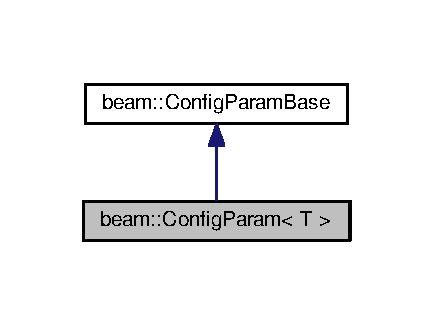
\includegraphics[width=208pt]{classbeam_1_1_config_param__inherit__graph}
\end{center}
\end{figure}


Collaboration diagram for beam\+:\+:Config\+Param$<$ T $>$\+:\nopagebreak
\begin{figure}[H]
\begin{center}
\leavevmode
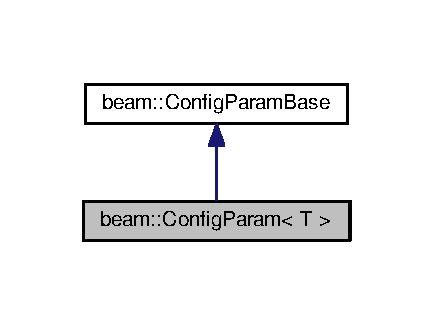
\includegraphics[width=208pt]{classbeam_1_1_config_param__coll__graph}
\end{center}
\end{figure}
\subsection*{Public Member Functions}
\begin{DoxyCompactItemize}
\item 
\hyperlink{classbeam_1_1_config_param_aaa594f071a53dfda2294c758d46a7330}{Config\+Param} (std\+::string \hyperlink{structbeam_1_1_config_param_base_afbf349bc86d925088544d04a24c484b0}{key}, T $\ast$destination, bool \hyperlink{structbeam_1_1_config_param_base_a4c73616a18786e1885265a02dbf8b9a5}{optional}=false)
\item 
void \hyperlink{classbeam_1_1_config_param_a805133e6dae35596e1383a6d223f4dc3}{load} (const Y\+A\+M\+L\+::\+Node \&node) const override
\end{DoxyCompactItemize}
\subsection*{Protected Attributes}
\begin{DoxyCompactItemize}
\item 
T $\ast$ \hyperlink{classbeam_1_1_config_param_a1f5a1becff7e710e61bbc0dac8289ce8}{data} = nullptr
\begin{DoxyCompactList}\small\item\em where we will store the parsed value \end{DoxyCompactList}\end{DoxyCompactItemize}
\subsection*{Additional Inherited Members}


\subsection{Detailed Description}
\subsubsection*{template$<$typename T$>$\\*
class beam\+::\+Config\+Param$<$ T $>$}

Represents a parameter to be parsed in the yaml file 

Definition at line 56 of file config.\+hpp.



\subsection{Constructor \& Destructor Documentation}
\index{beam\+::\+Config\+Param@{beam\+::\+Config\+Param}!Config\+Param@{Config\+Param}}
\index{Config\+Param@{Config\+Param}!beam\+::\+Config\+Param@{beam\+::\+Config\+Param}}
\subsubsection[{\texorpdfstring{Config\+Param(std\+::string key, T $\ast$destination, bool optional=false)}{ConfigParam(std::string key, T *destination, bool optional=false)}}]{\setlength{\rightskip}{0pt plus 5cm}template$<$typename T $>$ {\bf beam\+::\+Config\+Param}$<$ T $>$\+::{\bf Config\+Param} (
\begin{DoxyParamCaption}
\item[{std\+::string}]{key, }
\item[{T $\ast$}]{destination, }
\item[{bool}]{optional = {\ttfamily false}}
\end{DoxyParamCaption}
)\hspace{0.3cm}{\ttfamily [inline]}}\hypertarget{classbeam_1_1_config_param_aaa594f071a53dfda2294c758d46a7330}{}\label{classbeam_1_1_config_param_aaa594f071a53dfda2294c758d46a7330}


Definition at line 58 of file config.\+hpp.



\subsection{Member Function Documentation}
\index{beam\+::\+Config\+Param@{beam\+::\+Config\+Param}!load@{load}}
\index{load@{load}!beam\+::\+Config\+Param@{beam\+::\+Config\+Param}}
\subsubsection[{\texorpdfstring{load(const Y\+A\+M\+L\+::\+Node \&node) const override}{load(const YAML::Node &node) const override}}]{\setlength{\rightskip}{0pt plus 5cm}template$<$typename T $>$ void {\bf beam\+::\+Config\+Param}$<$ T $>$\+::load (
\begin{DoxyParamCaption}
\item[{const Y\+A\+M\+L\+::\+Node \&}]{node}
\end{DoxyParamCaption}
) const\hspace{0.3cm}{\ttfamily [inline]}, {\ttfamily [override]}, {\ttfamily [virtual]}}\hypertarget{classbeam_1_1_config_param_a805133e6dae35596e1383a6d223f4dc3}{}\label{classbeam_1_1_config_param_a805133e6dae35596e1383a6d223f4dc3}
Parse the given node as T, and write the value into {\ttfamily destination}. \begin{DoxyNote}{Note}
no lookup by key is performed; the node must already be correct 
\end{DoxyNote}

\begin{DoxyExceptions}{Exceptions}
{\em Y\+A\+M\+L\+::\+Bad\+Conversion} & if node is not convertible to destination \\
\hline
\end{DoxyExceptions}


Implements \hyperlink{structbeam_1_1_config_param_base_af4d235d401db493e99acf96065d36c73}{beam\+::\+Config\+Param\+Base}.



Definition at line 65 of file config.\+hpp.



\subsection{Member Data Documentation}
\index{beam\+::\+Config\+Param@{beam\+::\+Config\+Param}!data@{data}}
\index{data@{data}!beam\+::\+Config\+Param@{beam\+::\+Config\+Param}}
\subsubsection[{\texorpdfstring{data}{data}}]{\setlength{\rightskip}{0pt plus 5cm}template$<$typename T $>$ T$\ast$ {\bf beam\+::\+Config\+Param}$<$ T $>$\+::data = nullptr\hspace{0.3cm}{\ttfamily [protected]}}\hypertarget{classbeam_1_1_config_param_a1f5a1becff7e710e61bbc0dac8289ce8}{}\label{classbeam_1_1_config_param_a1f5a1becff7e710e61bbc0dac8289ce8}


where we will store the parsed value 



Definition at line 70 of file config.\+hpp.



The documentation for this class was generated from the following file\+:\begin{DoxyCompactItemize}
\item 
beam\+\_\+utils/include/beam/utils/\hyperlink{config_8hpp}{config.\+hpp}\end{DoxyCompactItemize}

\hypertarget{structbeam_1_1_config_param_base}{}\section{beam\+:\+:Config\+Param\+Base Struct Reference}
\label{structbeam_1_1_config_param_base}\index{beam\+::\+Config\+Param\+Base@{beam\+::\+Config\+Param\+Base}}


{\ttfamily \#include $<$config.\+hpp$>$}



Inheritance diagram for beam\+:\+:Config\+Param\+Base\+:\nopagebreak
\begin{figure}[H]
\begin{center}
\leavevmode
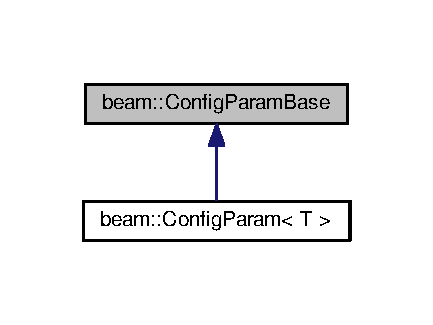
\includegraphics[width=208pt]{structbeam_1_1_config_param_base__inherit__graph}
\end{center}
\end{figure}
\subsection*{Public Member Functions}
\begin{DoxyCompactItemize}
\item 
\hyperlink{structbeam_1_1_config_param_base_a9dbdaedbcc8610bd09390d570490a243}{Config\+Param\+Base} (std\+::string \hyperlink{structbeam_1_1_config_param_base_afbf349bc86d925088544d04a24c484b0}{key}, bool \hyperlink{structbeam_1_1_config_param_base_a4c73616a18786e1885265a02dbf8b9a5}{optional})
\item 
virtual void \hyperlink{structbeam_1_1_config_param_base_af4d235d401db493e99acf96065d36c73}{load} (const Y\+A\+M\+L\+::\+Node \&node) const =0
\end{DoxyCompactItemize}
\subsection*{Public Attributes}
\begin{DoxyCompactItemize}
\item 
std\+::string \hyperlink{structbeam_1_1_config_param_base_afbf349bc86d925088544d04a24c484b0}{key}
\begin{DoxyCompactList}\small\item\em yaml key to parse from \end{DoxyCompactList}\item 
bool \hyperlink{structbeam_1_1_config_param_base_a4c73616a18786e1885265a02dbf8b9a5}{optional}
\begin{DoxyCompactList}\small\item\em if true, it is not an error if the key is not found \end{DoxyCompactList}\end{DoxyCompactItemize}
\subsection*{Protected Member Functions}
\begin{DoxyCompactItemize}
\item 
\hyperlink{structbeam_1_1_config_param_base_a876d21f911d6920231329e96a311298a}{$\sim$\+Config\+Param\+Base} ()=default
\end{DoxyCompactItemize}


\subsection{Detailed Description}
Base class representing a parameter to be parsed in the yaml file 

Definition at line 37 of file config.\+hpp.



\subsection{Constructor \& Destructor Documentation}
\index{beam\+::\+Config\+Param\+Base@{beam\+::\+Config\+Param\+Base}!Config\+Param\+Base@{Config\+Param\+Base}}
\index{Config\+Param\+Base@{Config\+Param\+Base}!beam\+::\+Config\+Param\+Base@{beam\+::\+Config\+Param\+Base}}
\subsubsection[{\texorpdfstring{Config\+Param\+Base(std\+::string key, bool optional)}{ConfigParamBase(std::string key, bool optional)}}]{\setlength{\rightskip}{0pt plus 5cm}beam\+::\+Config\+Param\+Base\+::\+Config\+Param\+Base (
\begin{DoxyParamCaption}
\item[{std\+::string}]{key, }
\item[{bool}]{optional}
\end{DoxyParamCaption}
)\hspace{0.3cm}{\ttfamily [inline]}}\hypertarget{structbeam_1_1_config_param_base_a9dbdaedbcc8610bd09390d570490a243}{}\label{structbeam_1_1_config_param_base_a9dbdaedbcc8610bd09390d570490a243}


Definition at line 38 of file config.\+hpp.

\index{beam\+::\+Config\+Param\+Base@{beam\+::\+Config\+Param\+Base}!````~Config\+Param\+Base@{$\sim$\+Config\+Param\+Base}}
\index{````~Config\+Param\+Base@{$\sim$\+Config\+Param\+Base}!beam\+::\+Config\+Param\+Base@{beam\+::\+Config\+Param\+Base}}
\subsubsection[{\texorpdfstring{$\sim$\+Config\+Param\+Base()=default}{~ConfigParamBase()=default}}]{\setlength{\rightskip}{0pt plus 5cm}beam\+::\+Config\+Param\+Base\+::$\sim$\+Config\+Param\+Base (
\begin{DoxyParamCaption}
{}
\end{DoxyParamCaption}
)\hspace{0.3cm}{\ttfamily [protected]}, {\ttfamily [default]}}\hypertarget{structbeam_1_1_config_param_base_a876d21f911d6920231329e96a311298a}{}\label{structbeam_1_1_config_param_base_a876d21f911d6920231329e96a311298a}


\subsection{Member Function Documentation}
\index{beam\+::\+Config\+Param\+Base@{beam\+::\+Config\+Param\+Base}!load@{load}}
\index{load@{load}!beam\+::\+Config\+Param\+Base@{beam\+::\+Config\+Param\+Base}}
\subsubsection[{\texorpdfstring{load(const Y\+A\+M\+L\+::\+Node \&node) const =0}{load(const YAML::Node &node) const =0}}]{\setlength{\rightskip}{0pt plus 5cm}virtual void beam\+::\+Config\+Param\+Base\+::load (
\begin{DoxyParamCaption}
\item[{const Y\+A\+M\+L\+::\+Node \&}]{node}
\end{DoxyParamCaption}
) const\hspace{0.3cm}{\ttfamily [pure virtual]}}\hypertarget{structbeam_1_1_config_param_base_af4d235d401db493e99acf96065d36c73}{}\label{structbeam_1_1_config_param_base_af4d235d401db493e99acf96065d36c73}
Parse the given node as T, and write the value into {\ttfamily destination}. \begin{DoxyNote}{Note}
no lookup by key is performed; the node must already be correct 
\end{DoxyNote}

\begin{DoxyExceptions}{Exceptions}
{\em Y\+A\+M\+L\+::\+Bad\+Conversion} & if node is not convertible to destination \\
\hline
\end{DoxyExceptions}


Implemented in \hyperlink{classbeam_1_1_config_param_a805133e6dae35596e1383a6d223f4dc3}{beam\+::\+Config\+Param$<$ T $>$}.



\subsection{Member Data Documentation}
\index{beam\+::\+Config\+Param\+Base@{beam\+::\+Config\+Param\+Base}!key@{key}}
\index{key@{key}!beam\+::\+Config\+Param\+Base@{beam\+::\+Config\+Param\+Base}}
\subsubsection[{\texorpdfstring{key}{key}}]{\setlength{\rightskip}{0pt plus 5cm}std\+::string beam\+::\+Config\+Param\+Base\+::key}\hypertarget{structbeam_1_1_config_param_base_afbf349bc86d925088544d04a24c484b0}{}\label{structbeam_1_1_config_param_base_afbf349bc86d925088544d04a24c484b0}


yaml key to parse from 



Definition at line 47 of file config.\+hpp.

\index{beam\+::\+Config\+Param\+Base@{beam\+::\+Config\+Param\+Base}!optional@{optional}}
\index{optional@{optional}!beam\+::\+Config\+Param\+Base@{beam\+::\+Config\+Param\+Base}}
\subsubsection[{\texorpdfstring{optional}{optional}}]{\setlength{\rightskip}{0pt plus 5cm}bool beam\+::\+Config\+Param\+Base\+::optional}\hypertarget{structbeam_1_1_config_param_base_a4c73616a18786e1885265a02dbf8b9a5}{}\label{structbeam_1_1_config_param_base_a4c73616a18786e1885265a02dbf8b9a5}


if true, it is not an error if the key is not found 



Definition at line 48 of file config.\+hpp.



The documentation for this struct was generated from the following file\+:\begin{DoxyCompactItemize}
\item 
beam\+\_\+utils/include/beam/utils/\hyperlink{config_8hpp}{config.\+hpp}\end{DoxyCompactItemize}

\hypertarget{classbeam_1_1_config_parser}{}\section{beam\+:\+:Config\+Parser Class Reference}
\label{classbeam_1_1_config_parser}\index{beam\+::\+Config\+Parser@{beam\+::\+Config\+Parser}}


{\ttfamily \#include $<$config.\+hpp$>$}

\subsection*{Public Member Functions}
\begin{DoxyCompactItemize}
\item 
\hyperlink{classbeam_1_1_config_parser_a1f2a583c9eb00c93da60d14711b4389a}{Config\+Parser} (void)
\item 
{\footnotesize template$<$typename T $>$ }\\void \hyperlink{classbeam_1_1_config_parser_a06f647e3b6a20452877dda482854fa8c}{add\+Param} (std\+::string key, T $\ast$out, bool optional=false)
\item 
\hyperlink{group__utils_ga6b948c6f49abd3a3de95390efacfba63}{Config\+Status} \hyperlink{classbeam_1_1_config_parser_a347d9487325f54f158b2c6d748c38448}{get\+Yaml\+Node} (const std\+::string \&key, Y\+A\+M\+L\+::\+Node \&node)
\item 
\hyperlink{group__utils_ga6b948c6f49abd3a3de95390efacfba63}{Config\+Status} \hyperlink{classbeam_1_1_config_parser_a908bfee0c4dda2fda2a6deae9edd98df}{check\+Key} (const std\+::string \&key, bool optional)
\item 
\hyperlink{group__utils_ga6b948c6f49abd3a3de95390efacfba63}{Config\+Status} \hyperlink{classbeam_1_1_config_parser_a990c530e4f94f88a81d46c8fd38bbd92}{load\+Param} (const \hyperlink{structbeam_1_1_config_param_base}{Config\+Param\+Base} \&param)
\item 
\hyperlink{group__utils_ga6b948c6f49abd3a3de95390efacfba63}{Config\+Status} \hyperlink{classbeam_1_1_config_parser_a28dd7f968674139ed0bbc4fcdb01f514}{load} (const std\+::string \&config\+\_\+file)
\end{DoxyCompactItemize}
\subsection*{Public Attributes}
\begin{DoxyCompactItemize}
\item 
bool \hyperlink{classbeam_1_1_config_parser_a4d9b8c9944779dfccae586ac3a337987}{config\+\_\+loaded}
\item 
Y\+A\+M\+L\+::\+Node \hyperlink{classbeam_1_1_config_parser_af7194358406b989236ad11515a19d963}{root}
\item 
std\+::vector$<$ std\+::shared\+\_\+ptr$<$ \hyperlink{structbeam_1_1_config_param_base}{Config\+Param\+Base} $>$ $>$ \hyperlink{classbeam_1_1_config_parser_adb1a9f52c1ee4bf974088519237dcefc}{params}
\end{DoxyCompactItemize}


\subsection{Detailed Description}
Parses yaml files for parameters of different types.

Currently {\ttfamily \hyperlink{classbeam_1_1_config_parser}{Config\+Parser}} supports parsing the following data types\+:
\begin{DoxyItemize}
\item {\bfseries Primitives}\+: {\ttfamily bool}, {\ttfamily int}, {\ttfamily float}, {\ttfamily double}, {\ttfamily std\+::string}
\item {\bfseries Arrays}\+: {\ttfamily std\+::vector$<$bool$>$}, {\ttfamily std\+::vector$<$int$>$}, {\ttfamily std\+::vector$<$float$>$}, {\ttfamily std\+::vector$<$double$>$}, {\ttfamily std\+::vector$<$std\+::string$>$}
\item {\bfseries Vectors}\+: {\ttfamily Eigen\+::\+Vector2d}, {\ttfamily Eigen\+::\+Vector3d}, {\ttfamily Eigen\+::\+Vector4d}, {\ttfamily Eigen\+::\+Vector\+Xd}
\item {\bfseries Matrices}\+: {\ttfamily Eigen\+::\+Matrix2d}, {\ttfamily Eigen\+::\+Matrix3d}, {\ttfamily Eigen\+::\+Matrix4d}, {\ttfamily Eigen\+::\+Matrix\+Xd}
\end{DoxyItemize}

\begin{DoxyNote}{Note}
For a {\bfseries matrix} we require the yaml to have three nested keys in order for {\ttfamily \hyperlink{classbeam_1_1_config_parser}{Config\+Parser}} to operate properly. They are {\ttfamily rows}, {\ttfamily cols} and {\ttfamily data}. For example\+: 
\begin{DoxyCode}
1 some\_matrix:
2   rows: 3
3   cols: 3
4   data: [1.1, 2.2, 3.3,
5          4.4, 5.5, 6.6,
6          7.7, 8.8, 9.9]
\end{DoxyCode}

\end{DoxyNote}
For example, consider this yaml file\+: 
\begin{DoxyCodeInclude}
\end{DoxyCodeInclude}


The code that parses the above is\+: 
\begin{DoxyCodeInclude}
\end{DoxyCodeInclude}


\begin{DoxyRefDesc}{Todo}
\item[\hyperlink{todo__todo000001}{Todo}]integrate unit tests into examples (see \href{http://stackoverflow.com/a/16034375/431033}{\tt http\+://stackoverflow.\+com/a/16034375/431033}) \end{DoxyRefDesc}


Definition at line 105 of file config.\+hpp.



\subsection{Constructor \& Destructor Documentation}
\index{beam\+::\+Config\+Parser@{beam\+::\+Config\+Parser}!Config\+Parser@{Config\+Parser}}
\index{Config\+Parser@{Config\+Parser}!beam\+::\+Config\+Parser@{beam\+::\+Config\+Parser}}
\subsubsection[{\texorpdfstring{Config\+Parser(void)}{ConfigParser(void)}}]{\setlength{\rightskip}{0pt plus 5cm}beam\+::\+Config\+Parser\+::\+Config\+Parser (
\begin{DoxyParamCaption}
\item[{void}]{}
\end{DoxyParamCaption}
)}\hypertarget{classbeam_1_1_config_parser_a1f2a583c9eb00c93da60d14711b4389a}{}\label{classbeam_1_1_config_parser_a1f2a583c9eb00c93da60d14711b4389a}
Default constructor. By default it sets\+:


\begin{DoxyItemize}
\item {\ttfamily config\+\_\+loaded} to {\ttfamily false}
\end{DoxyItemize}

This variable is set to {\ttfamily true} once the yaml file is loaded. 

Definition at line 6 of file config.\+cpp.



\subsection{Member Function Documentation}
\index{beam\+::\+Config\+Parser@{beam\+::\+Config\+Parser}!add\+Param@{add\+Param}}
\index{add\+Param@{add\+Param}!beam\+::\+Config\+Parser@{beam\+::\+Config\+Parser}}
\subsubsection[{\texorpdfstring{add\+Param(std\+::string key, T $\ast$out, bool optional=false)}{addParam(std::string key, T *out, bool optional=false)}}]{\setlength{\rightskip}{0pt plus 5cm}template$<$typename T $>$ void beam\+::\+Config\+Parser\+::add\+Param (
\begin{DoxyParamCaption}
\item[{std\+::string}]{key, }
\item[{T $\ast$}]{out, }
\item[{bool}]{optional = {\ttfamily false}}
\end{DoxyParamCaption}
)\hspace{0.3cm}{\ttfamily [inline]}}\hypertarget{classbeam_1_1_config_parser_a06f647e3b6a20452877dda482854fa8c}{}\label{classbeam_1_1_config_parser_a06f647e3b6a20452877dda482854fa8c}
Use the variations of {\ttfamily add\+Param} to add parameters you would like to parse from the yaml file, where {\ttfamily key} is the yaml key, {\ttfamily out} is dependent on the type of parameter you want to parse to and an {\ttfamily optional} parameter to define whether {\ttfamily \hyperlink{classbeam_1_1_config_parser}{Config\+Parser}} should fail if the parameter is not found. 

Definition at line 127 of file config.\+hpp.

\index{beam\+::\+Config\+Parser@{beam\+::\+Config\+Parser}!check\+Key@{check\+Key}}
\index{check\+Key@{check\+Key}!beam\+::\+Config\+Parser@{beam\+::\+Config\+Parser}}
\subsubsection[{\texorpdfstring{check\+Key(const std\+::string \&key, bool optional)}{checkKey(const std::string &key, bool optional)}}]{\setlength{\rightskip}{0pt plus 5cm}{\bf Config\+Status} beam\+::\+Config\+Parser\+::check\+Key (
\begin{DoxyParamCaption}
\item[{const std\+::string \&}]{key, }
\item[{bool}]{optional}
\end{DoxyParamCaption}
)}\hypertarget{classbeam_1_1_config_parser_a908bfee0c4dda2fda2a6deae9edd98df}{}\label{classbeam_1_1_config_parser_a908bfee0c4dda2fda2a6deae9edd98df}
Check whether a key is present in the yaml file 

Definition at line 38 of file config.\+cpp.

\index{beam\+::\+Config\+Parser@{beam\+::\+Config\+Parser}!get\+Yaml\+Node@{get\+Yaml\+Node}}
\index{get\+Yaml\+Node@{get\+Yaml\+Node}!beam\+::\+Config\+Parser@{beam\+::\+Config\+Parser}}
\subsubsection[{\texorpdfstring{get\+Yaml\+Node(const std\+::string \&key, Y\+A\+M\+L\+::\+Node \&node)}{getYamlNode(const std::string &key, YAML::Node &node)}}]{\setlength{\rightskip}{0pt plus 5cm}{\bf Config\+Status} beam\+::\+Config\+Parser\+::get\+Yaml\+Node (
\begin{DoxyParamCaption}
\item[{const std\+::string \&}]{key, }
\item[{Y\+A\+M\+L\+::\+Node \&}]{node}
\end{DoxyParamCaption}
)}\hypertarget{classbeam_1_1_config_parser_a347d9487325f54f158b2c6d748c38448}{}\label{classbeam_1_1_config_parser_a347d9487325f54f158b2c6d748c38448}
Get yaml node given yaml {\ttfamily key}. The result is assigned to {\ttfamily node} if {\ttfamily key} matches anything in the config file, else {\ttfamily node} is set to {\ttfamily N\+U\+LL}. 

Definition at line 10 of file config.\+cpp.

\index{beam\+::\+Config\+Parser@{beam\+::\+Config\+Parser}!load@{load}}
\index{load@{load}!beam\+::\+Config\+Parser@{beam\+::\+Config\+Parser}}
\subsubsection[{\texorpdfstring{load(const std\+::string \&config\+\_\+file)}{load(const std::string &config_file)}}]{\setlength{\rightskip}{0pt plus 5cm}{\bf Config\+Status} beam\+::\+Config\+Parser\+::load (
\begin{DoxyParamCaption}
\item[{const std\+::string \&}]{config\+\_\+file}
\end{DoxyParamCaption}
)}\hypertarget{classbeam_1_1_config_parser_a28dd7f968674139ed0bbc4fcdb01f514}{}\label{classbeam_1_1_config_parser_a28dd7f968674139ed0bbc4fcdb01f514}
Load yaml file at {\ttfamily config\+\_\+file}. 

Definition at line 80 of file config.\+cpp.

\index{beam\+::\+Config\+Parser@{beam\+::\+Config\+Parser}!load\+Param@{load\+Param}}
\index{load\+Param@{load\+Param}!beam\+::\+Config\+Parser@{beam\+::\+Config\+Parser}}
\subsubsection[{\texorpdfstring{load\+Param(const Config\+Param\+Base \&param)}{loadParam(const ConfigParamBase &param)}}]{\setlength{\rightskip}{0pt plus 5cm}{\bf Config\+Status} beam\+::\+Config\+Parser\+::load\+Param (
\begin{DoxyParamCaption}
\item[{const {\bf Config\+Param\+Base} \&}]{param}
\end{DoxyParamCaption}
)}\hypertarget{classbeam_1_1_config_parser_a990c530e4f94f88a81d46c8fd38bbd92}{}\label{classbeam_1_1_config_parser_a990c530e4f94f88a81d46c8fd38bbd92}
Load yaml param primitive, array, vector or matrix. 

Definition at line 58 of file config.\+cpp.



\subsection{Member Data Documentation}
\index{beam\+::\+Config\+Parser@{beam\+::\+Config\+Parser}!config\+\_\+loaded@{config\+\_\+loaded}}
\index{config\+\_\+loaded@{config\+\_\+loaded}!beam\+::\+Config\+Parser@{beam\+::\+Config\+Parser}}
\subsubsection[{\texorpdfstring{config\+\_\+loaded}{config_loaded}}]{\setlength{\rightskip}{0pt plus 5cm}bool beam\+::\+Config\+Parser\+::config\+\_\+loaded}\hypertarget{classbeam_1_1_config_parser_a4d9b8c9944779dfccae586ac3a337987}{}\label{classbeam_1_1_config_parser_a4d9b8c9944779dfccae586ac3a337987}


Definition at line 107 of file config.\+hpp.

\index{beam\+::\+Config\+Parser@{beam\+::\+Config\+Parser}!params@{params}}
\index{params@{params}!beam\+::\+Config\+Parser@{beam\+::\+Config\+Parser}}
\subsubsection[{\texorpdfstring{params}{params}}]{\setlength{\rightskip}{0pt plus 5cm}std\+::vector$<$std\+::shared\+\_\+ptr$<${\bf Config\+Param\+Base}$>$ $>$ beam\+::\+Config\+Parser\+::params}\hypertarget{classbeam_1_1_config_parser_adb1a9f52c1ee4bf974088519237dcefc}{}\label{classbeam_1_1_config_parser_adb1a9f52c1ee4bf974088519237dcefc}


Definition at line 110 of file config.\+hpp.

\index{beam\+::\+Config\+Parser@{beam\+::\+Config\+Parser}!root@{root}}
\index{root@{root}!beam\+::\+Config\+Parser@{beam\+::\+Config\+Parser}}
\subsubsection[{\texorpdfstring{root}{root}}]{\setlength{\rightskip}{0pt plus 5cm}Y\+A\+M\+L\+::\+Node beam\+::\+Config\+Parser\+::root}\hypertarget{classbeam_1_1_config_parser_af7194358406b989236ad11515a19d963}{}\label{classbeam_1_1_config_parser_af7194358406b989236ad11515a19d963}


Definition at line 109 of file config.\+hpp.



The documentation for this class was generated from the following files\+:\begin{DoxyCompactItemize}
\item 
beam\+\_\+utils/include/beam/utils/\hyperlink{config_8hpp}{config.\+hpp}\item 
beam\+\_\+utils/src/\hyperlink{config_8cpp}{config.\+cpp}\end{DoxyCompactItemize}

\hypertarget{struct_y_a_m_l_1_1convert_3_01_eigen_1_1_matrix_3_01_scalar_00_01_rows_00_011_01_4_01_4}{}\section{Y\+A\+ML\+:\+:convert$<$ Eigen\+:\+:Matrix$<$ Scalar, Rows, 1 $>$ $>$ Struct Template Reference}
\label{struct_y_a_m_l_1_1convert_3_01_eigen_1_1_matrix_3_01_scalar_00_01_rows_00_011_01_4_01_4}\index{Y\+A\+M\+L\+::convert$<$ Eigen\+::\+Matrix$<$ Scalar, Rows, 1 $>$ $>$@{Y\+A\+M\+L\+::convert$<$ Eigen\+::\+Matrix$<$ Scalar, Rows, 1 $>$ $>$}}


{\ttfamily \#include $<$config.\+hpp$>$}

\subsection*{Static Public Member Functions}
\begin{DoxyCompactItemize}
\item 
static bool \hyperlink{struct_y_a_m_l_1_1convert_3_01_eigen_1_1_matrix_3_01_scalar_00_01_rows_00_011_01_4_01_4_ab055b0f7ee0b46864b1df4692e3a0050}{decode} (const Node \&node, Eigen\+::\+Matrix$<$ Scalar, Rows, 1 $>$ \&out)
\end{DoxyCompactItemize}


\subsection{Detailed Description}
\subsubsection*{template$<$typename Scalar, int Rows$>$\\*
struct Y\+A\+M\+L\+::convert$<$ Eigen\+::\+Matrix$<$ Scalar, Rows, 1 $>$ $>$}

Custom conversion functions for \hyperlink{namespace_y_a_m_l}{Y\+A\+ML} -\/$>$ Eigen vector

For example\+: 
\begin{DoxyCode}
1 some\_vector: [1.1, 2.2, 3.3]
\end{DoxyCode}


Conversions for the following types are compiled as part of beam\+\_\+utils\+:
\begin{DoxyItemize}
\item Eigen\+::\+Vector2d
\item Eigen\+::\+Vector3d
\item Eigen\+::\+Vector4d
\item Eigen\+::\+Vector\+Xd 
\end{DoxyItemize}

Definition at line 197 of file config.\+hpp.



\subsection{Member Function Documentation}
\index{Y\+A\+M\+L\+::convert$<$ Eigen\+::\+Matrix$<$ Scalar, Rows, 1 $>$ $>$@{Y\+A\+M\+L\+::convert$<$ Eigen\+::\+Matrix$<$ Scalar, Rows, 1 $>$ $>$}!decode@{decode}}
\index{decode@{decode}!Y\+A\+M\+L\+::convert$<$ Eigen\+::\+Matrix$<$ Scalar, Rows, 1 $>$ $>$@{Y\+A\+M\+L\+::convert$<$ Eigen\+::\+Matrix$<$ Scalar, Rows, 1 $>$ $>$}}
\subsubsection[{\texorpdfstring{decode(const Node \&node, Eigen\+::\+Matrix$<$ Scalar, Rows, 1 $>$ \&out)}{decode(const Node &node, Eigen::Matrix< Scalar, Rows, 1 > &out)}}]{\setlength{\rightskip}{0pt plus 5cm}template$<$typename Scalar , int Rows$>$ bool Y\+A\+M\+L\+::convert$<$ Eigen\+::\+Matrix$<$ Scalar, Rows, 1 $>$ $>$\+::decode (
\begin{DoxyParamCaption}
\item[{const Node \&}]{node, }
\item[{Eigen\+::\+Matrix$<$ Scalar, Rows, 1 $>$ \&}]{out}
\end{DoxyParamCaption}
)\hspace{0.3cm}{\ttfamily [static]}}\hypertarget{struct_y_a_m_l_1_1convert_3_01_eigen_1_1_matrix_3_01_scalar_00_01_rows_00_011_01_4_01_4_ab055b0f7ee0b46864b1df4692e3a0050}{}\label{struct_y_a_m_l_1_1convert_3_01_eigen_1_1_matrix_3_01_scalar_00_01_rows_00_011_01_4_01_4_ab055b0f7ee0b46864b1df4692e3a0050}
Convert \hyperlink{namespace_y_a_m_l}{Y\+A\+ML} node to Eigen Matrix \begin{DoxyReturn}{Returns}
true if conversion successful 
\end{DoxyReturn}


Definition at line 140 of file config.\+cpp.



The documentation for this struct was generated from the following files\+:\begin{DoxyCompactItemize}
\item 
beam\+\_\+utils/include/beam/utils/\hyperlink{config_8hpp}{config.\+hpp}\item 
beam\+\_\+utils/src/\hyperlink{config_8cpp}{config.\+cpp}\end{DoxyCompactItemize}

\hypertarget{struct_y_a_m_l_1_1convert_3_01_eigen_1_1_matrix_3_01_scalar_00_01_rows_00_01_cols_01_4_01_4}{}\section{Y\+A\+ML\+:\+:convert$<$ Eigen\+:\+:Matrix$<$ Scalar, Rows, Cols $>$ $>$ Struct Template Reference}
\label{struct_y_a_m_l_1_1convert_3_01_eigen_1_1_matrix_3_01_scalar_00_01_rows_00_01_cols_01_4_01_4}\index{Y\+A\+M\+L\+::convert$<$ Eigen\+::\+Matrix$<$ Scalar, Rows, Cols $>$ $>$@{Y\+A\+M\+L\+::convert$<$ Eigen\+::\+Matrix$<$ Scalar, Rows, Cols $>$ $>$}}


{\ttfamily \#include $<$config.\+hpp$>$}

\subsection*{Static Public Member Functions}
\begin{DoxyCompactItemize}
\item 
static bool \hyperlink{struct_y_a_m_l_1_1convert_3_01_eigen_1_1_matrix_3_01_scalar_00_01_rows_00_01_cols_01_4_01_4_aaceb24ec400b99197353373ef2c29a11}{decode} (const Node \&node, Eigen\+::\+Matrix$<$ Scalar, Rows, Cols $>$ \&out)
\end{DoxyCompactItemize}


\subsection{Detailed Description}
\subsubsection*{template$<$typename Scalar, int Rows, int Cols$>$\\*
struct Y\+A\+M\+L\+::convert$<$ Eigen\+::\+Matrix$<$ Scalar, Rows, Cols $>$ $>$}

Custom conversion functions for \hyperlink{namespace_y_a_m_l}{Y\+A\+ML} -\/$>$ Eigen matrix

\begin{DoxyNote}{Note}
We require the yaml node to have three nested keys in order to parse a matrix. They are {\ttfamily rows}, {\ttfamily cols} and {\ttfamily data}.
\end{DoxyNote}
For example\+: 
\begin{DoxyCode}
1 some\_matrix:
2   rows: 3
3   cols: 3
4   data: [1.1, 2.2, 3.3,
5          4.4, 5.5, 6.6,
6          7.7, 8.8, 9.9]
\end{DoxyCode}


Conversions for the following types are included in of beam\+\_\+utils\+:
\begin{DoxyItemize}
\item Eigen\+::\+Matrix2d
\item Eigen\+::\+Matrix3d
\item Eigen\+::\+Matrix4d
\item Eigen\+::\+Matrix\+Xd 
\end{DoxyItemize}

Definition at line 174 of file config.\+hpp.



\subsection{Member Function Documentation}
\index{Y\+A\+M\+L\+::convert$<$ Eigen\+::\+Matrix$<$ Scalar, Rows, Cols $>$ $>$@{Y\+A\+M\+L\+::convert$<$ Eigen\+::\+Matrix$<$ Scalar, Rows, Cols $>$ $>$}!decode@{decode}}
\index{decode@{decode}!Y\+A\+M\+L\+::convert$<$ Eigen\+::\+Matrix$<$ Scalar, Rows, Cols $>$ $>$@{Y\+A\+M\+L\+::convert$<$ Eigen\+::\+Matrix$<$ Scalar, Rows, Cols $>$ $>$}}
\subsubsection[{\texorpdfstring{decode(const Node \&node, Eigen\+::\+Matrix$<$ Scalar, Rows, Cols $>$ \&out)}{decode(const Node &node, Eigen::Matrix< Scalar, Rows, Cols > &out)}}]{\setlength{\rightskip}{0pt plus 5cm}template$<$typename Scalar , int Rows, int Cols$>$ bool Y\+A\+M\+L\+::convert$<$ Eigen\+::\+Matrix$<$ Scalar, Rows, Cols $>$ $>$\+::decode (
\begin{DoxyParamCaption}
\item[{const Node \&}]{node, }
\item[{Eigen\+::\+Matrix$<$ Scalar, Rows, Cols $>$ \&}]{out}
\end{DoxyParamCaption}
)\hspace{0.3cm}{\ttfamily [static]}}\hypertarget{struct_y_a_m_l_1_1convert_3_01_eigen_1_1_matrix_3_01_scalar_00_01_rows_00_01_cols_01_4_01_4_aaceb24ec400b99197353373ef2c29a11}{}\label{struct_y_a_m_l_1_1convert_3_01_eigen_1_1_matrix_3_01_scalar_00_01_rows_00_01_cols_01_4_01_4_aaceb24ec400b99197353373ef2c29a11}
Convert \hyperlink{namespace_y_a_m_l}{Y\+A\+ML} node to Eigen Matrix


\begin{DoxyExceptions}{Exceptions}
{\em Y\+A\+M\+L\+::\+Invalid\+Node} & if nested keys not found \\
\hline
\end{DoxyExceptions}
\begin{DoxyReturn}{Returns}
true if conversion successful 
\end{DoxyReturn}


Definition at line 110 of file config.\+cpp.



The documentation for this struct was generated from the following files\+:\begin{DoxyCompactItemize}
\item 
beam\+\_\+utils/include/beam/utils/\hyperlink{config_8hpp}{config.\+hpp}\item 
beam\+\_\+utils/src/\hyperlink{config_8cpp}{config.\+cpp}\end{DoxyCompactItemize}

\hypertarget{classbeam__defects_1_1_crack}{}\section{beam\+\_\+defects\+:\+:Crack Class Reference}
\label{classbeam__defects_1_1_crack}\index{beam\+\_\+defects\+::\+Crack@{beam\+\_\+defects\+::\+Crack}}


Derived class for crack defects.  




{\ttfamily \#include $<$Crack.\+h$>$}



Inheritance diagram for beam\+\_\+defects\+:\+:Crack\+:\nopagebreak
\begin{figure}[H]
\begin{center}
\leavevmode
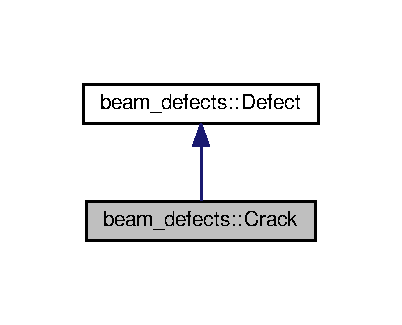
\includegraphics[width=193pt]{classbeam__defects_1_1_crack__inherit__graph}
\end{center}
\end{figure}


Collaboration diagram for beam\+\_\+defects\+:\+:Crack\+:\nopagebreak
\begin{figure}[H]
\begin{center}
\leavevmode
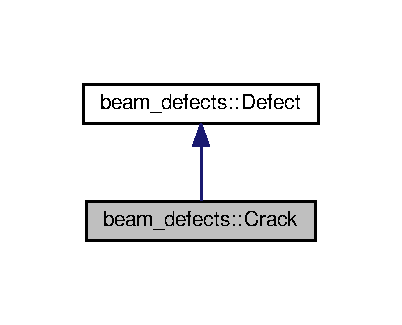
\includegraphics[width=193pt]{classbeam__defects_1_1_crack__coll__graph}
\end{center}
\end{figure}
\subsection*{Public Member Functions}
\begin{DoxyCompactItemize}
\item 
\hyperlink{classbeam__defects_1_1_crack_ada9aa870e95e7799bc609891cb586d13}{Crack} ()=default
\begin{DoxyCompactList}\small\item\em Default constructor. \end{DoxyCompactList}\item 
\hyperlink{classbeam__defects_1_1_crack_a29c3ebe842c944977cbe981b3d33c6de}{Crack} (pcl\+::\+Point\+Cloud$<$ pcl\+::\+Point\+X\+YZ $>$\+::\hyperlink{classbeam__defects_1_1_defect_a0a7708c6cd92ac482d45ef606d598325}{Ptr} pc)
\begin{DoxyCompactList}\small\item\em Construct with a point cloud. \end{DoxyCompactList}\item 
\hyperlink{classbeam__defects_1_1_crack_a45cdf3cda68b22c313b832593c5ec4eb}{$\sim$\+Crack} () override=default
\begin{DoxyCompactList}\small\item\em Default constructor. \end{DoxyCompactList}\item 
\hyperlink{group__defects_gae379b271bd5fb7ce92afe1abee917249}{Defect\+Type} \hyperlink{classbeam__defects_1_1_crack_a1f6ede9707c63376e6d409b388770c07}{Get\+Type} () const override
\begin{DoxyCompactList}\small\item\em Get the type of defect. \end{DoxyCompactList}\item 
double \hyperlink{classbeam__defects_1_1_crack_a140c08ad86be9062cf4c9b0bfe686d67}{Get\+Size} () override
\begin{DoxyCompactList}\small\item\em Get the size of the defect. \end{DoxyCompactList}\item 
\hyperlink{group__defects_gaed38c449f8cba57f35d1af04496a0711}{Defect\+O\+S\+I\+M\+Severity} \hyperlink{classbeam__defects_1_1_crack_a55b689875191ba9049134456d4d2889b}{Get\+O\+S\+I\+M\+Severity} () override
\end{DoxyCompactItemize}
\subsection*{Additional Inherited Members}


\subsection{Detailed Description}
Derived class for crack defects. 

Definition at line 15 of file Crack.\+h.



\subsection{Constructor \& Destructor Documentation}
\index{beam\+\_\+defects\+::\+Crack@{beam\+\_\+defects\+::\+Crack}!Crack@{Crack}}
\index{Crack@{Crack}!beam\+\_\+defects\+::\+Crack@{beam\+\_\+defects\+::\+Crack}}
\subsubsection[{\texorpdfstring{Crack()=default}{Crack()=default}}]{\setlength{\rightskip}{0pt plus 5cm}beam\+\_\+defects\+::\+Crack\+::\+Crack (
\begin{DoxyParamCaption}
{}
\end{DoxyParamCaption}
)\hspace{0.3cm}{\ttfamily [default]}}\hypertarget{classbeam__defects_1_1_crack_ada9aa870e95e7799bc609891cb586d13}{}\label{classbeam__defects_1_1_crack_ada9aa870e95e7799bc609891cb586d13}


Default constructor. 

\index{beam\+\_\+defects\+::\+Crack@{beam\+\_\+defects\+::\+Crack}!Crack@{Crack}}
\index{Crack@{Crack}!beam\+\_\+defects\+::\+Crack@{beam\+\_\+defects\+::\+Crack}}
\subsubsection[{\texorpdfstring{Crack(pcl\+::\+Point\+Cloud$<$ pcl\+::\+Point\+X\+Y\+Z $>$\+::\+Ptr pc)}{Crack(pcl::PointCloud< pcl::PointXYZ >::Ptr pc)}}]{\setlength{\rightskip}{0pt plus 5cm}beam\+\_\+defects\+::\+Crack\+::\+Crack (
\begin{DoxyParamCaption}
\item[{pcl\+::\+Point\+Cloud$<$ pcl\+::\+Point\+X\+YZ $>$\+::{\bf Ptr}}]{pc}
\end{DoxyParamCaption}
)\hspace{0.3cm}{\ttfamily [explicit]}}\hypertarget{classbeam__defects_1_1_crack_a29c3ebe842c944977cbe981b3d33c6de}{}\label{classbeam__defects_1_1_crack_a29c3ebe842c944977cbe981b3d33c6de}


Construct with a point cloud. 


\begin{DoxyParams}{Parameters}
{\em pc} & \\
\hline
\end{DoxyParams}


Definition at line 5 of file Crack.\+cpp.

\index{beam\+\_\+defects\+::\+Crack@{beam\+\_\+defects\+::\+Crack}!````~Crack@{$\sim$\+Crack}}
\index{````~Crack@{$\sim$\+Crack}!beam\+\_\+defects\+::\+Crack@{beam\+\_\+defects\+::\+Crack}}
\subsubsection[{\texorpdfstring{$\sim$\+Crack() override=default}{~Crack() override=default}}]{\setlength{\rightskip}{0pt plus 5cm}beam\+\_\+defects\+::\+Crack\+::$\sim$\+Crack (
\begin{DoxyParamCaption}
{}
\end{DoxyParamCaption}
)\hspace{0.3cm}{\ttfamily [override]}, {\ttfamily [default]}}\hypertarget{classbeam__defects_1_1_crack_a45cdf3cda68b22c313b832593c5ec4eb}{}\label{classbeam__defects_1_1_crack_a45cdf3cda68b22c313b832593c5ec4eb}


Default constructor. 



\subsection{Member Function Documentation}
\index{beam\+\_\+defects\+::\+Crack@{beam\+\_\+defects\+::\+Crack}!Get\+O\+S\+I\+M\+Severity@{Get\+O\+S\+I\+M\+Severity}}
\index{Get\+O\+S\+I\+M\+Severity@{Get\+O\+S\+I\+M\+Severity}!beam\+\_\+defects\+::\+Crack@{beam\+\_\+defects\+::\+Crack}}
\subsubsection[{\texorpdfstring{Get\+O\+S\+I\+M\+Severity() override}{GetOSIMSeverity() override}}]{\setlength{\rightskip}{0pt plus 5cm}{\bf Defect\+O\+S\+I\+M\+Severity} beam\+\_\+defects\+::\+Crack\+::\+Get\+O\+S\+I\+M\+Severity (
\begin{DoxyParamCaption}
{}
\end{DoxyParamCaption}
)\hspace{0.3cm}{\ttfamily [override]}, {\ttfamily [virtual]}}\hypertarget{classbeam__defects_1_1_crack_a55b689875191ba9049134456d4d2889b}{}\label{classbeam__defects_1_1_crack_a55b689875191ba9049134456d4d2889b}


Implements \hyperlink{classbeam__defects_1_1_defect_a74824cc5cdb9d301d72089585ed8f1f2}{beam\+\_\+defects\+::\+Defect}.



Definition at line 19 of file Crack.\+cpp.

\index{beam\+\_\+defects\+::\+Crack@{beam\+\_\+defects\+::\+Crack}!Get\+Size@{Get\+Size}}
\index{Get\+Size@{Get\+Size}!beam\+\_\+defects\+::\+Crack@{beam\+\_\+defects\+::\+Crack}}
\subsubsection[{\texorpdfstring{Get\+Size() override}{GetSize() override}}]{\setlength{\rightskip}{0pt plus 5cm}double beam\+\_\+defects\+::\+Crack\+::\+Get\+Size (
\begin{DoxyParamCaption}
{}
\end{DoxyParamCaption}
)\hspace{0.3cm}{\ttfamily [override]}, {\ttfamily [virtual]}}\hypertarget{classbeam__defects_1_1_crack_a140c08ad86be9062cf4c9b0bfe686d67}{}\label{classbeam__defects_1_1_crack_a140c08ad86be9062cf4c9b0bfe686d67}


Get the size of the defect. 

\begin{DoxyReturn}{Returns}
Returns the size of the defect in whatever units are relevant for this class of defect 
\end{DoxyReturn}


Implements \hyperlink{classbeam__defects_1_1_defect_aa7c24d68d22e6d47dc1b9e8a9ad94c56}{beam\+\_\+defects\+::\+Defect}.



Definition at line 7 of file Crack.\+cpp.

\index{beam\+\_\+defects\+::\+Crack@{beam\+\_\+defects\+::\+Crack}!Get\+Type@{Get\+Type}}
\index{Get\+Type@{Get\+Type}!beam\+\_\+defects\+::\+Crack@{beam\+\_\+defects\+::\+Crack}}
\subsubsection[{\texorpdfstring{Get\+Type() const override}{GetType() const override}}]{\setlength{\rightskip}{0pt plus 5cm}{\bf Defect\+Type} beam\+\_\+defects\+::\+Crack\+::\+Get\+Type (
\begin{DoxyParamCaption}
{}
\end{DoxyParamCaption}
) const\hspace{0.3cm}{\ttfamily [inline]}, {\ttfamily [override]}, {\ttfamily [virtual]}}\hypertarget{classbeam__defects_1_1_crack_a1f6ede9707c63376e6d409b388770c07}{}\label{classbeam__defects_1_1_crack_a1f6ede9707c63376e6d409b388770c07}


Get the type of defect. 

\begin{DoxyReturn}{Returns}
Returns type as one of defects specified in the enum Defect\+Type 
\end{DoxyReturn}


Implements \hyperlink{classbeam__defects_1_1_defect_aab237fd856c7ace882ead216c81574e6}{beam\+\_\+defects\+::\+Defect}.



Definition at line 37 of file Crack.\+h.



The documentation for this class was generated from the following files\+:\begin{DoxyCompactItemize}
\item 
beam\+\_\+defects/include/beam\+\_\+defects/\hyperlink{_crack_8h}{Crack.\+h}\item 
beam\+\_\+defects/src/\hyperlink{_crack_8cpp}{Crack.\+cpp}\end{DoxyCompactItemize}

\hypertarget{classbeam__defects_1_1_defect}{}\section{beam\+\_\+defects\+:\+:Defect Class Reference}
\label{classbeam__defects_1_1_defect}\index{beam\+\_\+defects\+::\+Defect@{beam\+\_\+defects\+::\+Defect}}


Abstract class for defects.  




{\ttfamily \#include $<$Defect.\+h$>$}



Inheritance diagram for beam\+\_\+defects\+:\+:Defect\+:\nopagebreak
\begin{figure}[H]
\begin{center}
\leavevmode
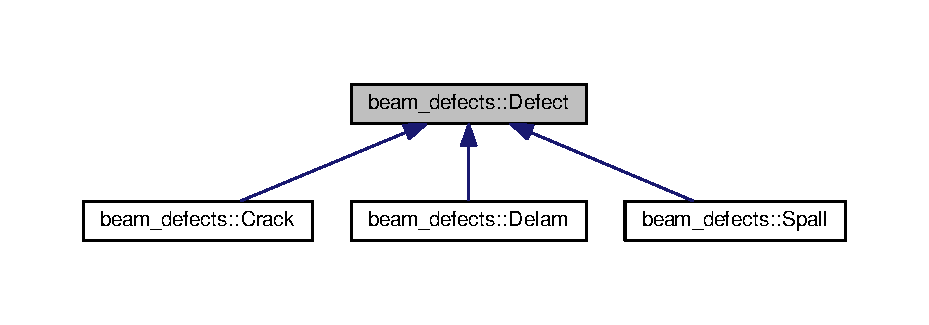
\includegraphics[width=350pt]{classbeam__defects_1_1_defect__inherit__graph}
\end{center}
\end{figure}
\subsection*{Public Types}
\begin{DoxyCompactItemize}
\item 
using \hyperlink{classbeam__defects_1_1_defect_a0a7708c6cd92ac482d45ef606d598325}{Ptr} = std\+::shared\+\_\+ptr$<$ \hyperlink{classbeam__defects_1_1_defect}{Defect} $>$
\end{DoxyCompactItemize}
\subsection*{Public Member Functions}
\begin{DoxyCompactItemize}
\item 
\hyperlink{classbeam__defects_1_1_defect_a3554dc33d88356193000174580bcc41a}{Defect} ()=default
\begin{DoxyCompactList}\small\item\em Default constructor. \end{DoxyCompactList}\item 
virtual \hyperlink{classbeam__defects_1_1_defect_aae70bb9ef052129a6bfc6b6d0de373b9}{$\sim$\+Defect} ()=default
\begin{DoxyCompactList}\small\item\em Default destructor. \end{DoxyCompactList}\item 
virtual double \hyperlink{classbeam__defects_1_1_defect_aa7c24d68d22e6d47dc1b9e8a9ad94c56}{Get\+Size} ()=0
\begin{DoxyCompactList}\small\item\em Pure virtual method for returning the size of a defect. \end{DoxyCompactList}\item 
virtual \hyperlink{group__defects_gae379b271bd5fb7ce92afe1abee917249}{Defect\+Type} \hyperlink{classbeam__defects_1_1_defect_aab237fd856c7ace882ead216c81574e6}{Get\+Type} () const =0
\begin{DoxyCompactList}\small\item\em Pure virtual method for returning type of defect. \end{DoxyCompactList}\item 
virtual \hyperlink{group__defects_gaed38c449f8cba57f35d1af04496a0711}{Defect\+O\+S\+I\+M\+Severity} \hyperlink{classbeam__defects_1_1_defect_a74824cc5cdb9d301d72089585ed8f1f2}{Get\+O\+S\+I\+M\+Severity} ()=0
\end{DoxyCompactItemize}


\subsection{Detailed Description}
Abstract class for defects. 

Definition at line 34 of file Defect.\+h.



\subsection{Member Typedef Documentation}
\index{beam\+\_\+defects\+::\+Defect@{beam\+\_\+defects\+::\+Defect}!Ptr@{Ptr}}
\index{Ptr@{Ptr}!beam\+\_\+defects\+::\+Defect@{beam\+\_\+defects\+::\+Defect}}
\subsubsection[{\texorpdfstring{Ptr}{Ptr}}]{\setlength{\rightskip}{0pt plus 5cm}using {\bf beam\+\_\+defects\+::\+Defect\+::\+Ptr} =  std\+::shared\+\_\+ptr$<${\bf Defect}$>$}\hypertarget{classbeam__defects_1_1_defect_a0a7708c6cd92ac482d45ef606d598325}{}\label{classbeam__defects_1_1_defect_a0a7708c6cd92ac482d45ef606d598325}


Definition at line 60 of file Defect.\+h.



\subsection{Constructor \& Destructor Documentation}
\index{beam\+\_\+defects\+::\+Defect@{beam\+\_\+defects\+::\+Defect}!Defect@{Defect}}
\index{Defect@{Defect}!beam\+\_\+defects\+::\+Defect@{beam\+\_\+defects\+::\+Defect}}
\subsubsection[{\texorpdfstring{Defect()=default}{Defect()=default}}]{\setlength{\rightskip}{0pt plus 5cm}beam\+\_\+defects\+::\+Defect\+::\+Defect (
\begin{DoxyParamCaption}
{}
\end{DoxyParamCaption}
)\hspace{0.3cm}{\ttfamily [default]}}\hypertarget{classbeam__defects_1_1_defect_a3554dc33d88356193000174580bcc41a}{}\label{classbeam__defects_1_1_defect_a3554dc33d88356193000174580bcc41a}


Default constructor. 

\index{beam\+\_\+defects\+::\+Defect@{beam\+\_\+defects\+::\+Defect}!````~Defect@{$\sim$\+Defect}}
\index{````~Defect@{$\sim$\+Defect}!beam\+\_\+defects\+::\+Defect@{beam\+\_\+defects\+::\+Defect}}
\subsubsection[{\texorpdfstring{$\sim$\+Defect()=default}{~Defect()=default}}]{\setlength{\rightskip}{0pt plus 5cm}virtual beam\+\_\+defects\+::\+Defect\+::$\sim$\+Defect (
\begin{DoxyParamCaption}
{}
\end{DoxyParamCaption}
)\hspace{0.3cm}{\ttfamily [virtual]}, {\ttfamily [default]}}\hypertarget{classbeam__defects_1_1_defect_aae70bb9ef052129a6bfc6b6d0de373b9}{}\label{classbeam__defects_1_1_defect_aae70bb9ef052129a6bfc6b6d0de373b9}


Default destructor. 



\subsection{Member Function Documentation}
\index{beam\+\_\+defects\+::\+Defect@{beam\+\_\+defects\+::\+Defect}!Get\+O\+S\+I\+M\+Severity@{Get\+O\+S\+I\+M\+Severity}}
\index{Get\+O\+S\+I\+M\+Severity@{Get\+O\+S\+I\+M\+Severity}!beam\+\_\+defects\+::\+Defect@{beam\+\_\+defects\+::\+Defect}}
\subsubsection[{\texorpdfstring{Get\+O\+S\+I\+M\+Severity()=0}{GetOSIMSeverity()=0}}]{\setlength{\rightskip}{0pt plus 5cm}virtual {\bf Defect\+O\+S\+I\+M\+Severity} beam\+\_\+defects\+::\+Defect\+::\+Get\+O\+S\+I\+M\+Severity (
\begin{DoxyParamCaption}
{}
\end{DoxyParamCaption}
)\hspace{0.3cm}{\ttfamily [pure virtual]}}\hypertarget{classbeam__defects_1_1_defect_a74824cc5cdb9d301d72089585ed8f1f2}{}\label{classbeam__defects_1_1_defect_a74824cc5cdb9d301d72089585ed8f1f2}


Implemented in \hyperlink{classbeam__defects_1_1_crack_a55b689875191ba9049134456d4d2889b}{beam\+\_\+defects\+::\+Crack}, \hyperlink{classbeam__defects_1_1_delam_a185b2cb8f43376dda9a1c87a41e18829}{beam\+\_\+defects\+::\+Delam}, and \hyperlink{classbeam__defects_1_1_spall_a96f74134abee749d37cf750119098c4c}{beam\+\_\+defects\+::\+Spall}.

\index{beam\+\_\+defects\+::\+Defect@{beam\+\_\+defects\+::\+Defect}!Get\+Size@{Get\+Size}}
\index{Get\+Size@{Get\+Size}!beam\+\_\+defects\+::\+Defect@{beam\+\_\+defects\+::\+Defect}}
\subsubsection[{\texorpdfstring{Get\+Size()=0}{GetSize()=0}}]{\setlength{\rightskip}{0pt plus 5cm}virtual double beam\+\_\+defects\+::\+Defect\+::\+Get\+Size (
\begin{DoxyParamCaption}
{}
\end{DoxyParamCaption}
)\hspace{0.3cm}{\ttfamily [pure virtual]}}\hypertarget{classbeam__defects_1_1_defect_aa7c24d68d22e6d47dc1b9e8a9ad94c56}{}\label{classbeam__defects_1_1_defect_aa7c24d68d22e6d47dc1b9e8a9ad94c56}


Pure virtual method for returning the size of a defect. 

\begin{DoxyReturn}{Returns}
Returns size of defect 
\end{DoxyReturn}


Implemented in \hyperlink{classbeam__defects_1_1_crack_a140c08ad86be9062cf4c9b0bfe686d67}{beam\+\_\+defects\+::\+Crack}, \hyperlink{classbeam__defects_1_1_delam_a9a44051492d76e180e85e31724acc26a}{beam\+\_\+defects\+::\+Delam}, and \hyperlink{classbeam__defects_1_1_spall_a84f5aaa8ced3ae1c61eb8f77e540c466}{beam\+\_\+defects\+::\+Spall}.

\index{beam\+\_\+defects\+::\+Defect@{beam\+\_\+defects\+::\+Defect}!Get\+Type@{Get\+Type}}
\index{Get\+Type@{Get\+Type}!beam\+\_\+defects\+::\+Defect@{beam\+\_\+defects\+::\+Defect}}
\subsubsection[{\texorpdfstring{Get\+Type() const =0}{GetType() const =0}}]{\setlength{\rightskip}{0pt plus 5cm}virtual {\bf Defect\+Type} beam\+\_\+defects\+::\+Defect\+::\+Get\+Type (
\begin{DoxyParamCaption}
{}
\end{DoxyParamCaption}
) const\hspace{0.3cm}{\ttfamily [pure virtual]}}\hypertarget{classbeam__defects_1_1_defect_aab237fd856c7ace882ead216c81574e6}{}\label{classbeam__defects_1_1_defect_aab237fd856c7ace882ead216c81574e6}


Pure virtual method for returning type of defect. 

\begin{DoxyReturn}{Returns}

\end{DoxyReturn}


Implemented in \hyperlink{classbeam__defects_1_1_crack_a1f6ede9707c63376e6d409b388770c07}{beam\+\_\+defects\+::\+Crack}, \hyperlink{classbeam__defects_1_1_delam_a098488b1a71796df7e9a6d0eb5eaeeea}{beam\+\_\+defects\+::\+Delam}, and \hyperlink{classbeam__defects_1_1_spall_a98572b81bfd78594f1e497758946aaa1}{beam\+\_\+defects\+::\+Spall}.



The documentation for this class was generated from the following file\+:\begin{DoxyCompactItemize}
\item 
beam\+\_\+defects/include/beam\+\_\+defects/\hyperlink{_defect_8h}{Defect.\+h}\end{DoxyCompactItemize}

\hypertarget{classbeam__defects_1_1_delam}{}\section{beam\+\_\+defects\+:\+:Delam Class Reference}
\label{classbeam__defects_1_1_delam}\index{beam\+\_\+defects\+::\+Delam@{beam\+\_\+defects\+::\+Delam}}


Derived class for delamination defects.  




{\ttfamily \#include $<$Delam.\+h$>$}



Inheritance diagram for beam\+\_\+defects\+:\+:Delam\+:\nopagebreak
\begin{figure}[H]
\begin{center}
\leavevmode
\includegraphics[width=193pt]{classbeam__defects_1_1_delam__inherit__graph}
\end{center}
\end{figure}


Collaboration diagram for beam\+\_\+defects\+:\+:Delam\+:\nopagebreak
\begin{figure}[H]
\begin{center}
\leavevmode
\includegraphics[width=193pt]{classbeam__defects_1_1_delam__coll__graph}
\end{center}
\end{figure}
\subsection*{Public Member Functions}
\begin{DoxyCompactItemize}
\item 
\hyperlink{classbeam__defects_1_1_delam_a1a108358cf5f4d07cbe4ad3b7ac00997}{Delam} ()=default
\begin{DoxyCompactList}\small\item\em Default constructor. \end{DoxyCompactList}\item 
\hyperlink{classbeam__defects_1_1_delam_a985ea836e28343406faa18c173b106c7}{Delam} (pcl\+::\+Point\+Cloud$<$ pcl\+::\+Point\+X\+YZ $>$\+::\hyperlink{classbeam__defects_1_1_defect_a0a7708c6cd92ac482d45ef606d598325}{Ptr} pc)
\begin{DoxyCompactList}\small\item\em Construct with a point cloud. \end{DoxyCompactList}\item 
\hyperlink{classbeam__defects_1_1_delam_aef2a99b590cef7c0b400695ca14533cf}{$\sim$\+Delam} () override=default
\begin{DoxyCompactList}\small\item\em Default constructor. \end{DoxyCompactList}\item 
\hyperlink{group__defects_gae379b271bd5fb7ce92afe1abee917249}{Defect\+Type} \hyperlink{classbeam__defects_1_1_delam_a098488b1a71796df7e9a6d0eb5eaeeea}{Get\+Type} () const override
\begin{DoxyCompactList}\small\item\em Get the type of defect. \end{DoxyCompactList}\item 
double \hyperlink{classbeam__defects_1_1_delam_a9a44051492d76e180e85e31724acc26a}{Get\+Size} () override
\begin{DoxyCompactList}\small\item\em Get the size of the defect. \end{DoxyCompactList}\item 
\hyperlink{group__defects_gaed38c449f8cba57f35d1af04496a0711}{Defect\+O\+S\+I\+M\+Severity} \hyperlink{classbeam__defects_1_1_delam_a185b2cb8f43376dda9a1c87a41e18829}{Get\+O\+S\+I\+M\+Severity} () override
\end{DoxyCompactItemize}
\subsection*{Additional Inherited Members}


\subsection{Detailed Description}
Derived class for delamination defects. 

Definition at line 15 of file Delam.\+h.



\subsection{Constructor \& Destructor Documentation}
\index{beam\+\_\+defects\+::\+Delam@{beam\+\_\+defects\+::\+Delam}!Delam@{Delam}}
\index{Delam@{Delam}!beam\+\_\+defects\+::\+Delam@{beam\+\_\+defects\+::\+Delam}}
\subsubsection[{\texorpdfstring{Delam()=default}{Delam()=default}}]{\setlength{\rightskip}{0pt plus 5cm}beam\+\_\+defects\+::\+Delam\+::\+Delam (
\begin{DoxyParamCaption}
{}
\end{DoxyParamCaption}
)\hspace{0.3cm}{\ttfamily [default]}}\hypertarget{classbeam__defects_1_1_delam_a1a108358cf5f4d07cbe4ad3b7ac00997}{}\label{classbeam__defects_1_1_delam_a1a108358cf5f4d07cbe4ad3b7ac00997}


Default constructor. 

\index{beam\+\_\+defects\+::\+Delam@{beam\+\_\+defects\+::\+Delam}!Delam@{Delam}}
\index{Delam@{Delam}!beam\+\_\+defects\+::\+Delam@{beam\+\_\+defects\+::\+Delam}}
\subsubsection[{\texorpdfstring{Delam(pcl\+::\+Point\+Cloud$<$ pcl\+::\+Point\+X\+Y\+Z $>$\+::\+Ptr pc)}{Delam(pcl::PointCloud< pcl::PointXYZ >::Ptr pc)}}]{\setlength{\rightskip}{0pt plus 5cm}beam\+\_\+defects\+::\+Delam\+::\+Delam (
\begin{DoxyParamCaption}
\item[{pcl\+::\+Point\+Cloud$<$ pcl\+::\+Point\+X\+YZ $>$\+::{\bf Ptr}}]{pc}
\end{DoxyParamCaption}
)\hspace{0.3cm}{\ttfamily [explicit]}}\hypertarget{classbeam__defects_1_1_delam_a985ea836e28343406faa18c173b106c7}{}\label{classbeam__defects_1_1_delam_a985ea836e28343406faa18c173b106c7}


Construct with a point cloud. 


\begin{DoxyParams}{Parameters}
{\em pc} & \\
\hline
\end{DoxyParams}


Definition at line 6 of file Delam.\+cpp.

\index{beam\+\_\+defects\+::\+Delam@{beam\+\_\+defects\+::\+Delam}!````~Delam@{$\sim$\+Delam}}
\index{````~Delam@{$\sim$\+Delam}!beam\+\_\+defects\+::\+Delam@{beam\+\_\+defects\+::\+Delam}}
\subsubsection[{\texorpdfstring{$\sim$\+Delam() override=default}{~Delam() override=default}}]{\setlength{\rightskip}{0pt plus 5cm}beam\+\_\+defects\+::\+Delam\+::$\sim$\+Delam (
\begin{DoxyParamCaption}
{}
\end{DoxyParamCaption}
)\hspace{0.3cm}{\ttfamily [override]}, {\ttfamily [default]}}\hypertarget{classbeam__defects_1_1_delam_aef2a99b590cef7c0b400695ca14533cf}{}\label{classbeam__defects_1_1_delam_aef2a99b590cef7c0b400695ca14533cf}


Default constructor. 



\subsection{Member Function Documentation}
\index{beam\+\_\+defects\+::\+Delam@{beam\+\_\+defects\+::\+Delam}!Get\+O\+S\+I\+M\+Severity@{Get\+O\+S\+I\+M\+Severity}}
\index{Get\+O\+S\+I\+M\+Severity@{Get\+O\+S\+I\+M\+Severity}!beam\+\_\+defects\+::\+Delam@{beam\+\_\+defects\+::\+Delam}}
\subsubsection[{\texorpdfstring{Get\+O\+S\+I\+M\+Severity() override}{GetOSIMSeverity() override}}]{\setlength{\rightskip}{0pt plus 5cm}{\bf Defect\+O\+S\+I\+M\+Severity} beam\+\_\+defects\+::\+Delam\+::\+Get\+O\+S\+I\+M\+Severity (
\begin{DoxyParamCaption}
{}
\end{DoxyParamCaption}
)\hspace{0.3cm}{\ttfamily [override]}, {\ttfamily [virtual]}}\hypertarget{classbeam__defects_1_1_delam_a185b2cb8f43376dda9a1c87a41e18829}{}\label{classbeam__defects_1_1_delam_a185b2cb8f43376dda9a1c87a41e18829}


Implements \hyperlink{classbeam__defects_1_1_defect_a74824cc5cdb9d301d72089585ed8f1f2}{beam\+\_\+defects\+::\+Defect}.



Definition at line 28 of file Delam.\+cpp.

\index{beam\+\_\+defects\+::\+Delam@{beam\+\_\+defects\+::\+Delam}!Get\+Size@{Get\+Size}}
\index{Get\+Size@{Get\+Size}!beam\+\_\+defects\+::\+Delam@{beam\+\_\+defects\+::\+Delam}}
\subsubsection[{\texorpdfstring{Get\+Size() override}{GetSize() override}}]{\setlength{\rightskip}{0pt plus 5cm}double beam\+\_\+defects\+::\+Delam\+::\+Get\+Size (
\begin{DoxyParamCaption}
{}
\end{DoxyParamCaption}
)\hspace{0.3cm}{\ttfamily [override]}, {\ttfamily [virtual]}}\hypertarget{classbeam__defects_1_1_delam_a9a44051492d76e180e85e31724acc26a}{}\label{classbeam__defects_1_1_delam_a9a44051492d76e180e85e31724acc26a}


Get the size of the defect. 

\begin{DoxyReturn}{Returns}
Returns the size of the defect in whatever units are relevant for this class of defect 
\end{DoxyReturn}


Implements \hyperlink{classbeam__defects_1_1_defect_aa7c24d68d22e6d47dc1b9e8a9ad94c56}{beam\+\_\+defects\+::\+Defect}.



Definition at line 8 of file Delam.\+cpp.

\index{beam\+\_\+defects\+::\+Delam@{beam\+\_\+defects\+::\+Delam}!Get\+Type@{Get\+Type}}
\index{Get\+Type@{Get\+Type}!beam\+\_\+defects\+::\+Delam@{beam\+\_\+defects\+::\+Delam}}
\subsubsection[{\texorpdfstring{Get\+Type() const override}{GetType() const override}}]{\setlength{\rightskip}{0pt plus 5cm}{\bf Defect\+Type} beam\+\_\+defects\+::\+Delam\+::\+Get\+Type (
\begin{DoxyParamCaption}
{}
\end{DoxyParamCaption}
) const\hspace{0.3cm}{\ttfamily [inline]}, {\ttfamily [override]}, {\ttfamily [virtual]}}\hypertarget{classbeam__defects_1_1_delam_a098488b1a71796df7e9a6d0eb5eaeeea}{}\label{classbeam__defects_1_1_delam_a098488b1a71796df7e9a6d0eb5eaeeea}


Get the type of defect. 

\begin{DoxyReturn}{Returns}
Returns type as one of defects specified in the enum Defect\+Type 
\end{DoxyReturn}


Implements \hyperlink{classbeam__defects_1_1_defect_aab237fd856c7ace882ead216c81574e6}{beam\+\_\+defects\+::\+Defect}.



Definition at line 37 of file Delam.\+h.



The documentation for this class was generated from the following files\+:\begin{DoxyCompactItemize}
\item 
beam\+\_\+defects/include/beam\+\_\+defects/\hyperlink{_delam_8h}{Delam.\+h}\item 
beam\+\_\+defects/src/\hyperlink{_delam_8cpp}{Delam.\+cpp}\end{DoxyCompactItemize}

\hypertarget{classbeam__calibration_1_1_intrinsics}{}\section{beam\+\_\+calibration\+:\+:Intrinsics Class Reference}
\label{classbeam__calibration_1_1_intrinsics}\index{beam\+\_\+calibration\+::\+Intrinsics@{beam\+\_\+calibration\+::\+Intrinsics}}


Abstract class for calibrations.  




{\ttfamily \#include $<$Intrinsics.\+h$>$}



Inheritance diagram for beam\+\_\+calibration\+:\+:Intrinsics\+:\nopagebreak
\begin{figure}[H]
\begin{center}
\leavevmode
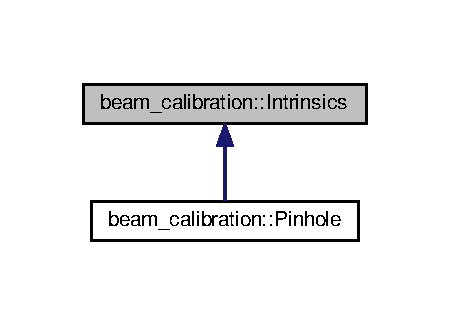
\includegraphics[width=216pt]{classbeam__calibration_1_1_intrinsics__inherit__graph}
\end{center}
\end{figure}
\subsection*{Public Member Functions}
\begin{DoxyCompactItemize}
\item 
\hyperlink{classbeam__calibration_1_1_intrinsics_a383de3546c65f013c8c52b1ed320c8de}{Intrinsics} ()=default
\begin{DoxyCompactList}\small\item\em Default constructor. \end{DoxyCompactList}\item 
virtual \hyperlink{classbeam__calibration_1_1_intrinsics_ac2e5b7bbabb7ed19a1f770925bfac969}{$\sim$\+Intrinsics} ()=default
\begin{DoxyCompactList}\small\item\em Default destructor. \end{DoxyCompactList}\item 
virtual \hyperlink{group__calibration_ga9abafc7bdd7c31c8fdbd4cc90df9a956}{Intrinsics\+Type} \hyperlink{classbeam__calibration_1_1_intrinsics_a4e7f41934491e75c87538e5b6b0caad3}{Get\+Type} () const =0
\begin{DoxyCompactList}\small\item\em Pure virtual method for returning type of intrinsics. \end{DoxyCompactList}\item 
virtual std\+::string \hyperlink{classbeam__calibration_1_1_intrinsics_a77ed2b970f22938699a9a212eb75f7e5}{Get\+Frame\+Id} ()=0
\begin{DoxyCompactList}\small\item\em Pure virtual method for returning the frame id of an intrinsics calibration object. \end{DoxyCompactList}\item 
virtual void \hyperlink{classbeam__calibration_1_1_intrinsics_a713eb2d78358185572e56d922fc3aff2}{Add\+Frame\+Id} (std\+::string frame\+\_\+id)=0
\begin{DoxyCompactList}\small\item\em Pure virtual method for adding the frame id. \end{DoxyCompactList}\item 
virtual \hyperlink{group__utils_ga6112bda54e53755ab14060144285c6b0}{beam\+::\+Vec2} \hyperlink{classbeam__calibration_1_1_intrinsics_a0084b28677b9a242e0f3d8dbaf3ea252}{Get\+Img\+Dims} ()=0
\begin{DoxyCompactList}\small\item\em Pure virtual method for getting the image dimensions. \end{DoxyCompactList}\item 
virtual void \hyperlink{classbeam__calibration_1_1_intrinsics_affd89d4facbec94f8b4ad13ea658c12f}{Add\+Img\+Dims} (\hyperlink{group__utils_ga6112bda54e53755ab14060144285c6b0}{beam\+::\+Vec2} img\+\_\+dims)=0
\begin{DoxyCompactList}\small\item\em Pure virtual method for adding the image dimensions. \end{DoxyCompactList}\end{DoxyCompactItemize}


\subsection{Detailed Description}
Abstract class for calibrations. 

Definition at line 20 of file Intrinsics.\+h.



\subsection{Constructor \& Destructor Documentation}
\index{beam\+\_\+calibration\+::\+Intrinsics@{beam\+\_\+calibration\+::\+Intrinsics}!Intrinsics@{Intrinsics}}
\index{Intrinsics@{Intrinsics}!beam\+\_\+calibration\+::\+Intrinsics@{beam\+\_\+calibration\+::\+Intrinsics}}
\subsubsection[{\texorpdfstring{Intrinsics()=default}{Intrinsics()=default}}]{\setlength{\rightskip}{0pt plus 5cm}beam\+\_\+calibration\+::\+Intrinsics\+::\+Intrinsics (
\begin{DoxyParamCaption}
{}
\end{DoxyParamCaption}
)\hspace{0.3cm}{\ttfamily [default]}}\hypertarget{classbeam__calibration_1_1_intrinsics_a383de3546c65f013c8c52b1ed320c8de}{}\label{classbeam__calibration_1_1_intrinsics_a383de3546c65f013c8c52b1ed320c8de}


Default constructor. 

\index{beam\+\_\+calibration\+::\+Intrinsics@{beam\+\_\+calibration\+::\+Intrinsics}!````~Intrinsics@{$\sim$\+Intrinsics}}
\index{````~Intrinsics@{$\sim$\+Intrinsics}!beam\+\_\+calibration\+::\+Intrinsics@{beam\+\_\+calibration\+::\+Intrinsics}}
\subsubsection[{\texorpdfstring{$\sim$\+Intrinsics()=default}{~Intrinsics()=default}}]{\setlength{\rightskip}{0pt plus 5cm}virtual beam\+\_\+calibration\+::\+Intrinsics\+::$\sim$\+Intrinsics (
\begin{DoxyParamCaption}
{}
\end{DoxyParamCaption}
)\hspace{0.3cm}{\ttfamily [virtual]}, {\ttfamily [default]}}\hypertarget{classbeam__calibration_1_1_intrinsics_ac2e5b7bbabb7ed19a1f770925bfac969}{}\label{classbeam__calibration_1_1_intrinsics_ac2e5b7bbabb7ed19a1f770925bfac969}


Default destructor. 



\subsection{Member Function Documentation}
\index{beam\+\_\+calibration\+::\+Intrinsics@{beam\+\_\+calibration\+::\+Intrinsics}!Add\+Frame\+Id@{Add\+Frame\+Id}}
\index{Add\+Frame\+Id@{Add\+Frame\+Id}!beam\+\_\+calibration\+::\+Intrinsics@{beam\+\_\+calibration\+::\+Intrinsics}}
\subsubsection[{\texorpdfstring{Add\+Frame\+Id(std\+::string frame\+\_\+id)=0}{AddFrameId(std::string frame_id)=0}}]{\setlength{\rightskip}{0pt plus 5cm}virtual void beam\+\_\+calibration\+::\+Intrinsics\+::\+Add\+Frame\+Id (
\begin{DoxyParamCaption}
\item[{std\+::string}]{frame\+\_\+id}
\end{DoxyParamCaption}
)\hspace{0.3cm}{\ttfamily [pure virtual]}}\hypertarget{classbeam__calibration_1_1_intrinsics_a713eb2d78358185572e56d922fc3aff2}{}\label{classbeam__calibration_1_1_intrinsics_a713eb2d78358185572e56d922fc3aff2}


Pure virtual method for adding the frame id. 


\begin{DoxyParams}{Parameters}
{\em frame\+\_\+id} & frame associated with the intrinsics calibration object \\
\hline
\end{DoxyParams}


Implemented in \hyperlink{classbeam__calibration_1_1_pinhole_ae9a7670fe65481cd2b3847d8fd07c7be}{beam\+\_\+calibration\+::\+Pinhole}.

\index{beam\+\_\+calibration\+::\+Intrinsics@{beam\+\_\+calibration\+::\+Intrinsics}!Add\+Img\+Dims@{Add\+Img\+Dims}}
\index{Add\+Img\+Dims@{Add\+Img\+Dims}!beam\+\_\+calibration\+::\+Intrinsics@{beam\+\_\+calibration\+::\+Intrinsics}}
\subsubsection[{\texorpdfstring{Add\+Img\+Dims(beam\+::\+Vec2 img\+\_\+dims)=0}{AddImgDims(beam::Vec2 img_dims)=0}}]{\setlength{\rightskip}{0pt plus 5cm}virtual void beam\+\_\+calibration\+::\+Intrinsics\+::\+Add\+Img\+Dims (
\begin{DoxyParamCaption}
\item[{{\bf beam\+::\+Vec2}}]{img\+\_\+dims}
\end{DoxyParamCaption}
)\hspace{0.3cm}{\ttfamily [pure virtual]}}\hypertarget{classbeam__calibration_1_1_intrinsics_affd89d4facbec94f8b4ad13ea658c12f}{}\label{classbeam__calibration_1_1_intrinsics_affd89d4facbec94f8b4ad13ea658c12f}


Pure virtual method for adding the image dimensions. 


\begin{DoxyParams}{Parameters}
{\em img\+\_\+dims} & dimensions of the images taken by the camera associated with this intrinsics object\+: \mbox{[}height, width\mbox{]}$^\wedge$T \\
\hline
\end{DoxyParams}


Implemented in \hyperlink{classbeam__calibration_1_1_pinhole_a1c4f6b9c07d9b4b99980daa540a7598e}{beam\+\_\+calibration\+::\+Pinhole}.

\index{beam\+\_\+calibration\+::\+Intrinsics@{beam\+\_\+calibration\+::\+Intrinsics}!Get\+Frame\+Id@{Get\+Frame\+Id}}
\index{Get\+Frame\+Id@{Get\+Frame\+Id}!beam\+\_\+calibration\+::\+Intrinsics@{beam\+\_\+calibration\+::\+Intrinsics}}
\subsubsection[{\texorpdfstring{Get\+Frame\+Id()=0}{GetFrameId()=0}}]{\setlength{\rightskip}{0pt plus 5cm}virtual std\+::string beam\+\_\+calibration\+::\+Intrinsics\+::\+Get\+Frame\+Id (
\begin{DoxyParamCaption}
{}
\end{DoxyParamCaption}
)\hspace{0.3cm}{\ttfamily [pure virtual]}}\hypertarget{classbeam__calibration_1_1_intrinsics_a77ed2b970f22938699a9a212eb75f7e5}{}\label{classbeam__calibration_1_1_intrinsics_a77ed2b970f22938699a9a212eb75f7e5}


Pure virtual method for returning the frame id of an intrinsics calibration object. 

\begin{DoxyReturn}{Returns}
Returns frame id 
\end{DoxyReturn}


Implemented in \hyperlink{classbeam__calibration_1_1_pinhole_aa776bdaf5ced5d79175303ad2fa5e281}{beam\+\_\+calibration\+::\+Pinhole}.

\index{beam\+\_\+calibration\+::\+Intrinsics@{beam\+\_\+calibration\+::\+Intrinsics}!Get\+Img\+Dims@{Get\+Img\+Dims}}
\index{Get\+Img\+Dims@{Get\+Img\+Dims}!beam\+\_\+calibration\+::\+Intrinsics@{beam\+\_\+calibration\+::\+Intrinsics}}
\subsubsection[{\texorpdfstring{Get\+Img\+Dims()=0}{GetImgDims()=0}}]{\setlength{\rightskip}{0pt plus 5cm}virtual {\bf beam\+::\+Vec2} beam\+\_\+calibration\+::\+Intrinsics\+::\+Get\+Img\+Dims (
\begin{DoxyParamCaption}
{}
\end{DoxyParamCaption}
)\hspace{0.3cm}{\ttfamily [pure virtual]}}\hypertarget{classbeam__calibration_1_1_intrinsics_a0084b28677b9a242e0f3d8dbaf3ea252}{}\label{classbeam__calibration_1_1_intrinsics_a0084b28677b9a242e0f3d8dbaf3ea252}


Pure virtual method for getting the image dimensions. 

\begin{DoxyReturn}{Returns}
img\+\_\+dims dimensions of the images taken by the camera associated with this intrinsics object\+: \mbox{[}height, width\mbox{]}$^\wedge$T 
\end{DoxyReturn}


Implemented in \hyperlink{classbeam__calibration_1_1_pinhole_a66f72fdaac253195585aa121a37f312e}{beam\+\_\+calibration\+::\+Pinhole}.

\index{beam\+\_\+calibration\+::\+Intrinsics@{beam\+\_\+calibration\+::\+Intrinsics}!Get\+Type@{Get\+Type}}
\index{Get\+Type@{Get\+Type}!beam\+\_\+calibration\+::\+Intrinsics@{beam\+\_\+calibration\+::\+Intrinsics}}
\subsubsection[{\texorpdfstring{Get\+Type() const =0}{GetType() const =0}}]{\setlength{\rightskip}{0pt plus 5cm}virtual {\bf Intrinsics\+Type} beam\+\_\+calibration\+::\+Intrinsics\+::\+Get\+Type (
\begin{DoxyParamCaption}
{}
\end{DoxyParamCaption}
) const\hspace{0.3cm}{\ttfamily [pure virtual]}}\hypertarget{classbeam__calibration_1_1_intrinsics_a4e7f41934491e75c87538e5b6b0caad3}{}\label{classbeam__calibration_1_1_intrinsics_a4e7f41934491e75c87538e5b6b0caad3}


Pure virtual method for returning type of intrinsics. 

\begin{DoxyReturn}{Returns}
type of intrinsics object 
\end{DoxyReturn}


Implemented in \hyperlink{classbeam__calibration_1_1_pinhole_a54dd38a3820f71a5d8b6a753d32da56f}{beam\+\_\+calibration\+::\+Pinhole}.



The documentation for this class was generated from the following file\+:\begin{DoxyCompactItemize}
\item 
beam\+\_\+calibration/include/beam/calibration/\hyperlink{_intrinsics_8h}{Intrinsics.\+h}\end{DoxyCompactItemize}

\hypertarget{structbeam_1_1_mat_comparator}{}\section{beam\+:\+:Mat\+Comparator Struct Reference}
\label{structbeam_1_1_mat_comparator}\index{beam\+::\+Mat\+Comparator@{beam\+::\+Mat\+Comparator}}


{\ttfamily \#include $<$math.\+hpp$>$}

\subsection*{Public Member Functions}
\begin{DoxyCompactItemize}
\item 
bool \hyperlink{structbeam_1_1_mat_comparator_a50750c873205b76d8d86d7349ebde6e3}{operator()} (const \hyperlink{group__utils_gaf1ee9917aef6e6cf513d29f8c7d2eeee}{MatX} \&a, const \hyperlink{group__utils_gaf1ee9917aef6e6cf513d29f8c7d2eeee}{MatX} \&b) const 
\end{DoxyCompactItemize}


\subsection{Detailed Description}
Eigen matrix comparator 

Definition at line 58 of file math.\+hpp.



\subsection{Member Function Documentation}
\index{beam\+::\+Mat\+Comparator@{beam\+::\+Mat\+Comparator}!operator()@{operator()}}
\index{operator()@{operator()}!beam\+::\+Mat\+Comparator@{beam\+::\+Mat\+Comparator}}
\subsubsection[{\texorpdfstring{operator()(const Mat\+X \&a, const Mat\+X \&b) const }{operator()(const MatX &a, const MatX &b) const }}]{\setlength{\rightskip}{0pt plus 5cm}bool beam\+::\+Mat\+Comparator\+::operator() (
\begin{DoxyParamCaption}
\item[{const {\bf MatX} \&}]{a, }
\item[{const {\bf MatX} \&}]{b}
\end{DoxyParamCaption}
) const\hspace{0.3cm}{\ttfamily [inline]}}\hypertarget{structbeam_1_1_mat_comparator_a50750c873205b76d8d86d7349ebde6e3}{}\label{structbeam_1_1_mat_comparator_a50750c873205b76d8d86d7349ebde6e3}


Definition at line 59 of file math.\+hpp.



The documentation for this struct was generated from the following file\+:\begin{DoxyCompactItemize}
\item 
beam\+\_\+utils/include/beam/utils/\hyperlink{math_8hpp}{math.\+hpp}\end{DoxyCompactItemize}

\hypertarget{classbeam__calibration_1_1_pinhole}{}\section{beam\+\_\+calibration\+:\+:Pinhole Class Reference}
\label{classbeam__calibration_1_1_pinhole}\index{beam\+\_\+calibration\+::\+Pinhole@{beam\+\_\+calibration\+::\+Pinhole}}


Derived class for pinhole intrinsics.  




{\ttfamily \#include $<$Pinhole.\+h$>$}



Inheritance diagram for beam\+\_\+calibration\+:\+:Pinhole\+:\nopagebreak
\begin{figure}[H]
\begin{center}
\leavevmode
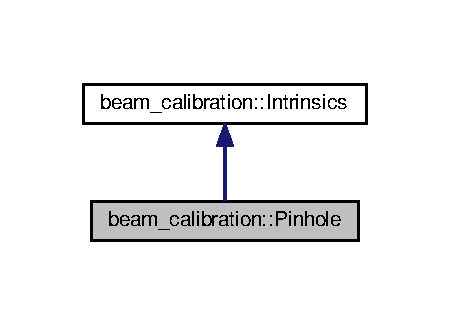
\includegraphics[width=216pt]{classbeam__calibration_1_1_pinhole__inherit__graph}
\end{center}
\end{figure}


Collaboration diagram for beam\+\_\+calibration\+:\+:Pinhole\+:\nopagebreak
\begin{figure}[H]
\begin{center}
\leavevmode
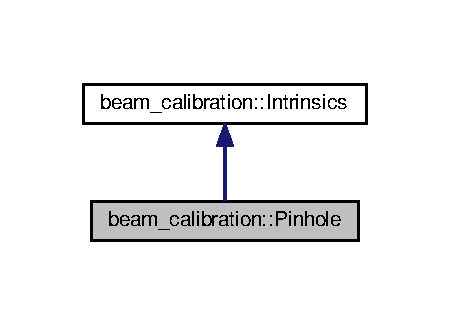
\includegraphics[width=216pt]{classbeam__calibration_1_1_pinhole__coll__graph}
\end{center}
\end{figure}
\subsection*{Public Member Functions}
\begin{DoxyCompactItemize}
\item 
\hyperlink{classbeam__calibration_1_1_pinhole_abba8b5c4d7d467b4137802dc1221cf5c}{Pinhole} ()=default
\begin{DoxyCompactList}\small\item\em Default constructor. \end{DoxyCompactList}\item 
\hyperlink{classbeam__calibration_1_1_pinhole_aafd4e22eac71beed825c306981a4a59a}{Pinhole} (double fx, double fy, double cx, double cy)
\begin{DoxyCompactList}\small\item\em constructor \end{DoxyCompactList}\item 
\hyperlink{classbeam__calibration_1_1_pinhole_a63dd0e2c171429a6b6e9a69c13b273ed}{Pinhole} (\hyperlink{group__utils_ga665fed2673de952d12b19351a2bdb961}{beam\+::\+Mat3} K)
\begin{DoxyCompactList}\small\item\em constructor \end{DoxyCompactList}\item 
\hyperlink{classbeam__calibration_1_1_pinhole_a42abf55373c49f0ce0a44535498e1c33}{$\sim$\+Pinhole} () override=default
\begin{DoxyCompactList}\small\item\em Default constructor. \end{DoxyCompactList}\item 
\hyperlink{group__calibration_ga9abafc7bdd7c31c8fdbd4cc90df9a956}{Intrinsics\+Type} \hyperlink{classbeam__calibration_1_1_pinhole_a54dd38a3820f71a5d8b6a753d32da56f}{Get\+Type} () const override
\begin{DoxyCompactList}\small\item\em Get the type of intrinsic. \end{DoxyCompactList}\item 
void \hyperlink{classbeam__calibration_1_1_pinhole_ae9a7670fe65481cd2b3847d8fd07c7be}{Add\+Frame\+Id} (std\+::string frame\+\_\+id) override
\begin{DoxyCompactList}\small\item\em Method for adding the frame id. \end{DoxyCompactList}\item 
std\+::string \hyperlink{classbeam__calibration_1_1_pinhole_aa776bdaf5ced5d79175303ad2fa5e281}{Get\+Frame\+Id} () override
\begin{DoxyCompactList}\small\item\em Method for returning the frame id of an intrinsics calibration object. \end{DoxyCompactList}\item 
void \hyperlink{classbeam__calibration_1_1_pinhole_a1c4f6b9c07d9b4b99980daa540a7598e}{Add\+Img\+Dims} (\hyperlink{group__utils_ga6112bda54e53755ab14060144285c6b0}{beam\+::\+Vec2} img\+\_\+dims) override
\begin{DoxyCompactList}\small\item\em Method for adding the image dimensions. \end{DoxyCompactList}\item 
\hyperlink{group__utils_ga6112bda54e53755ab14060144285c6b0}{beam\+::\+Vec2} \hyperlink{classbeam__calibration_1_1_pinhole_a66f72fdaac253195585aa121a37f312e}{Get\+Img\+Dims} () override
\begin{DoxyCompactList}\small\item\em Method for getting the image dimensions. \end{DoxyCompactList}\item 
\hyperlink{group__utils_ga665fed2673de952d12b19351a2bdb961}{beam\+::\+Mat3} \hyperlink{classbeam__calibration_1_1_pinhole_a0d004fb525f086ccc9cb46822fbe5c4e}{GetK} ()
\begin{DoxyCompactList}\small\item\em Method for returning K matrix. \end{DoxyCompactList}\item 
double \hyperlink{classbeam__calibration_1_1_pinhole_a75f59db7472104970ec6063989c5d2ad}{Get\+Fy} ()
\begin{DoxyCompactList}\small\item\em Method for returning y focal length. \end{DoxyCompactList}\item 
double \hyperlink{classbeam__calibration_1_1_pinhole_afdf888a775d106d6a618c0a93b6f1109}{Get\+Fx} ()
\begin{DoxyCompactList}\small\item\em Method for returning x focal length. \end{DoxyCompactList}\item 
double \hyperlink{classbeam__calibration_1_1_pinhole_ae76ebf82800677949ba90179393eeefa}{Get\+Cx} ()
\begin{DoxyCompactList}\small\item\em Method for returning optical center in x direction. \end{DoxyCompactList}\item 
double \hyperlink{classbeam__calibration_1_1_pinhole_a7fcb0a42c56369c920f56251c6451b59}{Get\+Cy} ()
\begin{DoxyCompactList}\small\item\em Method for returning optical center in y direction. \end{DoxyCompactList}\item 
bool \hyperlink{classbeam__calibration_1_1_pinhole_a326e7bb0ae15aea808d7f11c6c706869}{Is\+Full} ()
\begin{DoxyCompactList}\small\item\em Method for checking if the intinsic parameters have been set. \end{DoxyCompactList}\item 
void \hyperlink{classbeam__calibration_1_1_pinhole_a6d0bc4ac42aeb376a7138065b8ca7ade}{Add\+Tan\+Dist} (\hyperlink{group__utils_ga6112bda54e53755ab14060144285c6b0}{beam\+::\+Vec2} tan\+\_\+coeffs)
\begin{DoxyCompactList}\small\item\em Method for adding tangential distortion parameters. \end{DoxyCompactList}\item 
void \hyperlink{classbeam__calibration_1_1_pinhole_a6bc5e220a93ea3a2b398c5bb443e49d0}{Add\+Rad\+Dist} (\hyperlink{group__utils_gae5ba967e4b0d4b421ca30ef46f896145}{beam\+::\+VecX} rad\+\_\+coeffs)
\begin{DoxyCompactList}\small\item\em Method for adding radial distortion parameters. \end{DoxyCompactList}\item 
\hyperlink{group__utils_ga6112bda54e53755ab14060144285c6b0}{beam\+::\+Vec2} \hyperlink{classbeam__calibration_1_1_pinhole_aee136039482aed25893c2ab37b5c00aa}{Get\+Tan\+Dist} ()
\begin{DoxyCompactList}\small\item\em Method for getting tangential distortion parameters. \end{DoxyCompactList}\item 
\hyperlink{group__utils_gae5ba967e4b0d4b421ca30ef46f896145}{beam\+::\+VecX} \hyperlink{classbeam__calibration_1_1_pinhole_ac455a6e6c46e7dafa14eac53042723d2}{Get\+Rad\+Dist} ()
\begin{DoxyCompactList}\small\item\em Method for getting radial distortion parameters. \end{DoxyCompactList}\item 
\hyperlink{group__utils_ga6112bda54e53755ab14060144285c6b0}{beam\+::\+Vec2} \hyperlink{classbeam__calibration_1_1_pinhole_a4834e766dc9c57b8c2cbc92f21173ebb}{Project\+Point} (\hyperlink{group__utils_ga7aca82b90a74cb643417801e830cd43f}{beam\+::\+Vec3} X)
\begin{DoxyCompactList}\small\item\em Method for projecting a point into an image plane. \end{DoxyCompactList}\item 
\hyperlink{group__utils_ga6112bda54e53755ab14060144285c6b0}{beam\+::\+Vec2} \hyperlink{classbeam__calibration_1_1_pinhole_a71b497379ab57ac3952563f3e0d62e88}{Project\+Point} (\hyperlink{group__utils_gae8c630e8f7e9cdbc1a7dcc3073a99d5c}{beam\+::\+Vec4} X)
\begin{DoxyCompactList}\small\item\em Method for projecting a point in homographic form into an image plane. \end{DoxyCompactList}\item 
\hyperlink{group__utils_ga6112bda54e53755ab14060144285c6b0}{beam\+::\+Vec2} \hyperlink{classbeam__calibration_1_1_pinhole_ade6c53821bc84a8795f5101ff49bfd36}{Project\+Distorted\+Point} (\hyperlink{group__utils_ga7aca82b90a74cb643417801e830cd43f}{beam\+::\+Vec3} X)
\begin{DoxyCompactList}\small\item\em Method for projecting a point into an image plane where the image is distorted. See\+: \href{https://docs.opencv.org/2.4/modules/calib3d/doc/camera_calibration_and_3d_reconstruction.html}{\tt https\+://docs.\+opencv.\+org/2.\+4/modules/calib3d/doc/camera\+\_\+calibration\+\_\+and\+\_\+3d\+\_\+reconstruction.\+html}. \end{DoxyCompactList}\item 
\hyperlink{group__utils_ga6112bda54e53755ab14060144285c6b0}{beam\+::\+Vec2} \hyperlink{classbeam__calibration_1_1_pinhole_a101b14c95d8ca7c73c0f4de01dd6605e}{Project\+Distorted\+Point} (\hyperlink{group__utils_gae8c630e8f7e9cdbc1a7dcc3073a99d5c}{beam\+::\+Vec4} X)
\begin{DoxyCompactList}\small\item\em Method for projecting a point in homographic form into an image plane where the image is distorted. See\+: \href{https://docs.opencv.org/2.4/modules/calib3d/doc/camera_calibration_and_3d_reconstruction.html}{\tt https\+://docs.\+opencv.\+org/2.\+4/modules/calib3d/doc/camera\+\_\+calibration\+\_\+and\+\_\+3d\+\_\+reconstruction.\+html}. \end{DoxyCompactList}\end{DoxyCompactItemize}


\subsection{Detailed Description}
Derived class for pinhole intrinsics. 

Definition at line 16 of file Pinhole.\+h.



\subsection{Constructor \& Destructor Documentation}
\index{beam\+\_\+calibration\+::\+Pinhole@{beam\+\_\+calibration\+::\+Pinhole}!Pinhole@{Pinhole}}
\index{Pinhole@{Pinhole}!beam\+\_\+calibration\+::\+Pinhole@{beam\+\_\+calibration\+::\+Pinhole}}
\subsubsection[{\texorpdfstring{Pinhole()=default}{Pinhole()=default}}]{\setlength{\rightskip}{0pt plus 5cm}beam\+\_\+calibration\+::\+Pinhole\+::\+Pinhole (
\begin{DoxyParamCaption}
{}
\end{DoxyParamCaption}
)\hspace{0.3cm}{\ttfamily [default]}}\hypertarget{classbeam__calibration_1_1_pinhole_abba8b5c4d7d467b4137802dc1221cf5c}{}\label{classbeam__calibration_1_1_pinhole_abba8b5c4d7d467b4137802dc1221cf5c}


Default constructor. 

\index{beam\+\_\+calibration\+::\+Pinhole@{beam\+\_\+calibration\+::\+Pinhole}!Pinhole@{Pinhole}}
\index{Pinhole@{Pinhole}!beam\+\_\+calibration\+::\+Pinhole@{beam\+\_\+calibration\+::\+Pinhole}}
\subsubsection[{\texorpdfstring{Pinhole(double fx, double fy, double cx, double cy)}{Pinhole(double fx, double fy, double cx, double cy)}}]{\setlength{\rightskip}{0pt plus 5cm}beam\+\_\+calibration\+::\+Pinhole\+::\+Pinhole (
\begin{DoxyParamCaption}
\item[{double}]{fx, }
\item[{double}]{fy, }
\item[{double}]{cx, }
\item[{double}]{cy}
\end{DoxyParamCaption}
)}\hypertarget{classbeam__calibration_1_1_pinhole_aafd4e22eac71beed825c306981a4a59a}{}\label{classbeam__calibration_1_1_pinhole_aafd4e22eac71beed825c306981a4a59a}


constructor 



Definition at line 7 of file Pinhole.\+cpp.

\index{beam\+\_\+calibration\+::\+Pinhole@{beam\+\_\+calibration\+::\+Pinhole}!Pinhole@{Pinhole}}
\index{Pinhole@{Pinhole}!beam\+\_\+calibration\+::\+Pinhole@{beam\+\_\+calibration\+::\+Pinhole}}
\subsubsection[{\texorpdfstring{Pinhole(beam\+::\+Mat3 K)}{Pinhole(beam::Mat3 K)}}]{\setlength{\rightskip}{0pt plus 5cm}beam\+\_\+calibration\+::\+Pinhole\+::\+Pinhole (
\begin{DoxyParamCaption}
\item[{{\bf beam\+::\+Mat3}}]{K}
\end{DoxyParamCaption}
)}\hypertarget{classbeam__calibration_1_1_pinhole_a63dd0e2c171429a6b6e9a69c13b273ed}{}\label{classbeam__calibration_1_1_pinhole_a63dd0e2c171429a6b6e9a69c13b273ed}


constructor 



Definition at line 12 of file Pinhole.\+cpp.

\index{beam\+\_\+calibration\+::\+Pinhole@{beam\+\_\+calibration\+::\+Pinhole}!````~Pinhole@{$\sim$\+Pinhole}}
\index{````~Pinhole@{$\sim$\+Pinhole}!beam\+\_\+calibration\+::\+Pinhole@{beam\+\_\+calibration\+::\+Pinhole}}
\subsubsection[{\texorpdfstring{$\sim$\+Pinhole() override=default}{~Pinhole() override=default}}]{\setlength{\rightskip}{0pt plus 5cm}beam\+\_\+calibration\+::\+Pinhole\+::$\sim$\+Pinhole (
\begin{DoxyParamCaption}
{}
\end{DoxyParamCaption}
)\hspace{0.3cm}{\ttfamily [override]}, {\ttfamily [default]}}\hypertarget{classbeam__calibration_1_1_pinhole_a42abf55373c49f0ce0a44535498e1c33}{}\label{classbeam__calibration_1_1_pinhole_a42abf55373c49f0ce0a44535498e1c33}


Default constructor. 



\subsection{Member Function Documentation}
\index{beam\+\_\+calibration\+::\+Pinhole@{beam\+\_\+calibration\+::\+Pinhole}!Add\+Frame\+Id@{Add\+Frame\+Id}}
\index{Add\+Frame\+Id@{Add\+Frame\+Id}!beam\+\_\+calibration\+::\+Pinhole@{beam\+\_\+calibration\+::\+Pinhole}}
\subsubsection[{\texorpdfstring{Add\+Frame\+Id(std\+::string frame\+\_\+id) override}{AddFrameId(std::string frame_id) override}}]{\setlength{\rightskip}{0pt plus 5cm}void beam\+\_\+calibration\+::\+Pinhole\+::\+Add\+Frame\+Id (
\begin{DoxyParamCaption}
\item[{std\+::string}]{frame\+\_\+id}
\end{DoxyParamCaption}
)\hspace{0.3cm}{\ttfamily [override]}, {\ttfamily [virtual]}}\hypertarget{classbeam__calibration_1_1_pinhole_ae9a7670fe65481cd2b3847d8fd07c7be}{}\label{classbeam__calibration_1_1_pinhole_ae9a7670fe65481cd2b3847d8fd07c7be}


Method for adding the frame id. 


\begin{DoxyParams}{Parameters}
{\em frame\+\_\+id} & frame associated with the intrinsics calibration object \\
\hline
\end{DoxyParams}


Implements \hyperlink{classbeam__calibration_1_1_intrinsics_a713eb2d78358185572e56d922fc3aff2}{beam\+\_\+calibration\+::\+Intrinsics}.



Definition at line 22 of file Pinhole.\+cpp.

\index{beam\+\_\+calibration\+::\+Pinhole@{beam\+\_\+calibration\+::\+Pinhole}!Add\+Img\+Dims@{Add\+Img\+Dims}}
\index{Add\+Img\+Dims@{Add\+Img\+Dims}!beam\+\_\+calibration\+::\+Pinhole@{beam\+\_\+calibration\+::\+Pinhole}}
\subsubsection[{\texorpdfstring{Add\+Img\+Dims(beam\+::\+Vec2 img\+\_\+dims) override}{AddImgDims(beam::Vec2 img_dims) override}}]{\setlength{\rightskip}{0pt plus 5cm}void beam\+\_\+calibration\+::\+Pinhole\+::\+Add\+Img\+Dims (
\begin{DoxyParamCaption}
\item[{{\bf beam\+::\+Vec2}}]{img\+\_\+dims}
\end{DoxyParamCaption}
)\hspace{0.3cm}{\ttfamily [override]}, {\ttfamily [virtual]}}\hypertarget{classbeam__calibration_1_1_pinhole_a1c4f6b9c07d9b4b99980daa540a7598e}{}\label{classbeam__calibration_1_1_pinhole_a1c4f6b9c07d9b4b99980daa540a7598e}


Method for adding the image dimensions. 


\begin{DoxyParams}{Parameters}
{\em img\+\_\+dims} & dimensions of the images taken by the camera associated with this intrinsics object\+: \mbox{[}height, width\mbox{]}$^\wedge$T \\
\hline
\end{DoxyParams}


Implements \hyperlink{classbeam__calibration_1_1_intrinsics_affd89d4facbec94f8b4ad13ea658c12f}{beam\+\_\+calibration\+::\+Intrinsics}.



Definition at line 30 of file Pinhole.\+cpp.

\index{beam\+\_\+calibration\+::\+Pinhole@{beam\+\_\+calibration\+::\+Pinhole}!Add\+Rad\+Dist@{Add\+Rad\+Dist}}
\index{Add\+Rad\+Dist@{Add\+Rad\+Dist}!beam\+\_\+calibration\+::\+Pinhole@{beam\+\_\+calibration\+::\+Pinhole}}
\subsubsection[{\texorpdfstring{Add\+Rad\+Dist(beam\+::\+Vec\+X rad\+\_\+coeffs)}{AddRadDist(beam::VecX rad_coeffs)}}]{\setlength{\rightskip}{0pt plus 5cm}void beam\+\_\+calibration\+::\+Pinhole\+::\+Add\+Rad\+Dist (
\begin{DoxyParamCaption}
\item[{{\bf beam\+::\+VecX}}]{rad\+\_\+coeffs}
\end{DoxyParamCaption}
)}\hypertarget{classbeam__calibration_1_1_pinhole_a6bc5e220a93ea3a2b398c5bb443e49d0}{}\label{classbeam__calibration_1_1_pinhole_a6bc5e220a93ea3a2b398c5bb443e49d0}


Method for adding radial distortion parameters. 



Definition at line 67 of file Pinhole.\+cpp.

\index{beam\+\_\+calibration\+::\+Pinhole@{beam\+\_\+calibration\+::\+Pinhole}!Add\+Tan\+Dist@{Add\+Tan\+Dist}}
\index{Add\+Tan\+Dist@{Add\+Tan\+Dist}!beam\+\_\+calibration\+::\+Pinhole@{beam\+\_\+calibration\+::\+Pinhole}}
\subsubsection[{\texorpdfstring{Add\+Tan\+Dist(beam\+::\+Vec2 tan\+\_\+coeffs)}{AddTanDist(beam::Vec2 tan_coeffs)}}]{\setlength{\rightskip}{0pt plus 5cm}void beam\+\_\+calibration\+::\+Pinhole\+::\+Add\+Tan\+Dist (
\begin{DoxyParamCaption}
\item[{{\bf beam\+::\+Vec2}}]{tan\+\_\+coeffs}
\end{DoxyParamCaption}
)}\hypertarget{classbeam__calibration_1_1_pinhole_a6d0bc4ac42aeb376a7138065b8ca7ade}{}\label{classbeam__calibration_1_1_pinhole_a6d0bc4ac42aeb376a7138065b8ca7ade}


Method for adding tangential distortion parameters. 



Definition at line 62 of file Pinhole.\+cpp.

\index{beam\+\_\+calibration\+::\+Pinhole@{beam\+\_\+calibration\+::\+Pinhole}!Get\+Cx@{Get\+Cx}}
\index{Get\+Cx@{Get\+Cx}!beam\+\_\+calibration\+::\+Pinhole@{beam\+\_\+calibration\+::\+Pinhole}}
\subsubsection[{\texorpdfstring{Get\+Cx()}{GetCx()}}]{\setlength{\rightskip}{0pt plus 5cm}double beam\+\_\+calibration\+::\+Pinhole\+::\+Get\+Cx (
\begin{DoxyParamCaption}
{}
\end{DoxyParamCaption}
)}\hypertarget{classbeam__calibration_1_1_pinhole_ae76ebf82800677949ba90179393eeefa}{}\label{classbeam__calibration_1_1_pinhole_ae76ebf82800677949ba90179393eeefa}


Method for returning optical center in x direction. 

\begin{DoxyReturn}{Returns}
Cx 
\end{DoxyReturn}


Definition at line 50 of file Pinhole.\+cpp.

\index{beam\+\_\+calibration\+::\+Pinhole@{beam\+\_\+calibration\+::\+Pinhole}!Get\+Cy@{Get\+Cy}}
\index{Get\+Cy@{Get\+Cy}!beam\+\_\+calibration\+::\+Pinhole@{beam\+\_\+calibration\+::\+Pinhole}}
\subsubsection[{\texorpdfstring{Get\+Cy()}{GetCy()}}]{\setlength{\rightskip}{0pt plus 5cm}double beam\+\_\+calibration\+::\+Pinhole\+::\+Get\+Cy (
\begin{DoxyParamCaption}
{}
\end{DoxyParamCaption}
)}\hypertarget{classbeam__calibration_1_1_pinhole_a7fcb0a42c56369c920f56251c6451b59}{}\label{classbeam__calibration_1_1_pinhole_a7fcb0a42c56369c920f56251c6451b59}


Method for returning optical center in y direction. 

\begin{DoxyReturn}{Returns}
Cy 
\end{DoxyReturn}


Definition at line 52 of file Pinhole.\+cpp.

\index{beam\+\_\+calibration\+::\+Pinhole@{beam\+\_\+calibration\+::\+Pinhole}!Get\+Frame\+Id@{Get\+Frame\+Id}}
\index{Get\+Frame\+Id@{Get\+Frame\+Id}!beam\+\_\+calibration\+::\+Pinhole@{beam\+\_\+calibration\+::\+Pinhole}}
\subsubsection[{\texorpdfstring{Get\+Frame\+Id() override}{GetFrameId() override}}]{\setlength{\rightskip}{0pt plus 5cm}std\+::string beam\+\_\+calibration\+::\+Pinhole\+::\+Get\+Frame\+Id (
\begin{DoxyParamCaption}
{}
\end{DoxyParamCaption}
)\hspace{0.3cm}{\ttfamily [override]}, {\ttfamily [virtual]}}\hypertarget{classbeam__calibration_1_1_pinhole_aa776bdaf5ced5d79175303ad2fa5e281}{}\label{classbeam__calibration_1_1_pinhole_aa776bdaf5ced5d79175303ad2fa5e281}


Method for returning the frame id of an intrinsics calibration object. 

\begin{DoxyReturn}{Returns}
Returns frame id 
\end{DoxyReturn}


Implements \hyperlink{classbeam__calibration_1_1_intrinsics_a77ed2b970f22938699a9a212eb75f7e5}{beam\+\_\+calibration\+::\+Intrinsics}.



Definition at line 26 of file Pinhole.\+cpp.

\index{beam\+\_\+calibration\+::\+Pinhole@{beam\+\_\+calibration\+::\+Pinhole}!Get\+Fx@{Get\+Fx}}
\index{Get\+Fx@{Get\+Fx}!beam\+\_\+calibration\+::\+Pinhole@{beam\+\_\+calibration\+::\+Pinhole}}
\subsubsection[{\texorpdfstring{Get\+Fx()}{GetFx()}}]{\setlength{\rightskip}{0pt plus 5cm}double beam\+\_\+calibration\+::\+Pinhole\+::\+Get\+Fx (
\begin{DoxyParamCaption}
{}
\end{DoxyParamCaption}
)}\hypertarget{classbeam__calibration_1_1_pinhole_afdf888a775d106d6a618c0a93b6f1109}{}\label{classbeam__calibration_1_1_pinhole_afdf888a775d106d6a618c0a93b6f1109}


Method for returning x focal length. 

\begin{DoxyReturn}{Returns}
Fx 
\end{DoxyReturn}


Definition at line 46 of file Pinhole.\+cpp.

\index{beam\+\_\+calibration\+::\+Pinhole@{beam\+\_\+calibration\+::\+Pinhole}!Get\+Fy@{Get\+Fy}}
\index{Get\+Fy@{Get\+Fy}!beam\+\_\+calibration\+::\+Pinhole@{beam\+\_\+calibration\+::\+Pinhole}}
\subsubsection[{\texorpdfstring{Get\+Fy()}{GetFy()}}]{\setlength{\rightskip}{0pt plus 5cm}double beam\+\_\+calibration\+::\+Pinhole\+::\+Get\+Fy (
\begin{DoxyParamCaption}
{}
\end{DoxyParamCaption}
)}\hypertarget{classbeam__calibration_1_1_pinhole_a75f59db7472104970ec6063989c5d2ad}{}\label{classbeam__calibration_1_1_pinhole_a75f59db7472104970ec6063989c5d2ad}


Method for returning y focal length. 

\begin{DoxyReturn}{Returns}
Fy 
\end{DoxyReturn}


Definition at line 48 of file Pinhole.\+cpp.

\index{beam\+\_\+calibration\+::\+Pinhole@{beam\+\_\+calibration\+::\+Pinhole}!Get\+Img\+Dims@{Get\+Img\+Dims}}
\index{Get\+Img\+Dims@{Get\+Img\+Dims}!beam\+\_\+calibration\+::\+Pinhole@{beam\+\_\+calibration\+::\+Pinhole}}
\subsubsection[{\texorpdfstring{Get\+Img\+Dims() override}{GetImgDims() override}}]{\setlength{\rightskip}{0pt plus 5cm}{\bf beam\+::\+Vec2} beam\+\_\+calibration\+::\+Pinhole\+::\+Get\+Img\+Dims (
\begin{DoxyParamCaption}
{}
\end{DoxyParamCaption}
)\hspace{0.3cm}{\ttfamily [override]}, {\ttfamily [virtual]}}\hypertarget{classbeam__calibration_1_1_pinhole_a66f72fdaac253195585aa121a37f312e}{}\label{classbeam__calibration_1_1_pinhole_a66f72fdaac253195585aa121a37f312e}


Method for getting the image dimensions. 

\begin{DoxyReturn}{Returns}
img\+\_\+dims dimensions of the images taken by the camera associated with this intrinsics object\+: \mbox{[}height, width\mbox{]}$^\wedge$T 
\end{DoxyReturn}


Implements \hyperlink{classbeam__calibration_1_1_intrinsics_a0084b28677b9a242e0f3d8dbaf3ea252}{beam\+\_\+calibration\+::\+Intrinsics}.



Definition at line 34 of file Pinhole.\+cpp.

\index{beam\+\_\+calibration\+::\+Pinhole@{beam\+\_\+calibration\+::\+Pinhole}!GetK@{GetK}}
\index{GetK@{GetK}!beam\+\_\+calibration\+::\+Pinhole@{beam\+\_\+calibration\+::\+Pinhole}}
\subsubsection[{\texorpdfstring{Get\+K()}{GetK()}}]{\setlength{\rightskip}{0pt plus 5cm}{\bf beam\+::\+Mat3} beam\+\_\+calibration\+::\+Pinhole\+::\+GetK (
\begin{DoxyParamCaption}
{}
\end{DoxyParamCaption}
)}\hypertarget{classbeam__calibration_1_1_pinhole_a0d004fb525f086ccc9cb46822fbe5c4e}{}\label{classbeam__calibration_1_1_pinhole_a0d004fb525f086ccc9cb46822fbe5c4e}


Method for returning K matrix. 

\begin{DoxyReturn}{Returns}
intrinsics matrix K\+\_\+ 
\end{DoxyReturn}


Definition at line 38 of file Pinhole.\+cpp.

\index{beam\+\_\+calibration\+::\+Pinhole@{beam\+\_\+calibration\+::\+Pinhole}!Get\+Rad\+Dist@{Get\+Rad\+Dist}}
\index{Get\+Rad\+Dist@{Get\+Rad\+Dist}!beam\+\_\+calibration\+::\+Pinhole@{beam\+\_\+calibration\+::\+Pinhole}}
\subsubsection[{\texorpdfstring{Get\+Rad\+Dist()}{GetRadDist()}}]{\setlength{\rightskip}{0pt plus 5cm}{\bf beam\+::\+VecX} beam\+\_\+calibration\+::\+Pinhole\+::\+Get\+Rad\+Dist (
\begin{DoxyParamCaption}
{}
\end{DoxyParamCaption}
)}\hypertarget{classbeam__calibration_1_1_pinhole_ac455a6e6c46e7dafa14eac53042723d2}{}\label{classbeam__calibration_1_1_pinhole_ac455a6e6c46e7dafa14eac53042723d2}


Method for getting radial distortion parameters. 



Definition at line 91 of file Pinhole.\+cpp.

\index{beam\+\_\+calibration\+::\+Pinhole@{beam\+\_\+calibration\+::\+Pinhole}!Get\+Tan\+Dist@{Get\+Tan\+Dist}}
\index{Get\+Tan\+Dist@{Get\+Tan\+Dist}!beam\+\_\+calibration\+::\+Pinhole@{beam\+\_\+calibration\+::\+Pinhole}}
\subsubsection[{\texorpdfstring{Get\+Tan\+Dist()}{GetTanDist()}}]{\setlength{\rightskip}{0pt plus 5cm}{\bf beam\+::\+Vec2} beam\+\_\+calibration\+::\+Pinhole\+::\+Get\+Tan\+Dist (
\begin{DoxyParamCaption}
{}
\end{DoxyParamCaption}
)}\hypertarget{classbeam__calibration_1_1_pinhole_aee136039482aed25893c2ab37b5c00aa}{}\label{classbeam__calibration_1_1_pinhole_aee136039482aed25893c2ab37b5c00aa}


Method for getting tangential distortion parameters. 



Definition at line 80 of file Pinhole.\+cpp.

\index{beam\+\_\+calibration\+::\+Pinhole@{beam\+\_\+calibration\+::\+Pinhole}!Get\+Type@{Get\+Type}}
\index{Get\+Type@{Get\+Type}!beam\+\_\+calibration\+::\+Pinhole@{beam\+\_\+calibration\+::\+Pinhole}}
\subsubsection[{\texorpdfstring{Get\+Type() const override}{GetType() const override}}]{\setlength{\rightskip}{0pt plus 5cm}{\bf Intrinsics\+Type} beam\+\_\+calibration\+::\+Pinhole\+::\+Get\+Type (
\begin{DoxyParamCaption}
{}
\end{DoxyParamCaption}
) const\hspace{0.3cm}{\ttfamily [inline]}, {\ttfamily [override]}, {\ttfamily [virtual]}}\hypertarget{classbeam__calibration_1_1_pinhole_a54dd38a3820f71a5d8b6a753d32da56f}{}\label{classbeam__calibration_1_1_pinhole_a54dd38a3820f71a5d8b6a753d32da56f}


Get the type of intrinsic. 

\begin{DoxyReturn}{Returns}
Returns type as one of intrinsics specified in the enum Intrinsics\+Type 
\end{DoxyReturn}


Implements \hyperlink{classbeam__calibration_1_1_intrinsics_a4e7f41934491e75c87538e5b6b0caad3}{beam\+\_\+calibration\+::\+Intrinsics}.



Definition at line 43 of file Pinhole.\+h.

\index{beam\+\_\+calibration\+::\+Pinhole@{beam\+\_\+calibration\+::\+Pinhole}!Is\+Full@{Is\+Full}}
\index{Is\+Full@{Is\+Full}!beam\+\_\+calibration\+::\+Pinhole@{beam\+\_\+calibration\+::\+Pinhole}}
\subsubsection[{\texorpdfstring{Is\+Full()}{IsFull()}}]{\setlength{\rightskip}{0pt plus 5cm}bool beam\+\_\+calibration\+::\+Pinhole\+::\+Is\+Full (
\begin{DoxyParamCaption}
{}
\end{DoxyParamCaption}
)}\hypertarget{classbeam__calibration_1_1_pinhole_a326e7bb0ae15aea808d7f11c6c706869}{}\label{classbeam__calibration_1_1_pinhole_a326e7bb0ae15aea808d7f11c6c706869}


Method for checking if the intinsic parameters have been set. 

\begin{DoxyReturn}{Returns}
Returns true if K and distortion parameters have been assigned 
\end{DoxyReturn}


Definition at line 54 of file Pinhole.\+cpp.

\index{beam\+\_\+calibration\+::\+Pinhole@{beam\+\_\+calibration\+::\+Pinhole}!Project\+Distorted\+Point@{Project\+Distorted\+Point}}
\index{Project\+Distorted\+Point@{Project\+Distorted\+Point}!beam\+\_\+calibration\+::\+Pinhole@{beam\+\_\+calibration\+::\+Pinhole}}
\subsubsection[{\texorpdfstring{Project\+Distorted\+Point(beam\+::\+Vec3 X)}{ProjectDistortedPoint(beam::Vec3 X)}}]{\setlength{\rightskip}{0pt plus 5cm}{\bf beam\+::\+Vec2} beam\+\_\+calibration\+::\+Pinhole\+::\+Project\+Distorted\+Point (
\begin{DoxyParamCaption}
\item[{{\bf beam\+::\+Vec3}}]{X}
\end{DoxyParamCaption}
)}\hypertarget{classbeam__calibration_1_1_pinhole_ade6c53821bc84a8795f5101ff49bfd36}{}\label{classbeam__calibration_1_1_pinhole_ade6c53821bc84a8795f5101ff49bfd36}


Method for projecting a point into an image plane where the image is distorted. See\+: \href{https://docs.opencv.org/2.4/modules/calib3d/doc/camera_calibration_and_3d_reconstruction.html}{\tt https\+://docs.\+opencv.\+org/2.\+4/modules/calib3d/doc/camera\+\_\+calibration\+\_\+and\+\_\+3d\+\_\+reconstruction.\+html}. 

\begin{DoxyReturn}{Returns}
Returns image coordinates after point has been projected into image plane. 
\end{DoxyReturn}


Definition at line 140 of file Pinhole.\+cpp.

\index{beam\+\_\+calibration\+::\+Pinhole@{beam\+\_\+calibration\+::\+Pinhole}!Project\+Distorted\+Point@{Project\+Distorted\+Point}}
\index{Project\+Distorted\+Point@{Project\+Distorted\+Point}!beam\+\_\+calibration\+::\+Pinhole@{beam\+\_\+calibration\+::\+Pinhole}}
\subsubsection[{\texorpdfstring{Project\+Distorted\+Point(beam\+::\+Vec4 X)}{ProjectDistortedPoint(beam::Vec4 X)}}]{\setlength{\rightskip}{0pt plus 5cm}{\bf beam\+::\+Vec2} beam\+\_\+calibration\+::\+Pinhole\+::\+Project\+Distorted\+Point (
\begin{DoxyParamCaption}
\item[{{\bf beam\+::\+Vec4}}]{X}
\end{DoxyParamCaption}
)}\hypertarget{classbeam__calibration_1_1_pinhole_a101b14c95d8ca7c73c0f4de01dd6605e}{}\label{classbeam__calibration_1_1_pinhole_a101b14c95d8ca7c73c0f4de01dd6605e}


Method for projecting a point in homographic form into an image plane where the image is distorted. See\+: \href{https://docs.opencv.org/2.4/modules/calib3d/doc/camera_calibration_and_3d_reconstruction.html}{\tt https\+://docs.\+opencv.\+org/2.\+4/modules/calib3d/doc/camera\+\_\+calibration\+\_\+and\+\_\+3d\+\_\+reconstruction.\+html}. 

\begin{DoxyReturn}{Returns}
Returns image coordinates after point has been projected into image plane. 
\end{DoxyReturn}


Definition at line 158 of file Pinhole.\+cpp.

\index{beam\+\_\+calibration\+::\+Pinhole@{beam\+\_\+calibration\+::\+Pinhole}!Project\+Point@{Project\+Point}}
\index{Project\+Point@{Project\+Point}!beam\+\_\+calibration\+::\+Pinhole@{beam\+\_\+calibration\+::\+Pinhole}}
\subsubsection[{\texorpdfstring{Project\+Point(beam\+::\+Vec3 X)}{ProjectPoint(beam::Vec3 X)}}]{\setlength{\rightskip}{0pt plus 5cm}{\bf beam\+::\+Vec2} beam\+\_\+calibration\+::\+Pinhole\+::\+Project\+Point (
\begin{DoxyParamCaption}
\item[{{\bf beam\+::\+Vec3}}]{X}
\end{DoxyParamCaption}
)}\hypertarget{classbeam__calibration_1_1_pinhole_a4834e766dc9c57b8c2cbc92f21173ebb}{}\label{classbeam__calibration_1_1_pinhole_a4834e766dc9c57b8c2cbc92f21173ebb}


Method for projecting a point into an image plane. 

\begin{DoxyReturn}{Returns}
Returns image coordinates after point has been projected into image plane. 
\end{DoxyReturn}


Definition at line 102 of file Pinhole.\+cpp.

\index{beam\+\_\+calibration\+::\+Pinhole@{beam\+\_\+calibration\+::\+Pinhole}!Project\+Point@{Project\+Point}}
\index{Project\+Point@{Project\+Point}!beam\+\_\+calibration\+::\+Pinhole@{beam\+\_\+calibration\+::\+Pinhole}}
\subsubsection[{\texorpdfstring{Project\+Point(beam\+::\+Vec4 X)}{ProjectPoint(beam::Vec4 X)}}]{\setlength{\rightskip}{0pt plus 5cm}{\bf beam\+::\+Vec2} beam\+\_\+calibration\+::\+Pinhole\+::\+Project\+Point (
\begin{DoxyParamCaption}
\item[{{\bf beam\+::\+Vec4}}]{X}
\end{DoxyParamCaption}
)}\hypertarget{classbeam__calibration_1_1_pinhole_a71b497379ab57ac3952563f3e0d62e88}{}\label{classbeam__calibration_1_1_pinhole_a71b497379ab57ac3952563f3e0d62e88}


Method for projecting a point in homographic form into an image plane. 

\begin{DoxyReturn}{Returns}
Returns image coordinates after point has been projected into image plane. 
\end{DoxyReturn}


Definition at line 113 of file Pinhole.\+cpp.



The documentation for this class was generated from the following files\+:\begin{DoxyCompactItemize}
\item 
beam\+\_\+calibration/include/beam/calibration/\hyperlink{_pinhole_8h}{Pinhole.\+h}\item 
beam\+\_\+calibration/src/\hyperlink{_pinhole_8cpp}{Pinhole.\+cpp}\end{DoxyCompactItemize}

\hypertarget{classbeam__colorize_1_1_projection}{}\section{beam\+\_\+colorize\+:\+:Projection Class Reference}
\label{classbeam__colorize_1_1_projection}\index{beam\+\_\+colorize\+::\+Projection@{beam\+\_\+colorize\+::\+Projection}}


Class which implements \hyperlink{classbeam__colorize_1_1_colorizer}{Colorizer} interface and provides colorization functionality using projection methods.  




{\ttfamily \#include $<$Projection.\+h$>$}



Inheritance diagram for beam\+\_\+colorize\+:\+:Projection\+:\nopagebreak
\begin{figure}[H]
\begin{center}
\leavevmode
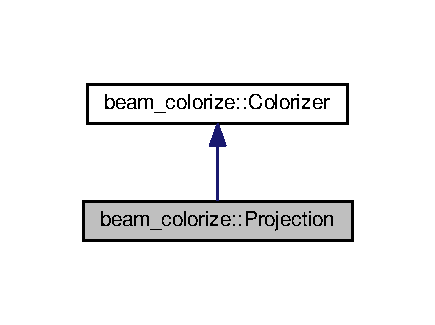
\includegraphics[width=209pt]{classbeam__colorize_1_1_projection__inherit__graph}
\end{center}
\end{figure}


Collaboration diagram for beam\+\_\+colorize\+:\+:Projection\+:\nopagebreak
\begin{figure}[H]
\begin{center}
\leavevmode
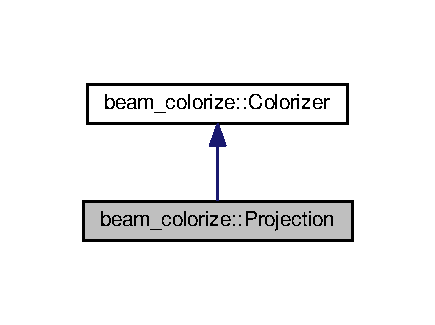
\includegraphics[width=209pt]{classbeam__colorize_1_1_projection__coll__graph}
\end{center}
\end{figure}
\subsection*{Public Member Functions}
\begin{DoxyCompactItemize}
\item 
\hyperlink{classbeam__colorize_1_1_projection_a7f1eea1ad6db0d40278b79c622d09b9b}{Projection} ()=default
\item 
\hyperlink{classbeam__colorize_1_1_projection_a5bc4fa859a4c029f429f0250ac8711f8}{$\sim$\+Projection} () override=default
\item 
pcl\+::\+Point\+Cloud$<$ pcl\+::\+Point\+X\+Y\+Z\+R\+GB $>$\+::Ptr \hyperlink{classbeam__colorize_1_1_projection_a23a0d92d022d6a65647b4d15a462c35a}{Colorize\+Point\+Cloud} (const pcl\+::\+Point\+Cloud$<$ pcl\+::\+Point\+X\+YZ $>$ \&input\+\_\+cloud, const sensor\+\_\+msgs\+::\+Image \&input\+\_\+image) const override
\begin{DoxyCompactList}\small\item\em Method for colorizing a point cloud from an image. \end{DoxyCompactList}\end{DoxyCompactItemize}


\subsection{Detailed Description}
Class which implements \hyperlink{classbeam__colorize_1_1_colorizer}{Colorizer} interface and provides colorization functionality using projection methods. 

Definition at line 16 of file Projection.\+h.



\subsection{Constructor \& Destructor Documentation}
\index{beam\+\_\+colorize\+::\+Projection@{beam\+\_\+colorize\+::\+Projection}!Projection@{Projection}}
\index{Projection@{Projection}!beam\+\_\+colorize\+::\+Projection@{beam\+\_\+colorize\+::\+Projection}}
\subsubsection[{\texorpdfstring{Projection()=default}{Projection()=default}}]{\setlength{\rightskip}{0pt plus 5cm}beam\+\_\+colorize\+::\+Projection\+::\+Projection (
\begin{DoxyParamCaption}
{}
\end{DoxyParamCaption}
)\hspace{0.3cm}{\ttfamily [default]}}\hypertarget{classbeam__colorize_1_1_projection_a7f1eea1ad6db0d40278b79c622d09b9b}{}\label{classbeam__colorize_1_1_projection_a7f1eea1ad6db0d40278b79c622d09b9b}
\index{beam\+\_\+colorize\+::\+Projection@{beam\+\_\+colorize\+::\+Projection}!````~Projection@{$\sim$\+Projection}}
\index{````~Projection@{$\sim$\+Projection}!beam\+\_\+colorize\+::\+Projection@{beam\+\_\+colorize\+::\+Projection}}
\subsubsection[{\texorpdfstring{$\sim$\+Projection() override=default}{~Projection() override=default}}]{\setlength{\rightskip}{0pt plus 5cm}beam\+\_\+colorize\+::\+Projection\+::$\sim$\+Projection (
\begin{DoxyParamCaption}
{}
\end{DoxyParamCaption}
)\hspace{0.3cm}{\ttfamily [override]}, {\ttfamily [default]}}\hypertarget{classbeam__colorize_1_1_projection_a5bc4fa859a4c029f429f0250ac8711f8}{}\label{classbeam__colorize_1_1_projection_a5bc4fa859a4c029f429f0250ac8711f8}


\subsection{Member Function Documentation}
\index{beam\+\_\+colorize\+::\+Projection@{beam\+\_\+colorize\+::\+Projection}!Colorize\+Point\+Cloud@{Colorize\+Point\+Cloud}}
\index{Colorize\+Point\+Cloud@{Colorize\+Point\+Cloud}!beam\+\_\+colorize\+::\+Projection@{beam\+\_\+colorize\+::\+Projection}}
\subsubsection[{\texorpdfstring{Colorize\+Point\+Cloud(const pcl\+::\+Point\+Cloud$<$ pcl\+::\+Point\+X\+Y\+Z $>$ \&input\+\_\+cloud, const sensor\+\_\+msgs\+::\+Image \&input\+\_\+image) const override}{ColorizePointCloud(const pcl::PointCloud< pcl::PointXYZ > &input_cloud, const sensor_msgs::Image &input_image) const override}}]{\setlength{\rightskip}{0pt plus 5cm}pcl\+::\+Point\+Cloud$<$ pcl\+::\+Point\+X\+Y\+Z\+R\+GB $>$\+::Ptr beam\+\_\+colorize\+::\+Projection\+::\+Colorize\+Point\+Cloud (
\begin{DoxyParamCaption}
\item[{const pcl\+::\+Point\+Cloud$<$ pcl\+::\+Point\+X\+YZ $>$ \&}]{input\+\_\+cloud, }
\item[{const sensor\+\_\+msgs\+::\+Image \&}]{input\+\_\+image}
\end{DoxyParamCaption}
) const\hspace{0.3cm}{\ttfamily [override]}, {\ttfamily [virtual]}}\hypertarget{classbeam__colorize_1_1_projection_a23a0d92d022d6a65647b4d15a462c35a}{}\label{classbeam__colorize_1_1_projection_a23a0d92d022d6a65647b4d15a462c35a}


Method for colorizing a point cloud from an image. 


\begin{DoxyParams}{Parameters}
{\em input\+\_\+cloud} & Input point cloud in the camera frame \\
\hline
{\em input\+\_\+image} & Image which will be used to color point cloud \\
\hline
\end{DoxyParams}
\begin{DoxyReturn}{Returns}
Colored point cloud 
\end{DoxyReturn}


Implements \hyperlink{classbeam__colorize_1_1_colorizer_ab9ca2ddf55fd8782e6b31c64e85efcbc}{beam\+\_\+colorize\+::\+Colorizer}.



Definition at line 30 of file Projection.\+cpp.



The documentation for this class was generated from the following files\+:\begin{DoxyCompactItemize}
\item 
beam\+\_\+colorize/include/beam/colorize/\hyperlink{_projection_8h}{Projection.\+h}\item 
beam\+\_\+colorize/src/\hyperlink{_projection_8cpp}{Projection.\+cpp}\end{DoxyCompactItemize}

\hypertarget{classbeam__colorize_1_1_ray_trace}{}\section{beam\+\_\+colorize\+:\+:Ray\+Trace Class Reference}
\label{classbeam__colorize_1_1_ray_trace}\index{beam\+\_\+colorize\+::\+Ray\+Trace@{beam\+\_\+colorize\+::\+Ray\+Trace}}


Class which implements \hyperlink{classbeam__colorize_1_1_colorizer}{Colorizer} interface and provides colorization functionality using ray tracing.  




{\ttfamily \#include $<$Ray\+Trace.\+h$>$}



Inheritance diagram for beam\+\_\+colorize\+:\+:Ray\+Trace\+:\nopagebreak
\begin{figure}[H]
\begin{center}
\leavevmode
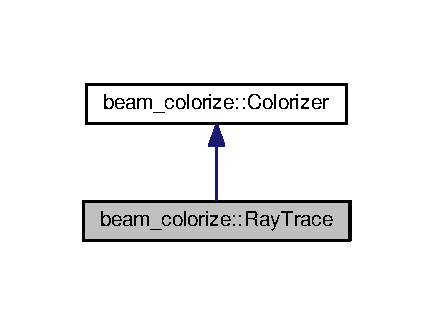
\includegraphics[width=208pt]{classbeam__colorize_1_1_ray_trace__inherit__graph}
\end{center}
\end{figure}


Collaboration diagram for beam\+\_\+colorize\+:\+:Ray\+Trace\+:\nopagebreak
\begin{figure}[H]
\begin{center}
\leavevmode
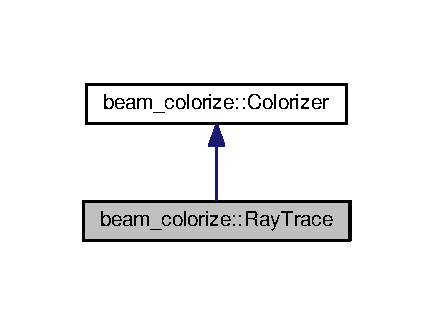
\includegraphics[width=208pt]{classbeam__colorize_1_1_ray_trace__coll__graph}
\end{center}
\end{figure}
\subsection*{Public Member Functions}
\begin{DoxyCompactItemize}
\item 
\hyperlink{classbeam__colorize_1_1_ray_trace_aec8057d228e016bb430f62bde570ef0e}{Ray\+Trace} ()=default
\item 
\hyperlink{classbeam__colorize_1_1_ray_trace_a485d3ab719933747688e248835db1abb}{$\sim$\+Ray\+Trace} ()=default
\item 
pcl\+::\+Point\+Cloud$<$ pcl\+::\+Point\+X\+Y\+Z\+R\+GB $>$\+::Ptr \hyperlink{classbeam__colorize_1_1_ray_trace_a41c414265166ecb12e32d976120ce157}{Colorize\+Point\+Cloud} (const pcl\+::\+Point\+Cloud$<$ pcl\+::\+Point\+X\+YZ $>$ \&input\+\_\+cloud, const sensor\+\_\+msgs\+::\+Image \&input\+\_\+image) const override
\begin{DoxyCompactList}\small\item\em Method for colorizing a point cloud from an image. \end{DoxyCompactList}\end{DoxyCompactItemize}


\subsection{Detailed Description}
Class which implements \hyperlink{classbeam__colorize_1_1_colorizer}{Colorizer} interface and provides colorization functionality using ray tracing. 

Definition at line 17 of file Ray\+Trace.\+h.



\subsection{Constructor \& Destructor Documentation}
\index{beam\+\_\+colorize\+::\+Ray\+Trace@{beam\+\_\+colorize\+::\+Ray\+Trace}!Ray\+Trace@{Ray\+Trace}}
\index{Ray\+Trace@{Ray\+Trace}!beam\+\_\+colorize\+::\+Ray\+Trace@{beam\+\_\+colorize\+::\+Ray\+Trace}}
\subsubsection[{\texorpdfstring{Ray\+Trace()=default}{RayTrace()=default}}]{\setlength{\rightskip}{0pt plus 5cm}beam\+\_\+colorize\+::\+Ray\+Trace\+::\+Ray\+Trace (
\begin{DoxyParamCaption}
{}
\end{DoxyParamCaption}
)\hspace{0.3cm}{\ttfamily [default]}}\hypertarget{classbeam__colorize_1_1_ray_trace_aec8057d228e016bb430f62bde570ef0e}{}\label{classbeam__colorize_1_1_ray_trace_aec8057d228e016bb430f62bde570ef0e}
\index{beam\+\_\+colorize\+::\+Ray\+Trace@{beam\+\_\+colorize\+::\+Ray\+Trace}!````~Ray\+Trace@{$\sim$\+Ray\+Trace}}
\index{````~Ray\+Trace@{$\sim$\+Ray\+Trace}!beam\+\_\+colorize\+::\+Ray\+Trace@{beam\+\_\+colorize\+::\+Ray\+Trace}}
\subsubsection[{\texorpdfstring{$\sim$\+Ray\+Trace()=default}{~RayTrace()=default}}]{\setlength{\rightskip}{0pt plus 5cm}beam\+\_\+colorize\+::\+Ray\+Trace\+::$\sim$\+Ray\+Trace (
\begin{DoxyParamCaption}
{}
\end{DoxyParamCaption}
)\hspace{0.3cm}{\ttfamily [default]}}\hypertarget{classbeam__colorize_1_1_ray_trace_a485d3ab719933747688e248835db1abb}{}\label{classbeam__colorize_1_1_ray_trace_a485d3ab719933747688e248835db1abb}


\subsection{Member Function Documentation}
\index{beam\+\_\+colorize\+::\+Ray\+Trace@{beam\+\_\+colorize\+::\+Ray\+Trace}!Colorize\+Point\+Cloud@{Colorize\+Point\+Cloud}}
\index{Colorize\+Point\+Cloud@{Colorize\+Point\+Cloud}!beam\+\_\+colorize\+::\+Ray\+Trace@{beam\+\_\+colorize\+::\+Ray\+Trace}}
\subsubsection[{\texorpdfstring{Colorize\+Point\+Cloud(const pcl\+::\+Point\+Cloud$<$ pcl\+::\+Point\+X\+Y\+Z $>$ \&input\+\_\+cloud, const sensor\+\_\+msgs\+::\+Image \&input\+\_\+image) const override}{ColorizePointCloud(const pcl::PointCloud< pcl::PointXYZ > &input_cloud, const sensor_msgs::Image &input_image) const override}}]{\setlength{\rightskip}{0pt plus 5cm}pcl\+::\+Point\+Cloud$<$ pcl\+::\+Point\+X\+Y\+Z\+R\+GB $>$\+::Ptr beam\+\_\+colorize\+::\+Ray\+Trace\+::\+Colorize\+Point\+Cloud (
\begin{DoxyParamCaption}
\item[{const pcl\+::\+Point\+Cloud$<$ pcl\+::\+Point\+X\+YZ $>$ \&}]{input\+\_\+cloud, }
\item[{const sensor\+\_\+msgs\+::\+Image \&}]{input\+\_\+image}
\end{DoxyParamCaption}
) const\hspace{0.3cm}{\ttfamily [override]}, {\ttfamily [virtual]}}\hypertarget{classbeam__colorize_1_1_ray_trace_a41c414265166ecb12e32d976120ce157}{}\label{classbeam__colorize_1_1_ray_trace_a41c414265166ecb12e32d976120ce157}


Method for colorizing a point cloud from an image. 


\begin{DoxyParams}{Parameters}
{\em input\+\_\+cloud} & Input point cloud in the camera frame \\
\hline
{\em input\+\_\+image} & Image which will be used to color point cloud \\
\hline
\end{DoxyParams}
\begin{DoxyReturn}{Returns}
Colored point cloud 
\end{DoxyReturn}


Implements \hyperlink{classbeam__colorize_1_1_colorizer_ab9ca2ddf55fd8782e6b31c64e85efcbc}{beam\+\_\+colorize\+::\+Colorizer}.



Definition at line 5 of file Ray\+Trace.\+cpp.



The documentation for this class was generated from the following files\+:\begin{DoxyCompactItemize}
\item 
beam\+\_\+colorize/include/beam/colorize/\hyperlink{_ray_trace_8h}{Ray\+Trace.\+h}\item 
beam\+\_\+colorize/src/\hyperlink{_ray_trace_8cpp}{Ray\+Trace.\+cpp}\end{DoxyCompactItemize}

\hypertarget{classbeam__defects_1_1_spall}{}\section{beam\+\_\+defects\+:\+:Spall Class Reference}
\label{classbeam__defects_1_1_spall}\index{beam\+\_\+defects\+::\+Spall@{beam\+\_\+defects\+::\+Spall}}


Derived class for spall defects.  




{\ttfamily \#include $<$Spall.\+h$>$}



Inheritance diagram for beam\+\_\+defects\+:\+:Spall\+:\nopagebreak
\begin{figure}[H]
\begin{center}
\leavevmode
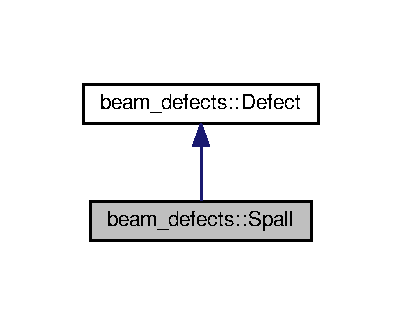
\includegraphics[width=193pt]{classbeam__defects_1_1_spall__inherit__graph}
\end{center}
\end{figure}


Collaboration diagram for beam\+\_\+defects\+:\+:Spall\+:\nopagebreak
\begin{figure}[H]
\begin{center}
\leavevmode
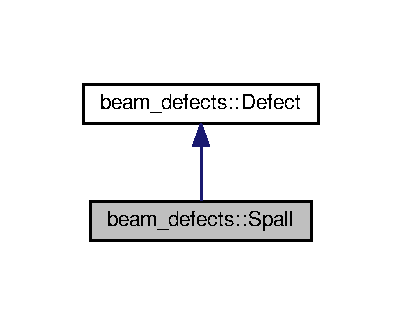
\includegraphics[width=193pt]{classbeam__defects_1_1_spall__coll__graph}
\end{center}
\end{figure}
\subsection*{Public Member Functions}
\begin{DoxyCompactItemize}
\item 
\hyperlink{classbeam__defects_1_1_spall_a6b4a13b64813a69284779151178459fb}{Spall} ()=default
\begin{DoxyCompactList}\small\item\em Default constructor. \end{DoxyCompactList}\item 
\hyperlink{classbeam__defects_1_1_spall_a19277f2779003d9379892c6fff087c16}{Spall} (pcl\+::\+Point\+Cloud$<$ pcl\+::\+Point\+X\+YZ $>$\+::\hyperlink{classbeam__defects_1_1_defect_a0a7708c6cd92ac482d45ef606d598325}{Ptr} pc)
\begin{DoxyCompactList}\small\item\em Construct with a point cloud. \end{DoxyCompactList}\item 
\hyperlink{classbeam__defects_1_1_spall_a0af44141e40c87c68ef20e7194476680}{$\sim$\+Spall} () override=default
\begin{DoxyCompactList}\small\item\em Default constructor. \end{DoxyCompactList}\item 
\hyperlink{group__defects_gae379b271bd5fb7ce92afe1abee917249}{Defect\+Type} \hyperlink{classbeam__defects_1_1_spall_a98572b81bfd78594f1e497758946aaa1}{Get\+Type} () const override
\begin{DoxyCompactList}\small\item\em Get the type of defect. \end{DoxyCompactList}\item 
double \hyperlink{classbeam__defects_1_1_spall_a84f5aaa8ced3ae1c61eb8f77e540c466}{Get\+Size} () override
\begin{DoxyCompactList}\small\item\em Get the size of the defect. \end{DoxyCompactList}\item 
\hyperlink{group__defects_gaed38c449f8cba57f35d1af04496a0711}{Defect\+O\+S\+I\+M\+Severity} \hyperlink{classbeam__defects_1_1_spall_a96f74134abee749d37cf750119098c4c}{Get\+O\+S\+I\+M\+Severity} () override
\end{DoxyCompactItemize}
\subsection*{Additional Inherited Members}


\subsection{Detailed Description}
Derived class for spall defects. 

Definition at line 15 of file Spall.\+h.



\subsection{Constructor \& Destructor Documentation}
\index{beam\+\_\+defects\+::\+Spall@{beam\+\_\+defects\+::\+Spall}!Spall@{Spall}}
\index{Spall@{Spall}!beam\+\_\+defects\+::\+Spall@{beam\+\_\+defects\+::\+Spall}}
\subsubsection[{\texorpdfstring{Spall()=default}{Spall()=default}}]{\setlength{\rightskip}{0pt plus 5cm}beam\+\_\+defects\+::\+Spall\+::\+Spall (
\begin{DoxyParamCaption}
{}
\end{DoxyParamCaption}
)\hspace{0.3cm}{\ttfamily [default]}}\hypertarget{classbeam__defects_1_1_spall_a6b4a13b64813a69284779151178459fb}{}\label{classbeam__defects_1_1_spall_a6b4a13b64813a69284779151178459fb}


Default constructor. 

\index{beam\+\_\+defects\+::\+Spall@{beam\+\_\+defects\+::\+Spall}!Spall@{Spall}}
\index{Spall@{Spall}!beam\+\_\+defects\+::\+Spall@{beam\+\_\+defects\+::\+Spall}}
\subsubsection[{\texorpdfstring{Spall(pcl\+::\+Point\+Cloud$<$ pcl\+::\+Point\+X\+Y\+Z $>$\+::\+Ptr pc)}{Spall(pcl::PointCloud< pcl::PointXYZ >::Ptr pc)}}]{\setlength{\rightskip}{0pt plus 5cm}beam\+\_\+defects\+::\+Spall\+::\+Spall (
\begin{DoxyParamCaption}
\item[{pcl\+::\+Point\+Cloud$<$ pcl\+::\+Point\+X\+YZ $>$\+::{\bf Ptr}}]{pc}
\end{DoxyParamCaption}
)\hspace{0.3cm}{\ttfamily [explicit]}}\hypertarget{classbeam__defects_1_1_spall_a19277f2779003d9379892c6fff087c16}{}\label{classbeam__defects_1_1_spall_a19277f2779003d9379892c6fff087c16}


Construct with a point cloud. 


\begin{DoxyParams}{Parameters}
{\em pc} & \\
\hline
\end{DoxyParams}


Definition at line 6 of file Spall.\+cpp.

\index{beam\+\_\+defects\+::\+Spall@{beam\+\_\+defects\+::\+Spall}!````~Spall@{$\sim$\+Spall}}
\index{````~Spall@{$\sim$\+Spall}!beam\+\_\+defects\+::\+Spall@{beam\+\_\+defects\+::\+Spall}}
\subsubsection[{\texorpdfstring{$\sim$\+Spall() override=default}{~Spall() override=default}}]{\setlength{\rightskip}{0pt plus 5cm}beam\+\_\+defects\+::\+Spall\+::$\sim$\+Spall (
\begin{DoxyParamCaption}
{}
\end{DoxyParamCaption}
)\hspace{0.3cm}{\ttfamily [override]}, {\ttfamily [default]}}\hypertarget{classbeam__defects_1_1_spall_a0af44141e40c87c68ef20e7194476680}{}\label{classbeam__defects_1_1_spall_a0af44141e40c87c68ef20e7194476680}


Default constructor. 



\subsection{Member Function Documentation}
\index{beam\+\_\+defects\+::\+Spall@{beam\+\_\+defects\+::\+Spall}!Get\+O\+S\+I\+M\+Severity@{Get\+O\+S\+I\+M\+Severity}}
\index{Get\+O\+S\+I\+M\+Severity@{Get\+O\+S\+I\+M\+Severity}!beam\+\_\+defects\+::\+Spall@{beam\+\_\+defects\+::\+Spall}}
\subsubsection[{\texorpdfstring{Get\+O\+S\+I\+M\+Severity() override}{GetOSIMSeverity() override}}]{\setlength{\rightskip}{0pt plus 5cm}{\bf Defect\+O\+S\+I\+M\+Severity} beam\+\_\+defects\+::\+Spall\+::\+Get\+O\+S\+I\+M\+Severity (
\begin{DoxyParamCaption}
{}
\end{DoxyParamCaption}
)\hspace{0.3cm}{\ttfamily [override]}, {\ttfamily [virtual]}}\hypertarget{classbeam__defects_1_1_spall_a96f74134abee749d37cf750119098c4c}{}\label{classbeam__defects_1_1_spall_a96f74134abee749d37cf750119098c4c}


Implements \hyperlink{classbeam__defects_1_1_defect_a74824cc5cdb9d301d72089585ed8f1f2}{beam\+\_\+defects\+::\+Defect}.



Definition at line 28 of file Spall.\+cpp.

\index{beam\+\_\+defects\+::\+Spall@{beam\+\_\+defects\+::\+Spall}!Get\+Size@{Get\+Size}}
\index{Get\+Size@{Get\+Size}!beam\+\_\+defects\+::\+Spall@{beam\+\_\+defects\+::\+Spall}}
\subsubsection[{\texorpdfstring{Get\+Size() override}{GetSize() override}}]{\setlength{\rightskip}{0pt plus 5cm}double beam\+\_\+defects\+::\+Spall\+::\+Get\+Size (
\begin{DoxyParamCaption}
{}
\end{DoxyParamCaption}
)\hspace{0.3cm}{\ttfamily [override]}, {\ttfamily [virtual]}}\hypertarget{classbeam__defects_1_1_spall_a84f5aaa8ced3ae1c61eb8f77e540c466}{}\label{classbeam__defects_1_1_spall_a84f5aaa8ced3ae1c61eb8f77e540c466}


Get the size of the defect. 

\begin{DoxyReturn}{Returns}
Returns the size of the defect in whatever units are relevant for this class of defect 
\end{DoxyReturn}


Implements \hyperlink{classbeam__defects_1_1_defect_aa7c24d68d22e6d47dc1b9e8a9ad94c56}{beam\+\_\+defects\+::\+Defect}.



Definition at line 8 of file Spall.\+cpp.

\index{beam\+\_\+defects\+::\+Spall@{beam\+\_\+defects\+::\+Spall}!Get\+Type@{Get\+Type}}
\index{Get\+Type@{Get\+Type}!beam\+\_\+defects\+::\+Spall@{beam\+\_\+defects\+::\+Spall}}
\subsubsection[{\texorpdfstring{Get\+Type() const override}{GetType() const override}}]{\setlength{\rightskip}{0pt plus 5cm}{\bf Defect\+Type} beam\+\_\+defects\+::\+Spall\+::\+Get\+Type (
\begin{DoxyParamCaption}
{}
\end{DoxyParamCaption}
) const\hspace{0.3cm}{\ttfamily [inline]}, {\ttfamily [override]}, {\ttfamily [virtual]}}\hypertarget{classbeam__defects_1_1_spall_a98572b81bfd78594f1e497758946aaa1}{}\label{classbeam__defects_1_1_spall_a98572b81bfd78594f1e497758946aaa1}


Get the type of defect. 

\begin{DoxyReturn}{Returns}
Returns type as one of defects specified in the enum Defect\+Type 
\end{DoxyReturn}


Implements \hyperlink{classbeam__defects_1_1_defect_aab237fd856c7ace882ead216c81574e6}{beam\+\_\+defects\+::\+Defect}.



Definition at line 37 of file Spall.\+h.



The documentation for this class was generated from the following files\+:\begin{DoxyCompactItemize}
\item 
beam\+\_\+defects/include/beam\+\_\+defects/\hyperlink{_spall_8h}{Spall.\+h}\item 
beam\+\_\+defects/src/\hyperlink{_spall_8cpp}{Spall.\+cpp}\end{DoxyCompactItemize}

\hypertarget{classbeam__calibration_1_1_tf_tree}{}\section{beam\+\_\+calibration\+:\+:Tf\+Tree Class Reference}
\label{classbeam__calibration_1_1_tf_tree}\index{beam\+\_\+calibration\+::\+Tf\+Tree@{beam\+\_\+calibration\+::\+Tf\+Tree}}


Class for managing extrinsic transformation tree using the tf2 library.  




{\ttfamily \#include $<$Tf\+Tree.\+h$>$}

\subsection*{Public Member Functions}
\begin{DoxyCompactItemize}
\item 
\hyperlink{classbeam__calibration_1_1_tf_tree_aec864eabffcbeb3c0e914d3a90b2e671}{Tf\+Tree} ()=default
\begin{DoxyCompactList}\small\item\em Default constructor. \end{DoxyCompactList}\item 
\hyperlink{classbeam__calibration_1_1_tf_tree_a99292e90192a114388933b1d04346151}{$\sim$\+Tf\+Tree} ()=default
\begin{DoxyCompactList}\small\item\em Default constructor. \end{DoxyCompactList}\item 
void \hyperlink{classbeam__calibration_1_1_tf_tree_a25115497d8169ffec43a204770ca3436}{Add\+Transform} (Eigen\+::\+Affine3d \&Tnew, std\+::string \&to\+\_\+frame, std\+::string \&from\+\_\+frame, std\+::string \&calib\+\_\+date)
\begin{DoxyCompactList}\small\item\em Method for adding a transformation using an Affine3d. \end{DoxyCompactList}\item 
Eigen\+::\+Affine3d \hyperlink{classbeam__calibration_1_1_tf_tree_a4cc7847b4fa5a728327759446df7f14c}{Get\+Transform} (std\+::string \&to\+\_\+frame, std\+::string \&from\+\_\+frame)
\begin{DoxyCompactList}\small\item\em Method for retrieving a transformation. \end{DoxyCompactList}\item 
std\+::string \hyperlink{classbeam__calibration_1_1_tf_tree_aa8ea53149a8bc97ebf11d86448db17d5}{Get\+Calibration\+Date} ()
\begin{DoxyCompactList}\small\item\em Method for retrieving the date that the calibration was done. \end{DoxyCompactList}\end{DoxyCompactItemize}


\subsection{Detailed Description}
Class for managing extrinsic transformation tree using the tf2 library. 

Definition at line 21 of file Tf\+Tree.\+h.



\subsection{Constructor \& Destructor Documentation}
\index{beam\+\_\+calibration\+::\+Tf\+Tree@{beam\+\_\+calibration\+::\+Tf\+Tree}!Tf\+Tree@{Tf\+Tree}}
\index{Tf\+Tree@{Tf\+Tree}!beam\+\_\+calibration\+::\+Tf\+Tree@{beam\+\_\+calibration\+::\+Tf\+Tree}}
\subsubsection[{\texorpdfstring{Tf\+Tree()=default}{TfTree()=default}}]{\setlength{\rightskip}{0pt plus 5cm}beam\+\_\+calibration\+::\+Tf\+Tree\+::\+Tf\+Tree (
\begin{DoxyParamCaption}
{}
\end{DoxyParamCaption}
)\hspace{0.3cm}{\ttfamily [default]}}\hypertarget{classbeam__calibration_1_1_tf_tree_aec864eabffcbeb3c0e914d3a90b2e671}{}\label{classbeam__calibration_1_1_tf_tree_aec864eabffcbeb3c0e914d3a90b2e671}


Default constructor. 

\index{beam\+\_\+calibration\+::\+Tf\+Tree@{beam\+\_\+calibration\+::\+Tf\+Tree}!````~Tf\+Tree@{$\sim$\+Tf\+Tree}}
\index{````~Tf\+Tree@{$\sim$\+Tf\+Tree}!beam\+\_\+calibration\+::\+Tf\+Tree@{beam\+\_\+calibration\+::\+Tf\+Tree}}
\subsubsection[{\texorpdfstring{$\sim$\+Tf\+Tree()=default}{~TfTree()=default}}]{\setlength{\rightskip}{0pt plus 5cm}beam\+\_\+calibration\+::\+Tf\+Tree\+::$\sim$\+Tf\+Tree (
\begin{DoxyParamCaption}
{}
\end{DoxyParamCaption}
)\hspace{0.3cm}{\ttfamily [default]}}\hypertarget{classbeam__calibration_1_1_tf_tree_a99292e90192a114388933b1d04346151}{}\label{classbeam__calibration_1_1_tf_tree_a99292e90192a114388933b1d04346151}


Default constructor. 



\subsection{Member Function Documentation}
\index{beam\+\_\+calibration\+::\+Tf\+Tree@{beam\+\_\+calibration\+::\+Tf\+Tree}!Add\+Transform@{Add\+Transform}}
\index{Add\+Transform@{Add\+Transform}!beam\+\_\+calibration\+::\+Tf\+Tree@{beam\+\_\+calibration\+::\+Tf\+Tree}}
\subsubsection[{\texorpdfstring{Add\+Transform(\+Eigen\+::\+Affine3d \&\+Tnew, std\+::string \&to\+\_\+frame, std\+::string \&from\+\_\+frame, std\+::string \&calib\+\_\+date)}{AddTransform(Eigen::Affine3d &Tnew, std::string &to_frame, std::string &from_frame, std::string &calib_date)}}]{\setlength{\rightskip}{0pt plus 5cm}void beam\+\_\+calibration\+::\+Tf\+Tree\+::\+Add\+Transform (
\begin{DoxyParamCaption}
\item[{Eigen\+::\+Affine3d \&}]{Tnew, }
\item[{std\+::string \&}]{to\+\_\+frame, }
\item[{std\+::string \&}]{from\+\_\+frame, }
\item[{std\+::string \&}]{calib\+\_\+date}
\end{DoxyParamCaption}
)}\hypertarget{classbeam__calibration_1_1_tf_tree_a25115497d8169ffec43a204770ca3436}{}\label{classbeam__calibration_1_1_tf_tree_a25115497d8169ffec43a204770ca3436}


Method for adding a transformation using an Affine3d. 



Definition at line 9 of file Tf\+Tree.\+cpp.

\index{beam\+\_\+calibration\+::\+Tf\+Tree@{beam\+\_\+calibration\+::\+Tf\+Tree}!Get\+Calibration\+Date@{Get\+Calibration\+Date}}
\index{Get\+Calibration\+Date@{Get\+Calibration\+Date}!beam\+\_\+calibration\+::\+Tf\+Tree@{beam\+\_\+calibration\+::\+Tf\+Tree}}
\subsubsection[{\texorpdfstring{Get\+Calibration\+Date()}{GetCalibrationDate()}}]{\setlength{\rightskip}{0pt plus 5cm}std\+::string beam\+\_\+calibration\+::\+Tf\+Tree\+::\+Get\+Calibration\+Date (
\begin{DoxyParamCaption}
{}
\end{DoxyParamCaption}
)}\hypertarget{classbeam__calibration_1_1_tf_tree_aa8ea53149a8bc97ebf11d86448db17d5}{}\label{classbeam__calibration_1_1_tf_tree_aa8ea53149a8bc97ebf11d86448db17d5}


Method for retrieving the date that the calibration was done. 

\begin{DoxyReturn}{Returns}
Return calibration date 
\end{DoxyReturn}


Definition at line 48 of file Tf\+Tree.\+cpp.

\index{beam\+\_\+calibration\+::\+Tf\+Tree@{beam\+\_\+calibration\+::\+Tf\+Tree}!Get\+Transform@{Get\+Transform}}
\index{Get\+Transform@{Get\+Transform}!beam\+\_\+calibration\+::\+Tf\+Tree@{beam\+\_\+calibration\+::\+Tf\+Tree}}
\subsubsection[{\texorpdfstring{Get\+Transform(std\+::string \&to\+\_\+frame, std\+::string \&from\+\_\+frame)}{GetTransform(std::string &to_frame, std::string &from_frame)}}]{\setlength{\rightskip}{0pt plus 5cm}Eigen\+::\+Affine3d beam\+\_\+calibration\+::\+Tf\+Tree\+::\+Get\+Transform (
\begin{DoxyParamCaption}
\item[{std\+::string \&}]{to\+\_\+frame, }
\item[{std\+::string \&}]{from\+\_\+frame}
\end{DoxyParamCaption}
)}\hypertarget{classbeam__calibration_1_1_tf_tree_a4cc7847b4fa5a728327759446df7f14c}{}\label{classbeam__calibration_1_1_tf_tree_a4cc7847b4fa5a728327759446df7f14c}


Method for retrieving a transformation. 

\begin{DoxyReturn}{Returns}
Return the transformation requested as Affine3d object 
\end{DoxyReturn}


Definition at line 25 of file Tf\+Tree.\+cpp.



The documentation for this class was generated from the following files\+:\begin{DoxyCompactItemize}
\item 
beam\+\_\+calibration/include/beam/calibration/\hyperlink{_tf_tree_8h}{Tf\+Tree.\+h}\item 
beam\+\_\+calibration/src/\hyperlink{_tf_tree_8cpp}{Tf\+Tree.\+cpp}\end{DoxyCompactItemize}

\hypertarget{structbeam_1_1_vec_comparator}{}\section{beam\+:\+:Vec\+Comparator Struct Reference}
\label{structbeam_1_1_vec_comparator}\index{beam\+::\+Vec\+Comparator@{beam\+::\+Vec\+Comparator}}


{\ttfamily \#include $<$math.\+hpp$>$}

\subsection*{Public Member Functions}
\begin{DoxyCompactItemize}
\item 
bool \hyperlink{structbeam_1_1_vec_comparator_a2e9749f17079f6b499b11f4ee66eb159}{operator()} (const \hyperlink{group__utils_gae5ba967e4b0d4b421ca30ef46f896145}{VecX} \&a, const \hyperlink{group__utils_gae5ba967e4b0d4b421ca30ef46f896145}{VecX} \&b) const 
\end{DoxyCompactItemize}


\subsection{Detailed Description}
Eigen vector comparator 

Definition at line 48 of file math.\+hpp.



\subsection{Member Function Documentation}
\index{beam\+::\+Vec\+Comparator@{beam\+::\+Vec\+Comparator}!operator()@{operator()}}
\index{operator()@{operator()}!beam\+::\+Vec\+Comparator@{beam\+::\+Vec\+Comparator}}
\subsubsection[{\texorpdfstring{operator()(const Vec\+X \&a, const Vec\+X \&b) const }{operator()(const VecX &a, const VecX &b) const }}]{\setlength{\rightskip}{0pt plus 5cm}bool beam\+::\+Vec\+Comparator\+::operator() (
\begin{DoxyParamCaption}
\item[{const {\bf VecX} \&}]{a, }
\item[{const {\bf VecX} \&}]{b}
\end{DoxyParamCaption}
) const\hspace{0.3cm}{\ttfamily [inline]}}\hypertarget{structbeam_1_1_vec_comparator_a2e9749f17079f6b499b11f4ee66eb159}{}\label{structbeam_1_1_vec_comparator_a2e9749f17079f6b499b11f4ee66eb159}


Definition at line 49 of file math.\+hpp.



The documentation for this struct was generated from the following file\+:\begin{DoxyCompactItemize}
\item 
beam\+\_\+utils/include/beam/utils/\hyperlink{math_8hpp}{math.\+hpp}\end{DoxyCompactItemize}

\chapter{File Documentation}
\hypertarget{_fisheye_8h}{}\section{beam\+\_\+calibration/include/beam/calibration/\+Fisheye.h File Reference}
\label{_fisheye_8h}\index{beam\+\_\+calibration/include/beam/calibration/\+Fisheye.\+h@{beam\+\_\+calibration/include/beam/calibration/\+Fisheye.\+h}}

\hypertarget{_intrinsics_8h}{}\section{beam\+\_\+calibration/include/beam/calibration/\+Intrinsics.h File Reference}
\label{_intrinsics_8h}\index{beam\+\_\+calibration/include/beam/calibration/\+Intrinsics.\+h@{beam\+\_\+calibration/include/beam/calibration/\+Intrinsics.\+h}}
{\ttfamily \#include \char`\"{}beam/utils/math.\+hpp\char`\"{}}\\*
Include dependency graph for Intrinsics.\+h\+:\nopagebreak
\begin{figure}[H]
\begin{center}
\leavevmode
\includegraphics[width=350pt]{_intrinsics_8h__incl}
\end{center}
\end{figure}
This graph shows which files directly or indirectly include this file\+:\nopagebreak
\begin{figure}[H]
\begin{center}
\leavevmode
\includegraphics[width=350pt]{_intrinsics_8h__dep__incl}
\end{center}
\end{figure}
\subsection*{Classes}
\begin{DoxyCompactItemize}
\item 
class \hyperlink{classbeam__calibration_1_1_intrinsics}{beam\+\_\+calibration\+::\+Intrinsics}
\begin{DoxyCompactList}\small\item\em Abstract class for calibrations. \end{DoxyCompactList}\end{DoxyCompactItemize}
\subsection*{Namespaces}
\begin{DoxyCompactItemize}
\item 
 \hyperlink{namespacebeam__calibration}{beam\+\_\+calibration}
\end{DoxyCompactItemize}
\subsection*{Enumerations}
\begin{DoxyCompactItemize}
\item 
enum \hyperlink{group__calibration_ga9abafc7bdd7c31c8fdbd4cc90df9a956}{beam\+\_\+calibration\+::\+Intrinsics\+Type} \{ \hyperlink{group__calibration_gga9abafc7bdd7c31c8fdbd4cc90df9a956aa26b5d5659fbc90615fd36cf5d0a29c0}{beam\+\_\+calibration\+::\+Intrinsics\+Type\+::\+P\+I\+N\+H\+O\+LE} = 0, 
\hyperlink{group__calibration_gga9abafc7bdd7c31c8fdbd4cc90df9a956a59fe84c43d228f3307801ba9f7151157}{beam\+\_\+calibration\+::\+Intrinsics\+Type\+::\+F\+I\+S\+H\+E\+YE}, 
\hyperlink{group__calibration_gga9abafc7bdd7c31c8fdbd4cc90df9a956ad58295f6b3fb30f0c66af9f7f8a7cfd9}{beam\+\_\+calibration\+::\+Intrinsics\+Type\+::\+L\+A\+D\+Y\+B\+UG}
 \}\begin{DoxyCompactList}\small\item\em Enum class for different types of intrinsic calibrations. \end{DoxyCompactList}
\end{DoxyCompactItemize}

\hypertarget{_ladybug_8h}{}\section{beam\+\_\+calibration/include/beam/calibration/\+Ladybug.h File Reference}
\label{_ladybug_8h}\index{beam\+\_\+calibration/include/beam/calibration/\+Ladybug.\+h@{beam\+\_\+calibration/include/beam/calibration/\+Ladybug.\+h}}

\hypertarget{_pinhole_8h}{}\section{beam\+\_\+calibration/include/beam/calibration/\+Pinhole.h File Reference}
\label{_pinhole_8h}\index{beam\+\_\+calibration/include/beam/calibration/\+Pinhole.\+h@{beam\+\_\+calibration/include/beam/calibration/\+Pinhole.\+h}}
{\ttfamily \#include \char`\"{}beam/calibration/\+Intrinsics.\+h\char`\"{}}\\*
{\ttfamily \#include \char`\"{}beam/utils/math.\+hpp\char`\"{}}\\*
Include dependency graph for Pinhole.\+h\+:\nopagebreak
\begin{figure}[H]
\begin{center}
\leavevmode
\includegraphics[width=350pt]{_pinhole_8h__incl}
\end{center}
\end{figure}
This graph shows which files directly or indirectly include this file\+:\nopagebreak
\begin{figure}[H]
\begin{center}
\leavevmode
\includegraphics[width=320pt]{_pinhole_8h__dep__incl}
\end{center}
\end{figure}
\subsection*{Classes}
\begin{DoxyCompactItemize}
\item 
class \hyperlink{classbeam__calibration_1_1_pinhole}{beam\+\_\+calibration\+::\+Pinhole}
\begin{DoxyCompactList}\small\item\em Derived class for pinhole intrinsics. \end{DoxyCompactList}\end{DoxyCompactItemize}
\subsection*{Namespaces}
\begin{DoxyCompactItemize}
\item 
 \hyperlink{namespacebeam__calibration}{beam\+\_\+calibration}
\end{DoxyCompactItemize}

\hypertarget{_tf_tree_8h}{}\section{beam\+\_\+calibration/include/beam/calibration/\+Tf\+Tree.h File Reference}
\label{_tf_tree_8h}\index{beam\+\_\+calibration/include/beam/calibration/\+Tf\+Tree.\+h@{beam\+\_\+calibration/include/beam/calibration/\+Tf\+Tree.\+h}}
{\ttfamily \#include \char`\"{}beam/utils/math.\+hpp\char`\"{}}\\*
{\ttfamily \#include $<$string$>$}\\*
{\ttfamily \#include $<$tf2/buffer\+\_\+core.\+h$>$}\\*
Include dependency graph for Tf\+Tree.\+h\+:\nopagebreak
\begin{figure}[H]
\begin{center}
\leavevmode
\includegraphics[width=350pt]{_tf_tree_8h__incl}
\end{center}
\end{figure}
This graph shows which files directly or indirectly include this file\+:\nopagebreak
\begin{figure}[H]
\begin{center}
\leavevmode
\includegraphics[width=320pt]{_tf_tree_8h__dep__incl}
\end{center}
\end{figure}
\subsection*{Classes}
\begin{DoxyCompactItemize}
\item 
class \hyperlink{classbeam__calibration_1_1_tf_tree}{beam\+\_\+calibration\+::\+Tf\+Tree}
\begin{DoxyCompactList}\small\item\em Class for managing extrinsic transformation tree using the tf2 library. \end{DoxyCompactList}\end{DoxyCompactItemize}
\subsection*{Namespaces}
\begin{DoxyCompactItemize}
\item 
 \hyperlink{namespacebeam__calibration}{beam\+\_\+calibration}
\end{DoxyCompactItemize}


\subsection{Detailed Description}
Includes all defects classes / functions 
\input{_fisheye_8cpp}
\input{_intrinsics_8cpp}
\input{_ladybug_8cpp}
\input{_pinhole_8cpp}
\input{_tf_tree_8cpp}
\input{pinhole__test_8cpp}
\input{_tf_tree__test_8cpp}
\hypertarget{_colorizer_8h}{}\section{beam\+\_\+colorize/include/beam/colorize/\+Colorizer.h File Reference}
\label{_colorizer_8h}\index{beam\+\_\+colorize/include/beam/colorize/\+Colorizer.\+h@{beam\+\_\+colorize/include/beam/colorize/\+Colorizer.\+h}}
{\ttfamily \#include $<$pcl/common/transforms.\+h$>$}\\*
{\ttfamily \#include $<$pcl/io/pcd\+\_\+io.\+h$>$}\\*
{\ttfamily \#include $<$pcl/point\+\_\+types.\+h$>$}\\*
{\ttfamily \#include $<$sensor\+\_\+msgs/\+Image.\+h$>$}\\*
Include dependency graph for Colorizer.\+h\+:\nopagebreak
\begin{figure}[H]
\begin{center}
\leavevmode
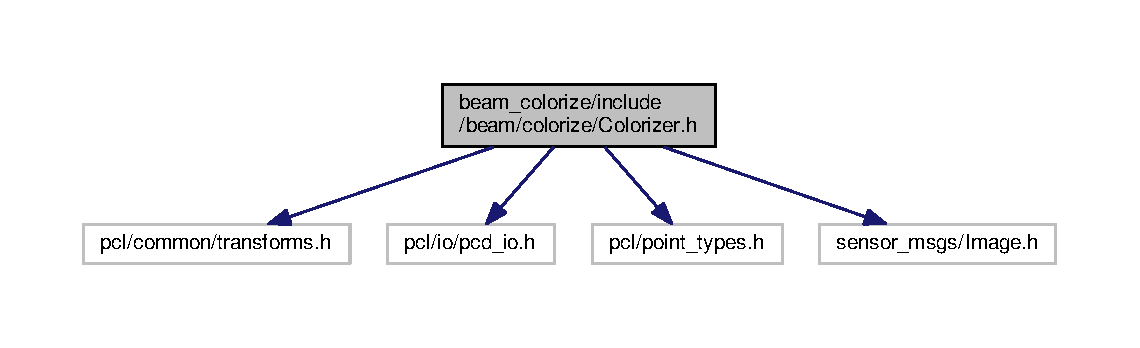
\includegraphics[width=350pt]{_colorizer_8h__incl}
\end{center}
\end{figure}
This graph shows which files directly or indirectly include this file\+:\nopagebreak
\begin{figure}[H]
\begin{center}
\leavevmode
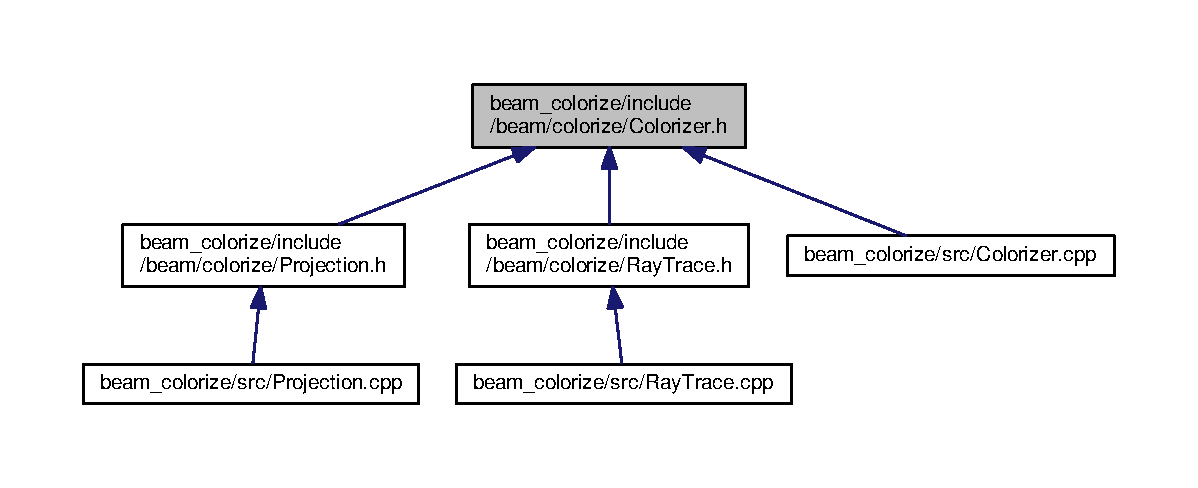
\includegraphics[width=350pt]{_colorizer_8h__dep__incl}
\end{center}
\end{figure}
\subsection*{Classes}
\begin{DoxyCompactItemize}
\item 
class \hyperlink{classbeam__colorize_1_1_colorizer}{beam\+\_\+colorize\+::\+Colorizer}
\begin{DoxyCompactList}\small\item\em Abstract class which different colorization methods can implement. \end{DoxyCompactList}\end{DoxyCompactItemize}
\subsection*{Namespaces}
\begin{DoxyCompactItemize}
\item 
 \hyperlink{namespacebeam__colorize}{beam\+\_\+colorize}
\end{DoxyCompactItemize}


\subsection{Detailed Description}
Includes all colorization classes / functions 
\hypertarget{_projection_8h}{}\section{beam\+\_\+colorize/include/beam/colorize/\+Projection.h File Reference}
\label{_projection_8h}\index{beam\+\_\+colorize/include/beam/colorize/\+Projection.\+h@{beam\+\_\+colorize/include/beam/colorize/\+Projection.\+h}}
{\ttfamily \#include \char`\"{}beam/colorize/\+Colorizer.\+h\char`\"{}}\\*
Include dependency graph for Projection.\+h\+:\nopagebreak
\begin{figure}[H]
\begin{center}
\leavevmode
\includegraphics[width=350pt]{_projection_8h__incl}
\end{center}
\end{figure}
This graph shows which files directly or indirectly include this file\+:\nopagebreak
\begin{figure}[H]
\begin{center}
\leavevmode
\includegraphics[width=241pt]{_projection_8h__dep__incl}
\end{center}
\end{figure}
\subsection*{Classes}
\begin{DoxyCompactItemize}
\item 
class \hyperlink{classbeam__colorize_1_1_projection}{beam\+\_\+colorize\+::\+Projection}
\begin{DoxyCompactList}\small\item\em Class which implements \hyperlink{classbeam__colorize_1_1_colorizer}{Colorizer} interface and provides colorization functionality using projection methods. \end{DoxyCompactList}\end{DoxyCompactItemize}
\subsection*{Namespaces}
\begin{DoxyCompactItemize}
\item 
 \hyperlink{namespacebeam__colorize}{beam\+\_\+colorize}
\end{DoxyCompactItemize}

\hypertarget{_ray_trace_8h}{}\section{beam\+\_\+colorize/include/beam/colorize/\+Ray\+Trace.h File Reference}
\label{_ray_trace_8h}\index{beam\+\_\+colorize/include/beam/colorize/\+Ray\+Trace.\+h@{beam\+\_\+colorize/include/beam/colorize/\+Ray\+Trace.\+h}}
{\ttfamily \#include \char`\"{}beam/colorize/\+Colorizer.\+h\char`\"{}}\\*
Include dependency graph for Ray\+Trace.\+h\+:\nopagebreak
\begin{figure}[H]
\begin{center}
\leavevmode
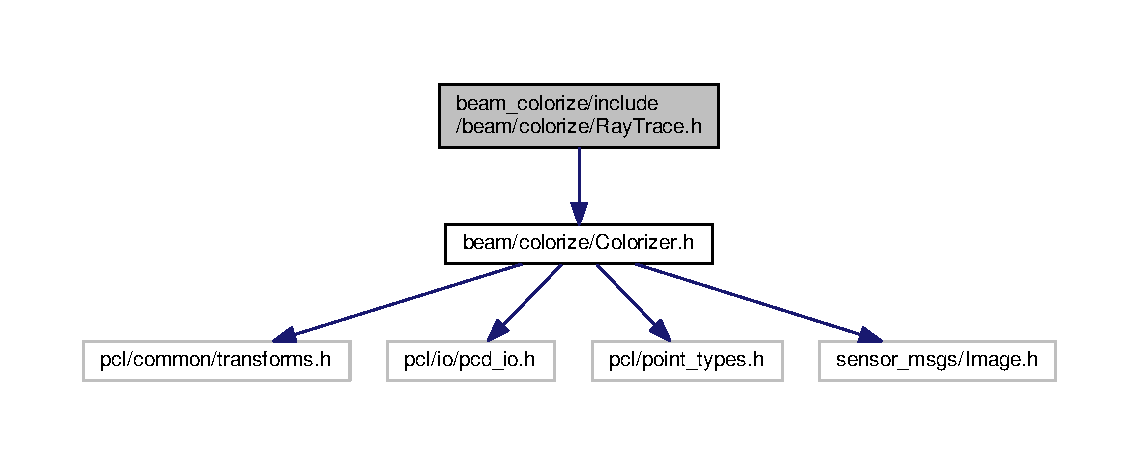
\includegraphics[width=350pt]{_ray_trace_8h__incl}
\end{center}
\end{figure}
This graph shows which files directly or indirectly include this file\+:\nopagebreak
\begin{figure}[H]
\begin{center}
\leavevmode
\includegraphics[width=241pt]{_ray_trace_8h__dep__incl}
\end{center}
\end{figure}
\subsection*{Classes}
\begin{DoxyCompactItemize}
\item 
class \hyperlink{classbeam__colorize_1_1_ray_trace}{beam\+\_\+colorize\+::\+Ray\+Trace}
\begin{DoxyCompactList}\small\item\em Class which implements \hyperlink{classbeam__colorize_1_1_colorizer}{Colorizer} interface and provides colorization functionality using ray tracing. \end{DoxyCompactList}\end{DoxyCompactItemize}
\subsection*{Namespaces}
\begin{DoxyCompactItemize}
\item 
 \hyperlink{namespacebeam__colorize}{beam\+\_\+colorize}
\end{DoxyCompactItemize}

\input{_colorizer_8cpp}
\input{_projection_8cpp}
\input{_ray_trace_8cpp}
\hypertarget{_crack_8h}{}\section{beam\+\_\+defects/include/beam\+\_\+defects/\+Crack.h File Reference}
\label{_crack_8h}\index{beam\+\_\+defects/include/beam\+\_\+defects/\+Crack.\+h@{beam\+\_\+defects/include/beam\+\_\+defects/\+Crack.\+h}}
{\ttfamily \#include \char`\"{}beam\+\_\+defects/\+Defect.\+h\char`\"{}}\\*
Include dependency graph for Crack.\+h\+:\nopagebreak
\begin{figure}[H]
\begin{center}
\leavevmode
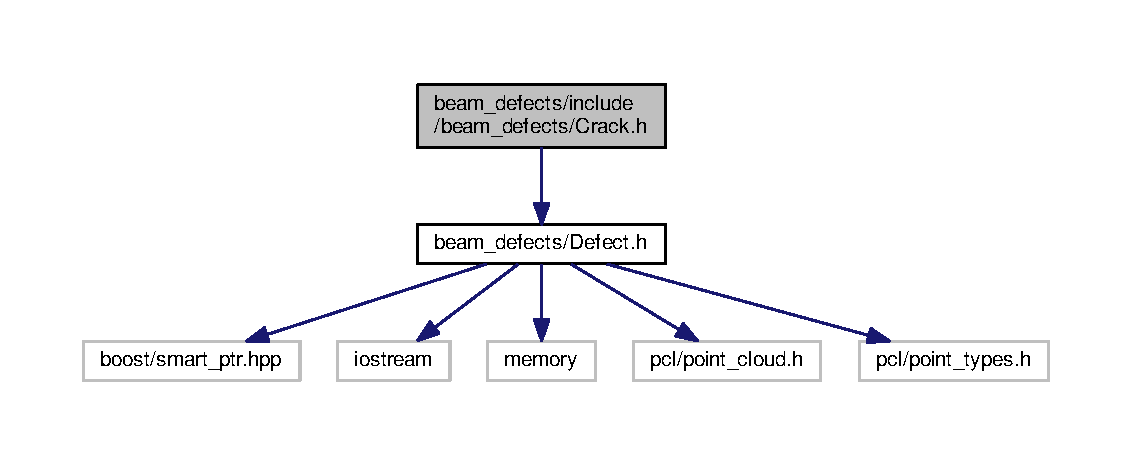
\includegraphics[width=350pt]{_crack_8h__incl}
\end{center}
\end{figure}
This graph shows which files directly or indirectly include this file\+:\nopagebreak
\begin{figure}[H]
\begin{center}
\leavevmode
\includegraphics[width=350pt]{_crack_8h__dep__incl}
\end{center}
\end{figure}
\subsection*{Classes}
\begin{DoxyCompactItemize}
\item 
class \hyperlink{classbeam__defects_1_1_crack}{beam\+\_\+defects\+::\+Crack}
\begin{DoxyCompactList}\small\item\em Derived class for crack defects. \end{DoxyCompactList}\end{DoxyCompactItemize}
\subsection*{Namespaces}
\begin{DoxyCompactItemize}
\item 
 \hyperlink{namespacebeam__defects}{beam\+\_\+defects}
\end{DoxyCompactItemize}

\hypertarget{_defect_8h}{}\section{beam\+\_\+defects/include/beam\+\_\+defects/\+Defect.h File Reference}
\label{_defect_8h}\index{beam\+\_\+defects/include/beam\+\_\+defects/\+Defect.\+h@{beam\+\_\+defects/include/beam\+\_\+defects/\+Defect.\+h}}
{\ttfamily \#include $<$boost/smart\+\_\+ptr.\+hpp$>$}\\*
{\ttfamily \#include $<$iostream$>$}\\*
{\ttfamily \#include $<$memory$>$}\\*
{\ttfamily \#include $<$pcl/point\+\_\+cloud.\+h$>$}\\*
{\ttfamily \#include $<$pcl/point\+\_\+types.\+h$>$}\\*
Include dependency graph for Defect.\+h\+:\nopagebreak
\begin{figure}[H]
\begin{center}
\leavevmode
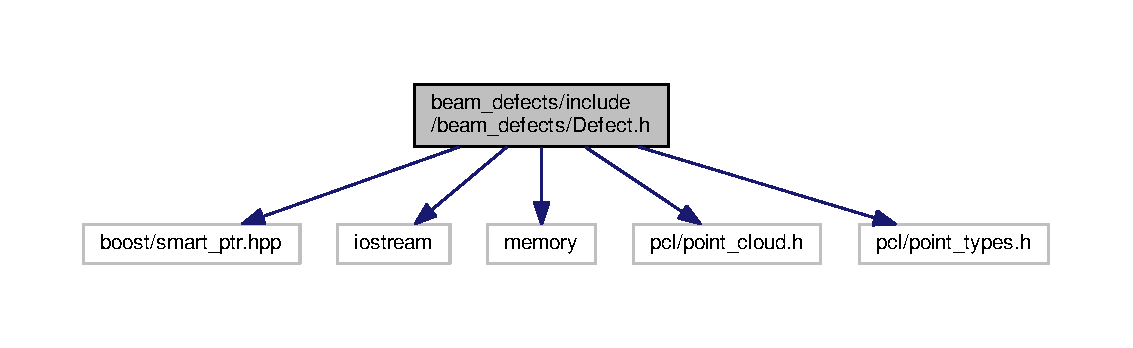
\includegraphics[width=350pt]{_defect_8h__incl}
\end{center}
\end{figure}
This graph shows which files directly or indirectly include this file\+:\nopagebreak
\begin{figure}[H]
\begin{center}
\leavevmode
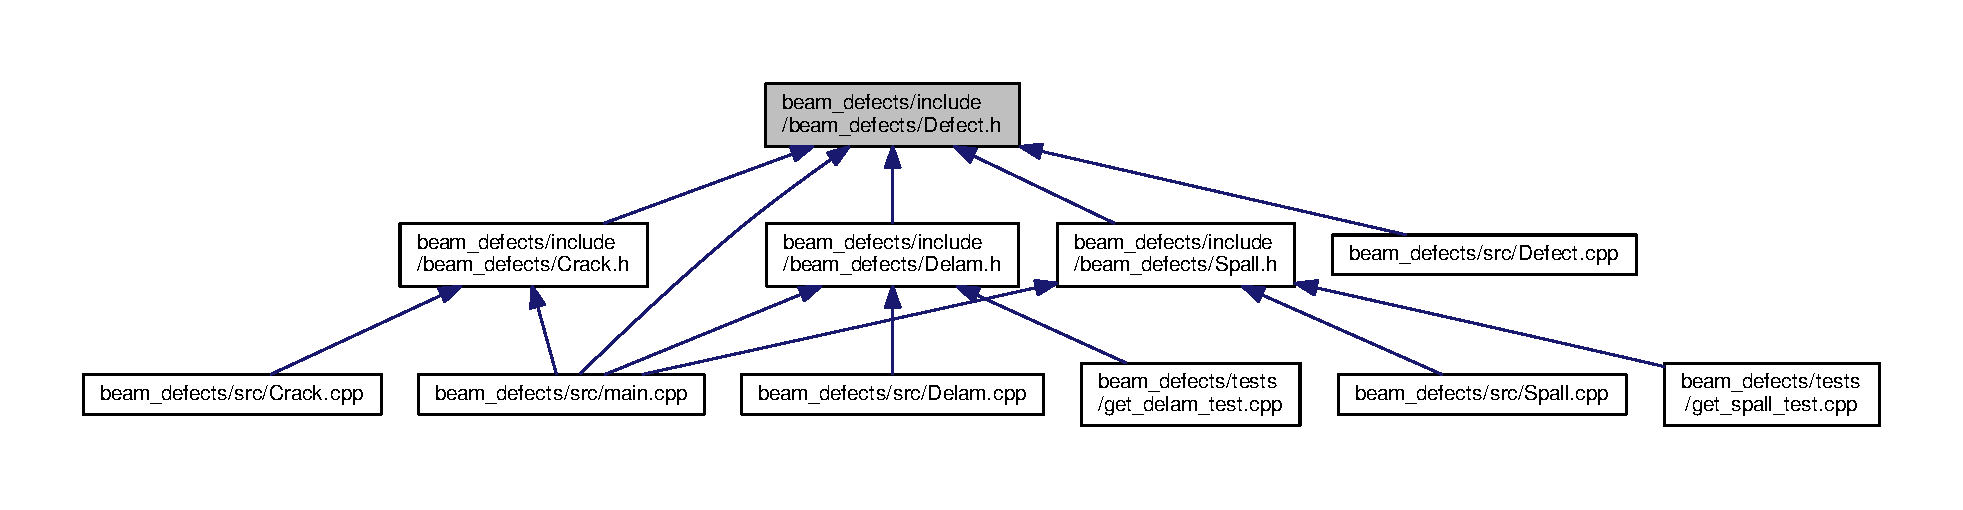
\includegraphics[width=350pt]{_defect_8h__dep__incl}
\end{center}
\end{figure}
\subsection*{Classes}
\begin{DoxyCompactItemize}
\item 
class \hyperlink{classbeam__defects_1_1_defect}{beam\+\_\+defects\+::\+Defect}
\begin{DoxyCompactList}\small\item\em Abstract class for defects. \end{DoxyCompactList}\end{DoxyCompactItemize}
\subsection*{Namespaces}
\begin{DoxyCompactItemize}
\item 
 \hyperlink{namespacebeam__defects}{beam\+\_\+defects}
\end{DoxyCompactItemize}
\subsection*{Enumerations}
\begin{DoxyCompactItemize}
\item 
enum \hyperlink{group__defects_gae379b271bd5fb7ce92afe1abee917249}{beam\+\_\+defects\+::\+Defect\+Type} \{ \hyperlink{group__defects_ggae379b271bd5fb7ce92afe1abee917249a2e6d9801a7e8f255fd21bb5c34d946ae}{beam\+\_\+defects\+::\+Defect\+Type\+::\+C\+R\+A\+CK} = 0, 
\hyperlink{group__defects_ggae379b271bd5fb7ce92afe1abee917249a984e578f1440f286e334efcf3917a453}{beam\+\_\+defects\+::\+Defect\+Type\+::\+S\+P\+A\+LL}, 
\hyperlink{group__defects_ggae379b271bd5fb7ce92afe1abee917249ad2a63853778c868ba1eb01a8be651669}{beam\+\_\+defects\+::\+Defect\+Type\+::\+D\+E\+L\+AM}
 \}\begin{DoxyCompactList}\small\item\em Enum class for different types of defects we might want to use. \end{DoxyCompactList}
\item 
enum \hyperlink{group__defects_gaed38c449f8cba57f35d1af04496a0711}{beam\+\_\+defects\+::\+Defect\+O\+S\+I\+M\+Severity} \{ \\*
\hyperlink{group__defects_ggaed38c449f8cba57f35d1af04496a0711ab50339a10e1de285ac99d4c3990b8693}{beam\+\_\+defects\+::\+Defect\+O\+S\+I\+M\+Severity\+::\+N\+O\+NE} = 0, 
\hyperlink{group__defects_ggaed38c449f8cba57f35d1af04496a0711af8589806bbf66241917092b2a6e18c6f}{beam\+\_\+defects\+::\+Defect\+O\+S\+I\+M\+Severity\+::\+L\+I\+G\+HT}, 
\hyperlink{group__defects_ggaed38c449f8cba57f35d1af04496a0711ac87f3be66ffc3c0d4249f1c2cc5f3cce}{beam\+\_\+defects\+::\+Defect\+O\+S\+I\+M\+Severity\+::\+M\+E\+D\+I\+UM}, 
\hyperlink{group__defects_ggaed38c449f8cba57f35d1af04496a0711a47b0e31408d6208bb828e0b8fa50b3ce}{beam\+\_\+defects\+::\+Defect\+O\+S\+I\+M\+Severity\+::\+S\+E\+V\+E\+RE}, 
\\*
\hyperlink{group__defects_ggaed38c449f8cba57f35d1af04496a0711a6e09e99bef75bdd960bfcf7723422b00}{beam\+\_\+defects\+::\+Defect\+O\+S\+I\+M\+Severity\+::\+V\+E\+R\+Y\+\_\+\+S\+E\+V\+E\+RE}
 \}\begin{DoxyCompactList}\small\item\em Enum class for defect severity based on O\+S\+IM guidelines. \end{DoxyCompactList}
\end{DoxyCompactItemize}


\subsection{Detailed Description}
Includes all defects classes / functions 
\hypertarget{defect__functions_8h}{}\section{beam\+\_\+defects/include/beam\+\_\+defects/defect\+\_\+functions.h File Reference}
\label{defect__functions_8h}\index{beam\+\_\+defects/include/beam\+\_\+defects/defect\+\_\+functions.\+h@{beam\+\_\+defects/include/beam\+\_\+defects/defect\+\_\+functions.\+h}}
{\ttfamily \#include $<$boost/smart\+\_\+ptr.\+hpp$>$}\\*
{\ttfamily \#include $<$pcl/sample\+\_\+consensus/method\+\_\+types.\+h$>$}\\*
{\ttfamily \#include $<$pcl/segmentation/extract\+\_\+clusters.\+h$>$}\\*
{\ttfamily \#include $<$pcl/segmentation/sac\+\_\+segmentation.\+h$>$}\\*
{\ttfamily \#include $<$pcl/surface/concave\+\_\+hull.\+h$>$}\\*
{\ttfamily \#include $<$cmath$>$}\\*
{\ttfamily \#include $<$typeinfo$>$}\\*
{\ttfamily \#include $<$vector$>$}\\*
Include dependency graph for defect\+\_\+functions.\+h\+:\nopagebreak
\begin{figure}[H]
\begin{center}
\leavevmode
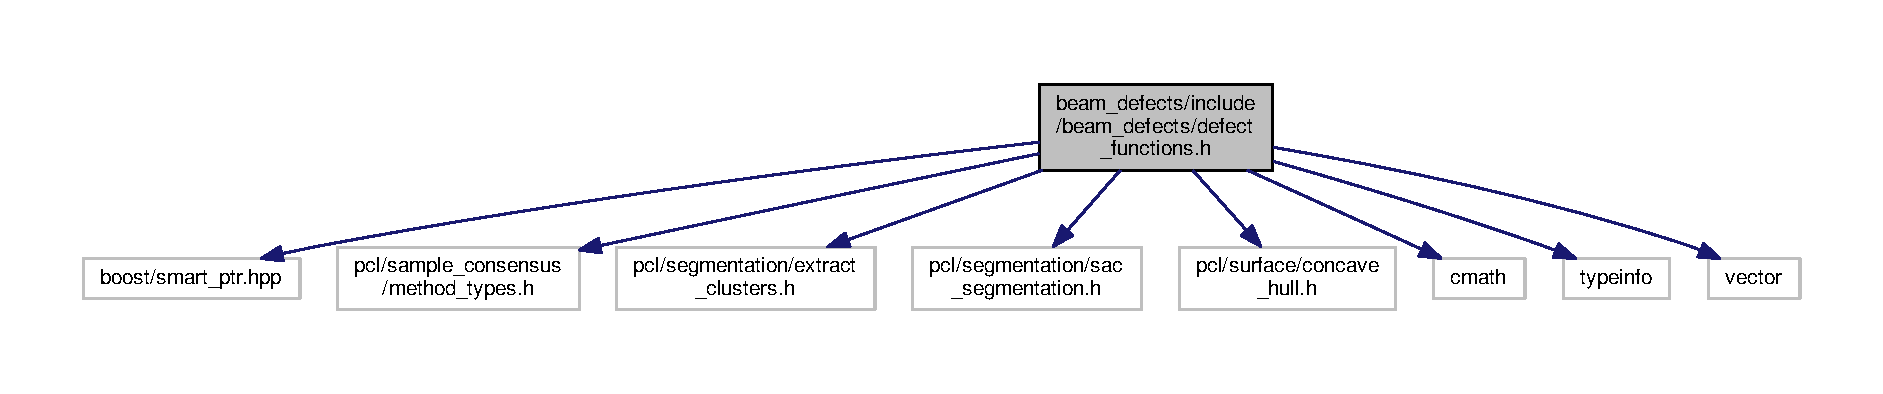
\includegraphics[width=350pt]{defect__functions_8h__incl}
\end{center}
\end{figure}
This graph shows which files directly or indirectly include this file\+:\nopagebreak
\begin{figure}[H]
\begin{center}
\leavevmode
\includegraphics[width=350pt]{defect__functions_8h__dep__incl}
\end{center}
\end{figure}
\subsection*{Namespaces}
\begin{DoxyCompactItemize}
\item 
 \hyperlink{namespacebeam__defects}{beam\+\_\+defects}
\end{DoxyCompactItemize}
\subsection*{Functions}
\begin{DoxyCompactItemize}
\item 
float \hyperlink{group__defects_ga5b7a4f073fbd3207f691f74f63434760}{beam\+\_\+defects\+::dot\+Product} (const std\+::vector$<$ float $>$ \&vect\+\_\+A, const std\+::vector$<$ float $>$ \&vect\+\_\+B)
\item 
std\+::vector$<$ float $>$ \hyperlink{group__defects_gacd54112957db923dfdbe7c0ef41bb462}{beam\+\_\+defects\+::cross\+Product} (const std\+::vector$<$ float $>$ \&vect\+\_\+A, const std\+::vector$<$ float $>$ \&vect\+\_\+B)
\item 
float \hyperlink{group__defects_ga08560ea24958bd0c8ff074c2cb15c946}{beam\+\_\+defects\+::vector\+Length} (const std\+::vector$<$ float $>$ \&vect\+\_\+A)
\item 
std\+::vector$<$ float $>$ \hyperlink{group__defects_ga1f650bbe03aace0d1b8a53291f6f41ed}{beam\+\_\+defects\+::normalize\+Vector} (const std\+::vector$<$ float $>$ \&vect\+\_\+A)
\item 
pcl\+::\+Point\+Cloud$<$ pcl\+::\+Point\+X\+YZ $>$ \hyperlink{group__defects_ga748f611e9ef5f651b856652b0cb5ed7e}{beam\+\_\+defects\+::calculate\+Hull} (const pcl\+::\+Point\+Cloud$<$ pcl\+::\+Point\+X\+YZ $>$\+::Ptr \&input\+\_\+cloud)
\item 
std\+::vector$<$ float $>$ \hyperlink{group__defects_gafee51f4fea21e59f8574542070c232ec}{beam\+\_\+defects\+::plane\+Normal\+Vector} (const pcl\+::\+Point\+Cloud$<$ pcl\+::\+Point\+X\+YZ $>$\+::Ptr \&input\+\_\+cloud)
\item 
pcl\+::\+Point\+Cloud$<$ pcl\+::\+Point\+X\+YZ $>$ \hyperlink{group__defects_ga66ab589a0ee34e37b51df5fed01576c6}{beam\+\_\+defects\+::project2\+Plane} (const pcl\+::\+Point\+Cloud$<$ pcl\+::\+Point\+X\+YZ $>$\+::Ptr \&input\+\_\+cloud, const std\+::vector$<$ float $>$ \&plane\+\_\+norm\+\_\+vect)
\item 
float \hyperlink{group__defects_ga2f624f208e79c917731b7bba9c202a71}{beam\+\_\+defects\+::calculate\+Hull\+Area} (const pcl\+::\+Point\+Cloud$<$ pcl\+::\+Point\+X\+YZ $>$\+::Ptr \&input\+\_\+cloud)
\end{DoxyCompactItemize}

\hypertarget{_delam_8h}{}\section{beam\+\_\+defects/include/beam\+\_\+defects/\+Delam.h File Reference}
\label{_delam_8h}\index{beam\+\_\+defects/include/beam\+\_\+defects/\+Delam.\+h@{beam\+\_\+defects/include/beam\+\_\+defects/\+Delam.\+h}}
{\ttfamily \#include \char`\"{}beam\+\_\+defects/\+Defect.\+h\char`\"{}}\\*
Include dependency graph for Delam.\+h\+:\nopagebreak
\begin{figure}[H]
\begin{center}
\leavevmode
\includegraphics[width=350pt]{_delam_8h__incl}
\end{center}
\end{figure}
This graph shows which files directly or indirectly include this file\+:\nopagebreak
\begin{figure}[H]
\begin{center}
\leavevmode
\includegraphics[width=350pt]{_delam_8h__dep__incl}
\end{center}
\end{figure}
\subsection*{Classes}
\begin{DoxyCompactItemize}
\item 
class \hyperlink{classbeam__defects_1_1_delam}{beam\+\_\+defects\+::\+Delam}
\begin{DoxyCompactList}\small\item\em Derived class for delamination defects. \end{DoxyCompactList}\end{DoxyCompactItemize}
\subsection*{Namespaces}
\begin{DoxyCompactItemize}
\item 
 \hyperlink{namespacebeam__defects}{beam\+\_\+defects}
\end{DoxyCompactItemize}

\hypertarget{_spall_8h}{}\section{beam\+\_\+defects/include/beam\+\_\+defects/\+Spall.h File Reference}
\label{_spall_8h}\index{beam\+\_\+defects/include/beam\+\_\+defects/\+Spall.\+h@{beam\+\_\+defects/include/beam\+\_\+defects/\+Spall.\+h}}
{\ttfamily \#include \char`\"{}beam\+\_\+defects/\+Defect.\+h\char`\"{}}\\*
Include dependency graph for Spall.\+h\+:\nopagebreak
\begin{figure}[H]
\begin{center}
\leavevmode
\includegraphics[width=350pt]{_spall_8h__incl}
\end{center}
\end{figure}
This graph shows which files directly or indirectly include this file\+:\nopagebreak
\begin{figure}[H]
\begin{center}
\leavevmode
\includegraphics[width=350pt]{_spall_8h__dep__incl}
\end{center}
\end{figure}
\subsection*{Classes}
\begin{DoxyCompactItemize}
\item 
class \hyperlink{classbeam__defects_1_1_spall}{beam\+\_\+defects\+::\+Spall}
\begin{DoxyCompactList}\small\item\em Derived class for spall defects. \end{DoxyCompactList}\end{DoxyCompactItemize}
\subsection*{Namespaces}
\begin{DoxyCompactItemize}
\item 
 \hyperlink{namespacebeam__defects}{beam\+\_\+defects}
\end{DoxyCompactItemize}

\input{_crack_8cpp}
\input{_defect_8cpp}
\input{defect__functions_8cpp}
\input{_delam_8cpp}
\input{main_8cpp}
\input{_spall_8cpp}
\input{get__delam__test_8cpp}
\input{get__spall__test_8cpp}
\input{angles_8hpp}
\hypertarget{config_8hpp}{}\section{beam\+\_\+utils/include/beam/utils/config.hpp File Reference}
\label{config_8hpp}\index{beam\+\_\+utils/include/beam/utils/config.\+hpp@{beam\+\_\+utils/include/beam/utils/config.\+hpp}}
{\ttfamily \#include $<$iostream$>$}\\*
{\ttfamily \#include $<$sstream$>$}\\*
{\ttfamily \#include $<$string$>$}\\*
{\ttfamily \#include $<$type\+\_\+traits$>$}\\*
{\ttfamily \#include $<$yaml-\/cpp/yaml.\+h$>$}\\*
{\ttfamily \#include \char`\"{}beam/utils/log.\+hpp\char`\"{}}\\*
{\ttfamily \#include \char`\"{}beam/utils/math.\+hpp\char`\"{}}\\*
Include dependency graph for config.\+hpp\+:\nopagebreak
\begin{figure}[H]
\begin{center}
\leavevmode
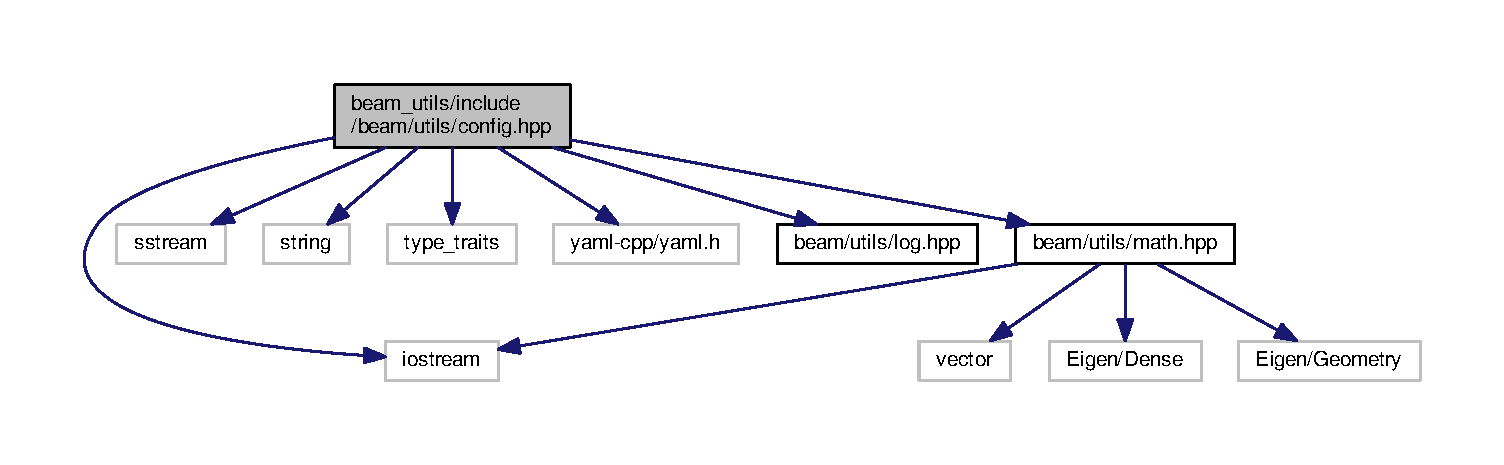
\includegraphics[width=350pt]{config_8hpp__incl}
\end{center}
\end{figure}
This graph shows which files directly or indirectly include this file\+:\nopagebreak
\begin{figure}[H]
\begin{center}
\leavevmode
\includegraphics[width=330pt]{config_8hpp__dep__incl}
\end{center}
\end{figure}
\subsection*{Classes}
\begin{DoxyCompactItemize}
\item 
struct \hyperlink{structbeam_1_1_config_param_base}{beam\+::\+Config\+Param\+Base}
\item 
class \hyperlink{classbeam_1_1_config_param}{beam\+::\+Config\+Param$<$ T $>$}
\item 
class \hyperlink{classbeam_1_1_config_parser}{beam\+::\+Config\+Parser}
\item 
struct \hyperlink{struct_y_a_m_l_1_1convert_3_01_eigen_1_1_matrix_3_01_scalar_00_01_rows_00_01_cols_01_4_01_4}{Y\+A\+M\+L\+::convert$<$ Eigen\+::\+Matrix$<$ Scalar, Rows, Cols $>$ $>$}
\item 
struct \hyperlink{struct_y_a_m_l_1_1convert_3_01_eigen_1_1_matrix_3_01_scalar_00_01_rows_00_011_01_4_01_4}{Y\+A\+M\+L\+::convert$<$ Eigen\+::\+Matrix$<$ Scalar, Rows, 1 $>$ $>$}
\end{DoxyCompactItemize}
\subsection*{Namespaces}
\begin{DoxyCompactItemize}
\item 
 \hyperlink{namespacebeam}{beam}
\item 
 \hyperlink{namespace_y_a_m_l}{Y\+A\+ML}
\end{DoxyCompactItemize}
\subsection*{Enumerations}
\begin{DoxyCompactItemize}
\item 
enum \hyperlink{group__utils_ga6b948c6f49abd3a3de95390efacfba63}{beam\+::\+Config\+Status} \{ \\*
\hyperlink{group__utils_gga6b948c6f49abd3a3de95390efacfba63ae0aa021e21dddbd6d8cecec71e9cf564}{beam\+::\+Config\+Status\+::\+OK} = 0, 
\hyperlink{group__utils_gga6b948c6f49abd3a3de95390efacfba63ab150e1b84c6f67e2bebfa5a682f71a37}{beam\+::\+Config\+Status\+::\+Missing\+Optional\+Key} = 1, 
\hyperlink{group__utils_gga6b948c6f49abd3a3de95390efacfba63a06344c468073b2b66824779ffa5105cc}{beam\+::\+Config\+Status\+::\+File\+Error} = -\/1, 
\hyperlink{group__utils_gga6b948c6f49abd3a3de95390efacfba63ac84999914a408f8c02b4122a49df6e00}{beam\+::\+Config\+Status\+::\+Key\+Error} = -\/2, 
\\*
\hyperlink{group__utils_gga6b948c6f49abd3a3de95390efacfba63a33f8a28d3c790e00d94cc848895dfb51}{beam\+::\+Config\+Status\+::\+Conversion\+Error} = -\/3
 \}
\end{DoxyCompactItemize}


\subsection{Detailed Description}
Contains a useful {\ttfamily Config\+Parser} class to simplify parsing yaml files. 
\hypertarget{log_8hpp}{}\section{beam\+\_\+utils/include/beam/utils/log.hpp File Reference}
\label{log_8hpp}\index{beam\+\_\+utils/include/beam/utils/log.\+hpp@{beam\+\_\+utils/include/beam/utils/log.\+hpp}}
This graph shows which files directly or indirectly include this file\+:\nopagebreak
\begin{figure}[H]
\begin{center}
\leavevmode
\includegraphics[width=350pt]{log_8hpp__dep__incl}
\end{center}
\end{figure}
\subsection*{Namespaces}
\begin{DoxyCompactItemize}
\item 
 \hyperlink{namespacebeam}{beam}
\end{DoxyCompactItemize}
\subsection*{Macros}
\begin{DoxyCompactItemize}
\item 
\#define \hyperlink{group__utils_ga8de29f7c8bbf1a81cc6e71ac602032d3}{F\+I\+L\+E\+N\+A\+ME}~(strrchr(\+\_\+\+\_\+\+F\+I\+L\+E\+\_\+\+\_\+, \textquotesingle{}/\textquotesingle{}) ? strrchr(\+\_\+\+\_\+\+F\+I\+L\+E\+\_\+\+\_\+, \textquotesingle{}/\textquotesingle{}) + 1 \+: \+\_\+\+\_\+\+F\+I\+L\+E\+\_\+\+\_\+)
\item 
\#define \hyperlink{group__utils_ga187d17bb2372f3cc639923dba56dad1b}{L\+O\+G\+\_\+\+E\+R\+R\+OR}(M, ...)
\item 
\#define \hyperlink{group__utils_ga2ea0e9153d7e590b2b2b6c2bee498a76}{L\+O\+G\+\_\+\+I\+N\+FO}(M, ...)~fprintf(stdout, \char`\"{}\mbox{[}I\+N\+FO\mbox{]} \char`\"{} M \char`\"{}\textbackslash{}n\char`\"{}, \#\#\+\_\+\+\_\+\+V\+A\+\_\+\+A\+R\+G\+S\+\_\+\+\_\+)
\end{DoxyCompactItemize}


\subsection{Detailed Description}
Functions to log errors and info to {\ttfamily stderr} and {\ttfamily stdout}.

{\ttfamily L\+O\+G\+\_\+\+E\+R\+R\+OR} and {\ttfamily L\+O\+G\+\_\+\+I\+N\+FO} both are simple {\ttfamily fprintf()} that can be use to write message {\ttfamily M} to {\ttfamily stderr} and {\ttfamily stdout}. For example\+: 
\begin{DoxyCode}
\hyperlink{group__utils_ga187d17bb2372f3cc639923dba56dad1b}{LOG\_ERROR}(\textcolor{stringliteral}{"Failed to load configuration file [%s]"}, config\_file.c\_str());
\hyperlink{group__utils_ga2ea0e9153d7e590b2b2b6c2bee498a76}{LOG\_INFO}(\textcolor{stringliteral}{"Parameter was not found! Loading defaults!"});
\end{DoxyCode}
 
\hypertarget{math_8hpp}{}\section{beam\+\_\+utils/include/beam/utils/math.hpp File Reference}
\label{math_8hpp}\index{beam\+\_\+utils/include/beam/utils/math.\+hpp@{beam\+\_\+utils/include/beam/utils/math.\+hpp}}
{\ttfamily \#include $<$iostream$>$}\\*
{\ttfamily \#include $<$vector$>$}\\*
{\ttfamily \#include $<$Eigen/\+Dense$>$}\\*
{\ttfamily \#include $<$Eigen/\+Geometry$>$}\\*
Include dependency graph for math.\+hpp\+:\nopagebreak
\begin{figure}[H]
\begin{center}
\leavevmode
\includegraphics[width=350pt]{math_8hpp__incl}
\end{center}
\end{figure}
This graph shows which files directly or indirectly include this file\+:\nopagebreak
\begin{figure}[H]
\begin{center}
\leavevmode
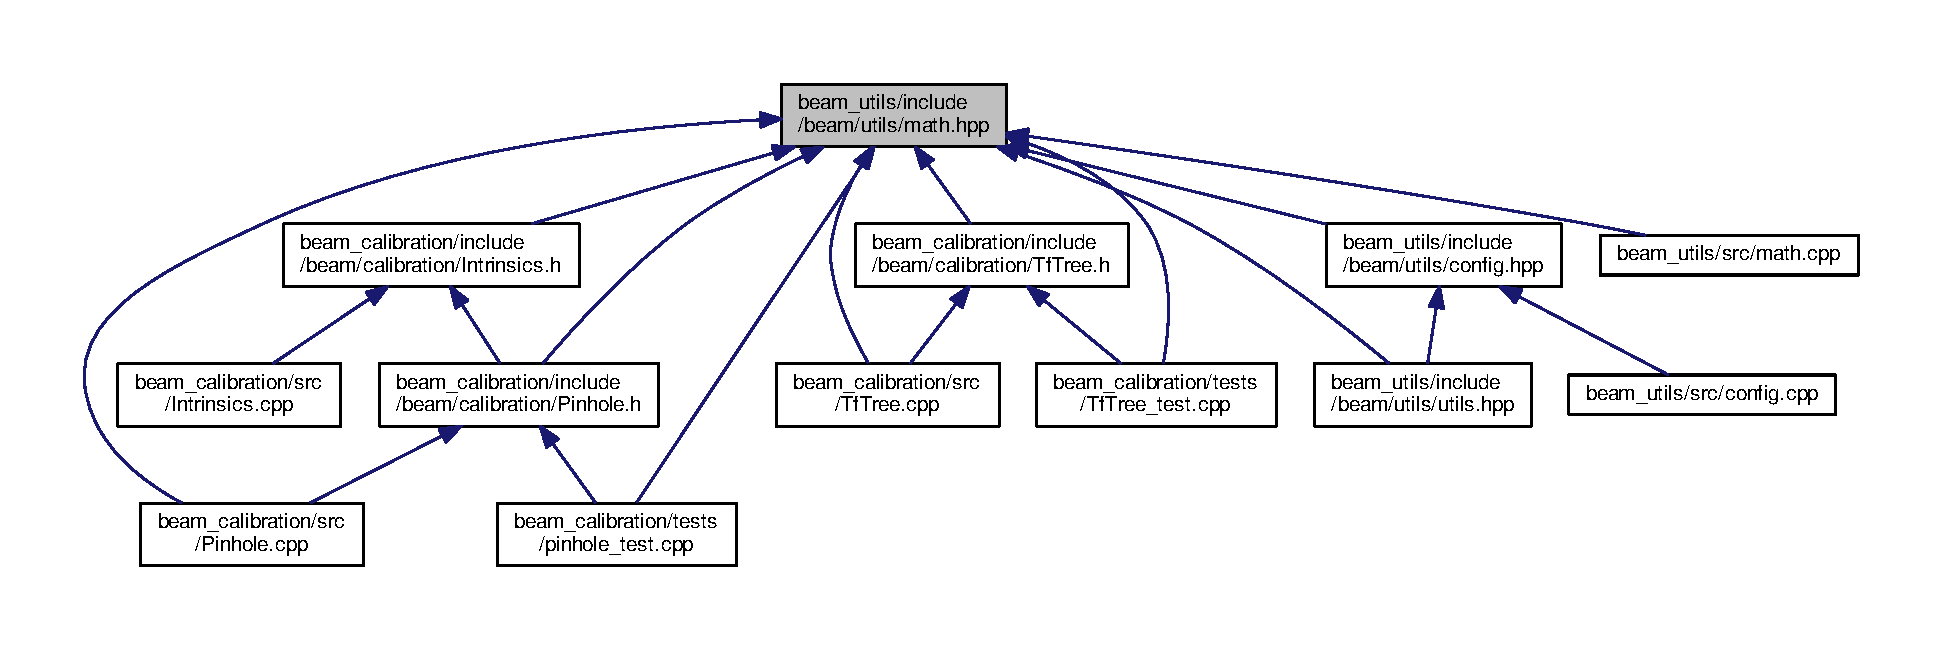
\includegraphics[width=350pt]{math_8hpp__dep__incl}
\end{center}
\end{figure}
\subsection*{Classes}
\begin{DoxyCompactItemize}
\item 
struct \hyperlink{structbeam_1_1_vec_comparator}{beam\+::\+Vec\+Comparator}
\item 
struct \hyperlink{structbeam_1_1_mat_comparator}{beam\+::\+Mat\+Comparator}
\end{DoxyCompactItemize}
\subsection*{Namespaces}
\begin{DoxyCompactItemize}
\item 
 \hyperlink{namespacebeam}{beam}
\end{DoxyCompactItemize}
\subsection*{Macros}
\begin{DoxyCompactItemize}
\item 
\#define \hyperlink{group__utils_ga9f2375aee996fb13eecdf9eab8aceb6e}{B\+E\+A\+M\+\_\+\+E\+I\+G\+E\+N\+\_\+\+T\+Y\+P\+E\+D\+EF}
\end{DoxyCompactItemize}
\subsection*{Typedefs}
\begin{DoxyCompactItemize}
\item 
typedef Eigen\+::\+Vector2d \hyperlink{group__utils_ga6112bda54e53755ab14060144285c6b0}{beam\+::\+Vec2}
\item 
typedef Eigen\+::\+Vector3d \hyperlink{group__utils_ga7aca82b90a74cb643417801e830cd43f}{beam\+::\+Vec3}
\item 
typedef Eigen\+::\+Vector4d \hyperlink{group__utils_gae8c630e8f7e9cdbc1a7dcc3073a99d5c}{beam\+::\+Vec4}
\item 
typedef Eigen\+::\+Matrix$<$ double, 5, 1 $>$ \hyperlink{group__utils_gabd17e53e0e9320ff4dcbad3b0e591928}{beam\+::\+Vec5}
\item 
typedef Eigen\+::\+Matrix$<$ double, 6, 1 $>$ \hyperlink{group__utils_ga9f18e27181a175dfd15dc192a7d417d1}{beam\+::\+Vec6}
\item 
typedef Eigen\+::\+Vector\+Xd \hyperlink{group__utils_gae5ba967e4b0d4b421ca30ef46f896145}{beam\+::\+VecX}
\item 
typedef Eigen\+::\+Matrix2d \hyperlink{group__utils_gaa647b85b058c8a50386a3da8dd719e3d}{beam\+::\+Mat2}
\item 
typedef Eigen\+::\+Matrix3d \hyperlink{group__utils_ga665fed2673de952d12b19351a2bdb961}{beam\+::\+Mat3}
\item 
typedef Eigen\+::\+Matrix4d \hyperlink{group__utils_ga06979ede648a91a7e5465980784ebb1b}{beam\+::\+Mat4}
\item 
typedef Eigen\+::\+Matrix$<$ double, 5, 5 $>$ \hyperlink{group__utils_ga34f1d113f166129c5b89fe92c5a07e02}{beam\+::\+Mat5}
\item 
typedef Eigen\+::\+Matrix$<$ double, 6, 6 $>$ \hyperlink{group__utils_gac42e2f9ad085d2fcc34875015c43cecc}{beam\+::\+Mat6}
\item 
typedef Eigen\+::\+Matrix\+Xd \hyperlink{group__utils_gaf1ee9917aef6e6cf513d29f8c7d2eeee}{beam\+::\+MatX}
\item 
typedef Eigen\+::\+Affine3d \hyperlink{group__utils_ga609e7e934806a61b3cb511b893f799ce}{beam\+::\+Affine3}
\item 
typedef Eigen\+::\+Quaterniond \hyperlink{group__utils_gab34e0dc5bdfa343eebf793fdc084a07f}{beam\+::\+Quaternion}
\end{DoxyCompactItemize}
\subsection*{Functions}
\begin{DoxyCompactItemize}
\item 
int \hyperlink{group__utils_ga1709c3968d710a88b5cc6b034358ff4b}{beam\+::randi} (int ub, int lb)
\item 
double \hyperlink{group__utils_gaf3391ec0a035372eb7fa27646aa97018}{beam\+::randf} (double ub, double lb)
\item 
int \hyperlink{group__utils_gacf5e889cd118230c90c1618324b47644}{beam\+::fltcmp} (double f1, double f2, double threshold=0.\+0001)
\item 
double \hyperlink{group__utils_ga78b63ada78026ee09e93e996a6da095b}{beam\+::median} (std\+::vector$<$ double $>$ v)
\item 
void \hyperlink{group__utils_ga1c462df8889ae3641889e12d7491e995}{beam\+::vec2mat} (std\+::vector$<$ double $>$ x, int rows, int cols, MatX \&y)
\item 
void \hyperlink{group__utils_gac7f5f2ea3f1feec3cedfc2b0f61aff90}{beam\+::mat2vec} (MatX A, std\+::vector$<$ double $>$ \&x)
\item 
int \hyperlink{group__utils_ga986bd09d39d65902c831209a1f311819}{beam\+::euler2rot} (Vec3 euler, int euler\+\_\+seq, Mat3 \&R)
\item 
int \hyperlink{group__utils_ga87a6d391d78520ba96a429f65d06bb84}{beam\+::euler2quat} (Vec3 euler, int euler\+\_\+seq, Quaternion \&q)
\item 
int \hyperlink{group__utils_ga15d4558557dc0197de74a7ae56daa53f}{beam\+::quat2euler} (Quaternion q, int euler\+\_\+seq, Vec3 \&euler)
\item 
int \hyperlink{group__utils_ga99cfa04b1c384ead4ae82b4cc4843a5c}{beam\+::quat2rot} (Quaternion q, Mat3 \&R)
\item 
void \hyperlink{group__utils_ga5fe56de851463d297a144a0eb5e7e1b2}{beam\+::enu2nwu} (const Vec3 \&enu, Vec3 \&nwu)
\item 
void \hyperlink{group__utils_ga6e0ef288576925f8c79fd3284743e86c}{beam\+::ned2enu} (const Vec3 \&ned, Vec3 \&enu)
\item 
void \hyperlink{group__utils_ga82aa198fb08b86d9b4fb0854e09acdca}{beam\+::ned2nwu} (const Quaternion \&ned, Quaternion \&enu)
\item 
void \hyperlink{group__utils_gaec5283955c5b5122e00b7fb38b1d69c5}{beam\+::nwu2enu} (const Vec3 \&nwu, Vec3 \&enu)
\item 
void \hyperlink{group__utils_ga7f2d193025c27530e4736c9fabba6aeb}{beam\+::nwu2ned} (const Quaternion \&nwu, Quaternion \&ned)
\item 
void \hyperlink{group__utils_gacd46e4e0d954431486c743882f04b1a3}{beam\+::nwu2edn} (const Vec3 \&nwu, Vec3 \&edn)
\end{DoxyCompactItemize}


\subsection{Detailed Description}
Utility mathematical functions that do not fit anywhere else.

The type definitions are shorthands for declaring {\ttfamily Eigen\+::\+Vector}, {\ttfamily Eigen\+::\+Matrix} and {\ttfamily Eigen\+::\+Quaternion} objects. At current we assume all slam code development will be using double precision floating points. 
\hypertarget{time_8hpp}{}\section{beam\+\_\+utils/include/beam/utils/time.hpp File Reference}
\label{time_8hpp}\index{beam\+\_\+utils/include/beam/utils/time.\+hpp@{beam\+\_\+utils/include/beam/utils/time.\+hpp}}
{\ttfamily \#include $<$time.\+h$>$}\\*
{\ttfamily \#include $<$sys/time.\+h$>$}\\*
Include dependency graph for time.\+hpp\+:\nopagebreak
\begin{figure}[H]
\begin{center}
\leavevmode
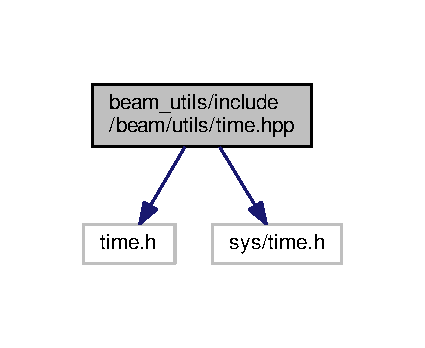
\includegraphics[width=204pt]{time_8hpp__incl}
\end{center}
\end{figure}
This graph shows which files directly or indirectly include this file\+:\nopagebreak
\begin{figure}[H]
\begin{center}
\leavevmode
\includegraphics[width=324pt]{time_8hpp__dep__incl}
\end{center}
\end{figure}
\subsection*{Namespaces}
\begin{DoxyCompactItemize}
\item 
 \hyperlink{namespacebeam}{beam}
\end{DoxyCompactItemize}
\subsection*{Functions}
\begin{DoxyCompactItemize}
\item 
void \hyperlink{group__utils_gaaebadeacafd2b1816dab04b0db7147f6}{beam\+::tic} (struct timespec $\ast$tic)
\item 
float \hyperlink{group__utils_gabe4bc58525b5b33ead190307009c9335}{beam\+::toc} (struct timespec $\ast$tic)
\item 
float \hyperlink{group__utils_gab928984bd87de1db648f2b349fdeac74}{beam\+::mtoc} (struct timespec $\ast$tic)
\item 
double \hyperlink{group__utils_gab7f144a34f327358efbe5c08af63fdb7}{beam\+::time\+\_\+now} (void)
\end{DoxyCompactItemize}


\subsection{Detailed Description}
Timing functions, useful for measuring how long a particular function executed, etc. 
\hypertarget{utils_8hpp}{}\section{beam\+\_\+utils/include/beam/utils/utils.hpp File Reference}
\label{utils_8hpp}\index{beam\+\_\+utils/include/beam/utils/utils.\+hpp@{beam\+\_\+utils/include/beam/utils/utils.\+hpp}}
{\ttfamily \#include \char`\"{}beam/utils/config.\+hpp\char`\"{}}\\*
{\ttfamily \#include \char`\"{}beam/utils/math.\+hpp\char`\"{}}\\*
{\ttfamily \#include \char`\"{}beam/utils/time.\+hpp\char`\"{}}\\*
{\ttfamily \#include \char`\"{}beam/utils/angles.\+hpp\char`\"{}}\\*
Include dependency graph for utils.\+hpp\+:\nopagebreak
\begin{figure}[H]
\begin{center}
\leavevmode
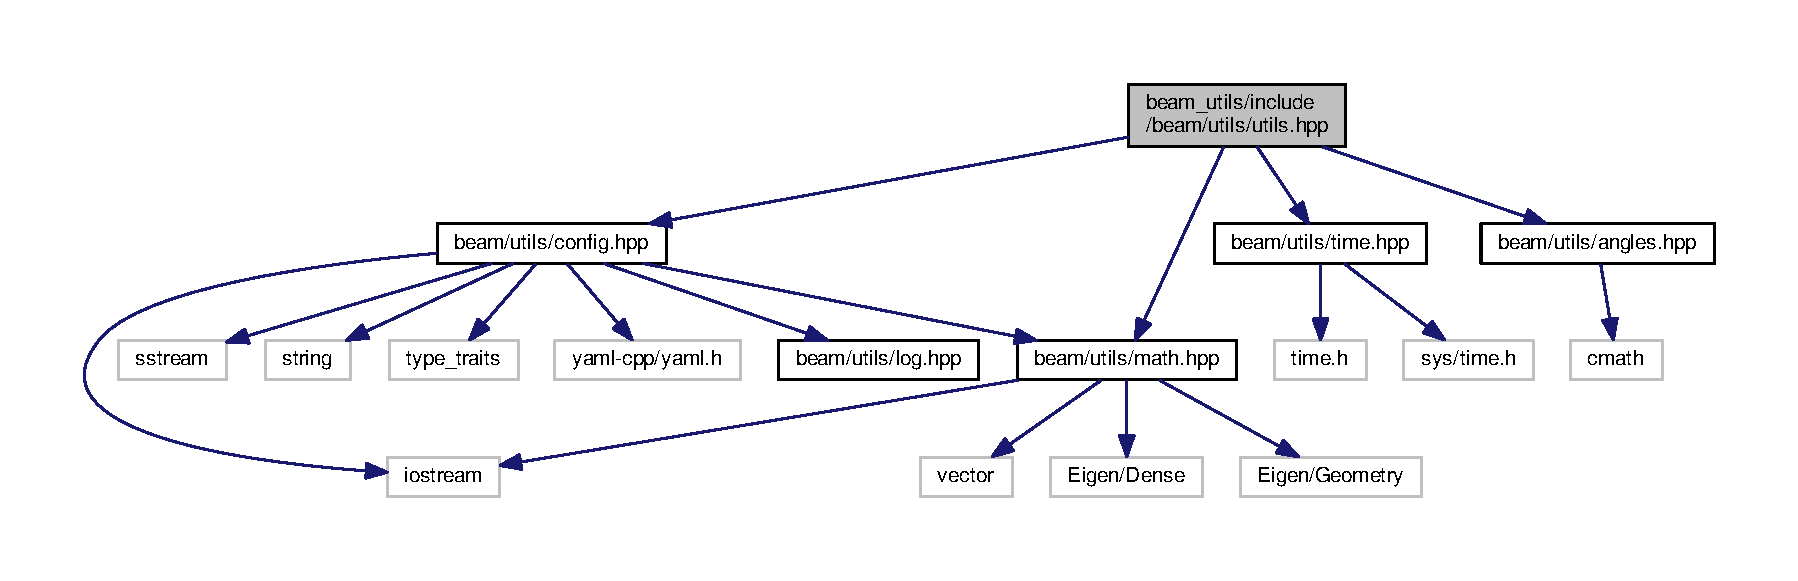
\includegraphics[width=350pt]{utils_8hpp__incl}
\end{center}
\end{figure}


\subsection{Detailed Description}
Includes all utility functions 
\input{angles_8cpp}
\input{config_8cpp}
\input{math_8cpp}
\input{time_8cpp}
\input{build_2catkin__generated_2generate__cached__setup_8py}
\input{cmake-build-debug_2catkin__generated_2generate__cached__setup_8py}
\input{cmake-build-release-gcc83_2catkin__generated_2generate__cached__setup_8py}
\input{build_2catkin__generated_2installspace_2__setup__util_8py}
\input{build_2devel_2__setup__util_8py}
\input{cmake-build-debug_2beam__calibration_2catkin__generated_2installspace_2__setup__util_8py}
\input{cmake-build-debug_2beam__colorize_2catkin__generated_2installspace_2__setup__util_8py}
\input{cmake-build-debug_2catkin__generated_2installspace_2__setup__util_8py}
\input{cmake-build-debug_2devel_2__setup__util_8py}
\input{cmake-build-release-gcc83_2beam__calibration_2catkin__generated_2installspace_2__setup__util_8py}
\input{cmake-build-release-gcc83_2beam__colorize_2catkin__generated_2installspace_2__setup__util_8py}
\input{cmake-build-release-gcc83_2catkin__generated_2installspace_2__setup__util_8py}
\input{cmake-build-release-gcc83_2devel_2__setup__util_8py}
\input{build_2_c_make_files_23_814_820190327-gd2c03_2_compiler_id_c_2_c_make_c_compiler_id_8c}
\input{cmake-build-debug_2_c_make_files_23_813_84_2_compiler_id_c_2_c_make_c_compiler_id_8c}
\input{cmake-build-release-gcc83_2_c_make_files_23_814_820190327-gd2c03_2_compiler_id_c_2_c_make_c_compiler_id_8c}
\input{build_2_c_make_files_23_814_820190327-gd2c03_2_compiler_id_c_x_x_2_c_make_c_x_x_compiler_id_8cpp}
\input{cmake-build-debug_2_c_make_files_23_813_84_2_compiler_id_c_x_x_2_c_make_c_x_x_compiler_id_8cpp}
\input{cmake-build-release-gcc83_2_c_make_files_23_814_820190327-gd2c03_2_compiler_id_c_x_x_2_c_make_c_x_x_compiler_id_8cpp}
\input{build_2_c_make_files_2feature__tests_8c}
\input{cmake-build-debug_2_c_make_files_2feature__tests_8c}
\input{cmake-build-release-gcc83_2_c_make_files_2feature__tests_8c}
\input{build_2_c_make_files_2feature__tests_8cxx}
\input{cmake-build-debug_2_c_make_files_2feature__tests_8cxx}
\input{cmake-build-release-gcc83_2_c_make_files_2feature__tests_8cxx}
\input{_r_e_a_d_m_e_8md}
%--- End generated contents ---

% Index
\backmatter
\newpage
\phantomsection
\clearemptydoublepage
\addcontentsline{toc}{chapter}{Index}
\printindex

\end{document}
